\documentclass[twoside]{book}

% Packages required by doxygen
\usepackage{fixltx2e}
\usepackage{calc}
\usepackage{doxygen}
\usepackage[export]{adjustbox} % also loads graphicx
\usepackage{graphicx}
\usepackage[utf8]{inputenc}
\usepackage{makeidx}
\usepackage{multicol}
\usepackage{multirow}
\PassOptionsToPackage{warn}{textcomp}
\usepackage{textcomp}
\usepackage[nointegrals]{wasysym}
\usepackage[table]{xcolor}

% Font selection
\usepackage[T1]{fontenc}
\usepackage[scaled=.90]{helvet}
\usepackage{courier}
\usepackage{amssymb}
\usepackage{sectsty}
\renewcommand{\familydefault}{\sfdefault}
\allsectionsfont{%
  \fontseries{bc}\selectfont%
  \color{darkgray}%
}
\renewcommand{\DoxyLabelFont}{%
  \fontseries{bc}\selectfont%
  \color{darkgray}%
}
\newcommand{\+}{\discretionary{\mbox{\scriptsize$\hookleftarrow$}}{}{}}

% Page & text layout
\usepackage{geometry}
\geometry{%
  a4paper,%
  top=2.5cm,%
  bottom=2.5cm,%
  left=2.5cm,%
  right=2.5cm%
}
\tolerance=750
\hfuzz=15pt
\hbadness=750
\setlength{\emergencystretch}{15pt}
\setlength{\parindent}{0cm}
\setlength{\parskip}{3ex plus 2ex minus 2ex}
\makeatletter
\renewcommand{\paragraph}{%
  \@startsection{paragraph}{4}{0ex}{-1.0ex}{1.0ex}{%
    \normalfont\normalsize\bfseries\SS@parafont%
  }%
}
\renewcommand{\subparagraph}{%
  \@startsection{subparagraph}{5}{0ex}{-1.0ex}{1.0ex}{%
    \normalfont\normalsize\bfseries\SS@subparafont%
  }%
}
\makeatother

% Headers & footers
\usepackage{fancyhdr}
\pagestyle{fancyplain}
\fancyhead[LE]{\fancyplain{}{\bfseries\thepage}}
\fancyhead[CE]{\fancyplain{}{}}
\fancyhead[RE]{\fancyplain{}{\bfseries\leftmark}}
\fancyhead[LO]{\fancyplain{}{\bfseries\rightmark}}
\fancyhead[CO]{\fancyplain{}{}}
\fancyhead[RO]{\fancyplain{}{\bfseries\thepage}}
\fancyfoot[LE]{\fancyplain{}{}}
\fancyfoot[CE]{\fancyplain{}{}}
\fancyfoot[RE]{\fancyplain{}{\bfseries\scriptsize Generated by Doxygen }}
\fancyfoot[LO]{\fancyplain{}{\bfseries\scriptsize Generated by Doxygen }}
\fancyfoot[CO]{\fancyplain{}{}}
\fancyfoot[RO]{\fancyplain{}{}}
\renewcommand{\footrulewidth}{0.4pt}
\renewcommand{\chaptermark}[1]{%
  \markboth{#1}{}%
}
\renewcommand{\sectionmark}[1]{%
  \markright{\thesection\ #1}%
}

% Indices & bibliography
\usepackage{natbib}
\usepackage[titles]{tocloft}
\setcounter{tocdepth}{3}
\setcounter{secnumdepth}{5}
\makeindex

% Hyperlinks (required, but should be loaded last)
\usepackage{ifpdf}
\ifpdf
  \usepackage[pdftex,pagebackref=true]{hyperref}
\else
  \usepackage[ps2pdf,pagebackref=true]{hyperref}
\fi
\hypersetup{%
  colorlinks=true,%
  linkcolor=blue,%
  citecolor=blue,%
  unicode%
}

% Custom commands
\newcommand{\clearemptydoublepage}{%
  \newpage{\pagestyle{empty}\cleardoublepage}%
}

\usepackage{caption}
\captionsetup{labelsep=space,justification=centering,font={bf},singlelinecheck=off,skip=4pt,position=top}

%===== C O N T E N T S =====

\begin{document}

% Titlepage & ToC
\hypersetup{pageanchor=false,
             bookmarksnumbered=true,
             pdfencoding=unicode
            }
\pagenumbering{alph}
\begin{titlepage}
\vspace*{7cm}
\begin{center}%
{\Large C\+U\+DA Urb \\[1ex]\large 1.\+0 }\\
\vspace*{1cm}
{\large Generated by Doxygen 1.8.13}\\
\end{center}
\end{titlepage}
\clearemptydoublepage
\pagenumbering{roman}
\tableofcontents
\clearemptydoublepage
\pagenumbering{arabic}
\hypersetup{pageanchor=true}

%--- Begin generated contents ---
\chapter{C\+U\+D\+A-\/\+U\+RB code}
\label{index}\hypertarget{index}{}\begin{DoxyAuthor}{Author}
Behnam Bozorgmehr 
\end{DoxyAuthor}
\begin{DoxyVersion}{Version}
1.\+0 
\end{DoxyVersion}
\begin{DoxyDate}{Date}
06/04/2018 
\end{DoxyDate}
\begin{DoxyCopyright}{Copyright}
G\+NU Public License
\end{DoxyCopyright}
\hypertarget{index_intro_sec}{}\section{Introduction}\label{index_intro_sec}
This code is developed to compute wind field around a single building case without parameterization and with wind normal to the building. \hypertarget{index_compile_sec}{}\section{Compilation}\label{index_compile_sec}
This section will be developed later 
\chapter{R\+E\+A\+D\+ME}
\label{md__home_behnam_CUDA-URB_data_README}
\Hypertarget{md__home_behnam_CUDA-URB_data_README}
This directory O\+N\+LY contains sample (small) data sets used to test the code.

DO N\+OT A\+DD large or other datasets to this directory. 
\chapter{C\+U\+D\+A-\/\+U\+RB}
\label{md__home_behnam_CUDA-URB_README}
\Hypertarget{md__home_behnam_CUDA-URB_README}
\subsubsection*{Continuous Integration}

We are running continuous integration on Travis-\/\+CI.

\href{https://docs.travis-ci.com/user/for-beginners/}{\tt Basic Concepts for Travis Continuous Integration} 
\chapter{Hierarchical Index}
\section{Class Hierarchy}
This inheritance list is sorted roughly, but not completely, alphabetically\+:\begin{DoxyCompactList}
\item \contentsline{section}{Argument\+Parsing}{\pageref{classArgumentParsing}}{}
\begin{DoxyCompactList}
\item \contentsline{section}{My\+Command\+Line\+Args}{\pageref{classMyCommandLineArgs}}{}
\item \contentsline{section}{U\+R\+B\+Args}{\pageref{classURBArgs}}{}
\end{DoxyCompactList}
\item \contentsline{section}{B\+VH}{\pageref{classBVH}}{}
\item \contentsline{section}{Cell}{\pageref{classCell}}{}
\item \contentsline{section}{D\+T\+E\+Height\+Field}{\pageref{classDTEHeightField}}{}
\item exception\begin{DoxyCompactList}
\item \contentsline{section}{Parse\+Exception}{\pageref{classParseException}}{}
\item \contentsline{section}{Parse\+Exception}{\pageref{classParseException}}{}
\item \contentsline{section}{Parse\+Exception}{\pageref{classParseException}}{}
\end{DoxyCompactList}
\item \contentsline{section}{Interface}{\pageref{classInterface}}{}
\item \contentsline{section}{Mesh}{\pageref{classMesh}}{}
\item \contentsline{section}{Net\+C\+D\+F\+Data}{\pageref{classNetCDFData}}{}
\item \contentsline{section}{Parse\+Interface}{\pageref{classParseInterface}}{}
\begin{DoxyCompactList}
\item \contentsline{section}{A}{\pageref{classA}}{}
\item \contentsline{section}{B}{\pageref{classB}}{}
\item \contentsline{section}{Building}{\pageref{classBuilding}}{}
\begin{DoxyCompactList}
\item \contentsline{section}{Non\+Poly\+Building}{\pageref{classNonPolyBuilding}}{}
\begin{DoxyCompactList}
\item \contentsline{section}{Rectangular\+Building}{\pageref{classRectangularBuilding}}{}
\end{DoxyCompactList}
\end{DoxyCompactList}
\item \contentsline{section}{Buildings}{\pageref{classBuildings}}{}
\item \contentsline{section}{C}{\pageref{classC}}{}
\item \contentsline{section}{D}{\pageref{classD}}{}
\item \contentsline{section}{File\+Options}{\pageref{classFileOptions}}{}
\item \contentsline{section}{General\+Input\+Data}{\pageref{classGeneralInputData}}{}
\item \contentsline{section}{Met\+Params}{\pageref{classMetParams}}{}
\item \contentsline{section}{P}{\pageref{classP}}{}
\begin{DoxyCompactList}
\item \contentsline{section}{P1}{\pageref{classP1}}{}
\item \contentsline{section}{P2}{\pageref{classP2}}{}
\end{DoxyCompactList}
\item \contentsline{section}{Root}{\pageref{classRoot}}{}
\item \contentsline{section}{Root}{\pageref{classRoot}}{}
\item \contentsline{section}{Sensor}{\pageref{classSensor}}{}
\item \contentsline{section}{Simulation\+Parameters}{\pageref{classSimulationParameters}}{}
\item \contentsline{section}{Simulation\+Parameters}{\pageref{classSimulationParameters}}{}
\item \contentsline{section}{Terrain}{\pageref{classTerrain}}{}
\item \contentsline{section}{Triangle}{\pageref{classTriangle}}{}
\item \contentsline{section}{U\+R\+B\+Input\+Data}{\pageref{classURBInputData}}{}
\item \contentsline{section}{Vector3$<$ T $>$}{\pageref{classVector3}}{}
\item \contentsline{section}{Vector3$<$ T $>$}{\pageref{classVector3}}{}
\item \contentsline{section}{Vector3$<$ float $>$}{\pageref{classVector3}}{}
\item \contentsline{section}{Vector3$<$ float $>$}{\pageref{classVector3}}{}
\item \contentsline{section}{Vector3$<$ int $>$}{\pageref{classVector3}}{}
\item \contentsline{section}{Vector3$<$ int $>$}{\pageref{classVector3}}{}
\item \contentsline{section}{X}{\pageref{classX}}{}
\end{DoxyCompactList}
\item \contentsline{section}{Polymorph$<$ generic, this\+Type $>$}{\pageref{structPolymorph}}{}
\item \contentsline{section}{Solver}{\pageref{classSolver}}{}
\begin{DoxyCompactList}
\item \contentsline{section}{C\+P\+U\+Solver}{\pageref{classCPUSolver}}{}
\item \contentsline{section}{Dynamic\+Parallelism}{\pageref{classDynamicParallelism}}{}
\end{DoxyCompactList}
\item \contentsline{section}{test\+\_\+\+D\+T\+E\+Height\+Field}{\pageref{classtest__DTEHeightField}}{}
\end{DoxyCompactList}

\chapter{Class Index}
\section{Class List}
Here are the classes, structs, unions and interfaces with brief descriptions\+:\begin{DoxyCompactList}
\item\contentsline{section}{\hyperlink{classA}{A} }{\pageref{classA}}{}
\item\contentsline{section}{\hyperlink{classArgumentParsing}{Argument\+Parsing} }{\pageref{classArgumentParsing}}{}
\item\contentsline{section}{\hyperlink{classB}{B} }{\pageref{classB}}{}
\item\contentsline{section}{\hyperlink{classBuilding}{Building} }{\pageref{classBuilding}}{}
\item\contentsline{section}{\hyperlink{classBuildings}{Buildings} }{\pageref{classBuildings}}{}
\item\contentsline{section}{\hyperlink{classBVH}{B\+VH} }{\pageref{classBVH}}{}
\item\contentsline{section}{\hyperlink{classC}{C} }{\pageref{classC}}{}
\item\contentsline{section}{\hyperlink{classCell}{Cell} }{\pageref{classCell}}{}
\item\contentsline{section}{\hyperlink{classCPUSolver}{C\+P\+U\+Solver} }{\pageref{classCPUSolver}}{}
\item\contentsline{section}{\hyperlink{classD}{D} }{\pageref{classD}}{}
\item\contentsline{section}{\hyperlink{classDTEHeightField}{D\+T\+E\+Height\+Field} }{\pageref{classDTEHeightField}}{}
\item\contentsline{section}{\hyperlink{classDynamicParallelism}{Dynamic\+Parallelism} }{\pageref{classDynamicParallelism}}{}
\item\contentsline{section}{\hyperlink{classFileOptions}{File\+Options} }{\pageref{classFileOptions}}{}
\item\contentsline{section}{\hyperlink{classGeneralInputData}{General\+Input\+Data} }{\pageref{classGeneralInputData}}{}
\item\contentsline{section}{\hyperlink{classInterface}{Interface} }{\pageref{classInterface}}{}
\item\contentsline{section}{\hyperlink{classMesh}{Mesh} }{\pageref{classMesh}}{}
\item\contentsline{section}{\hyperlink{classMetParams}{Met\+Params} }{\pageref{classMetParams}}{}
\item\contentsline{section}{\hyperlink{classMyCommandLineArgs}{My\+Command\+Line\+Args} }{\pageref{classMyCommandLineArgs}}{}
\item\contentsline{section}{\hyperlink{classNetCDFData}{Net\+C\+D\+F\+Data} }{\pageref{classNetCDFData}}{}
\item\contentsline{section}{\hyperlink{classNonPolyBuilding}{Non\+Poly\+Building} }{\pageref{classNonPolyBuilding}}{}
\item\contentsline{section}{\hyperlink{classP}{P} }{\pageref{classP}}{}
\item\contentsline{section}{\hyperlink{classP1}{P1} }{\pageref{classP1}}{}
\item\contentsline{section}{\hyperlink{classP2}{P2} }{\pageref{classP2}}{}
\item\contentsline{section}{\hyperlink{classParseException}{Parse\+Exception} }{\pageref{classParseException}}{}
\item\contentsline{section}{\hyperlink{classParseInterface}{Parse\+Interface} }{\pageref{classParseInterface}}{}
\item\contentsline{section}{\hyperlink{structPolymorph}{Polymorph$<$ generic, this\+Type $>$} }{\pageref{structPolymorph}}{}
\item\contentsline{section}{\hyperlink{classRectangularBuilding}{Rectangular\+Building} }{\pageref{classRectangularBuilding}}{}
\item\contentsline{section}{\hyperlink{classRoot}{Root} }{\pageref{classRoot}}{}
\item\contentsline{section}{\hyperlink{classSensor}{Sensor} }{\pageref{classSensor}}{}
\item\contentsline{section}{\hyperlink{classSimulationParameters}{Simulation\+Parameters} }{\pageref{classSimulationParameters}}{}
\item\contentsline{section}{\hyperlink{classSolver}{Solver} }{\pageref{classSolver}}{}
\item\contentsline{section}{\hyperlink{classTerrain}{Terrain} }{\pageref{classTerrain}}{}
\item\contentsline{section}{\hyperlink{classTriangle}{Triangle} }{\pageref{classTriangle}}{}
\item\contentsline{section}{\hyperlink{classURBArgs}{U\+R\+B\+Args} }{\pageref{classURBArgs}}{}
\item\contentsline{section}{\hyperlink{classURBInputData}{U\+R\+B\+Input\+Data} }{\pageref{classURBInputData}}{}
\item\contentsline{section}{\hyperlink{classVector3}{Vector3$<$ T $>$} }{\pageref{classVector3}}{}
\item\contentsline{section}{\hyperlink{classX}{X} }{\pageref{classX}}{}
\end{DoxyCompactList}

\chapter{Class Documentation}
\hypertarget{classA}{}\section{A Class Reference}
\label{classA}\index{A@{A}}


Inheritance diagram for A\+:
\nopagebreak
\begin{figure}[H]
\begin{center}
\leavevmode
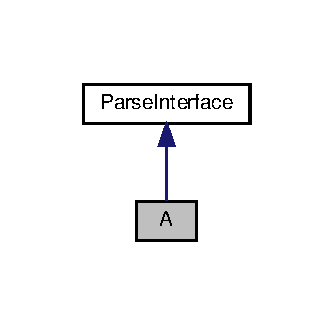
\includegraphics[width=160pt]{classA__inherit__graph}
\end{center}
\end{figure}


Collaboration diagram for A\+:
\nopagebreak
\begin{figure}[H]
\begin{center}
\leavevmode
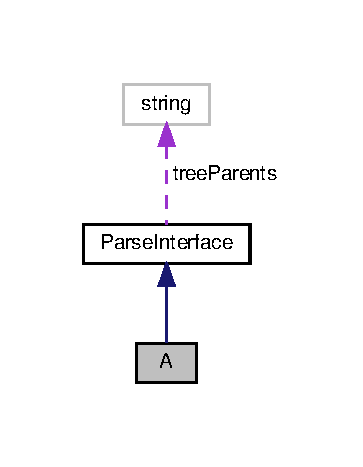
\includegraphics[width=174pt]{classA__coll__graph}
\end{center}
\end{figure}
\subsection*{Public Member Functions}
\begin{DoxyCompactItemize}
\item 
void \hyperlink{classA_a71896ec8a87fd03a725668c503ec64e7}{parse\+Values} ()
\end{DoxyCompactItemize}
\subsection*{Public Attributes}
\begin{DoxyCompactItemize}
\item 
\mbox{\Hypertarget{classA_a2c26c82449219058c4df497d87a20403}\label{classA_a2c26c82449219058c4df497d87a20403}} 
std\+::vector$<$ int $>$ {\bfseries vals}
\end{DoxyCompactItemize}
\subsection*{Additional Inherited Members}


\subsection{Member Function Documentation}
\mbox{\Hypertarget{classA_a71896ec8a87fd03a725668c503ec64e7}\label{classA_a71896ec8a87fd03a725668c503ec64e7}} 
\index{A@{A}!parse\+Values@{parse\+Values}}
\index{parse\+Values@{parse\+Values}!A@{A}}
\subsubsection{\texorpdfstring{parse\+Values()}{parseValues()}}
{\footnotesize\ttfamily void A\+::parse\+Values (\begin{DoxyParamCaption}{ }\end{DoxyParamCaption})\hspace{0.3cm}{\ttfamily [inline]}, {\ttfamily [virtual]}}

Virtual function This is where we select what values we want to parse out of the xml file by calling the parseX functions above. 

Implements \hyperlink{classParseInterface_afca32108192ba0997c9e5a78189b0cbc}{Parse\+Interface}.



The documentation for this class was generated from the following file\+:\begin{DoxyCompactItemize}
\item 
/home/behnam/\+C\+U\+D\+A-\/\+U\+R\+B/xml\+Testing/A.\+h\end{DoxyCompactItemize}

\hypertarget{classArgumentParsing}{}\section{Argument\+Parsing Class Reference}
\label{classArgumentParsing}\index{Argument\+Parsing@{Argument\+Parsing}}


Inheritance diagram for Argument\+Parsing\+:
\nopagebreak
\begin{figure}[H]
\begin{center}
\leavevmode
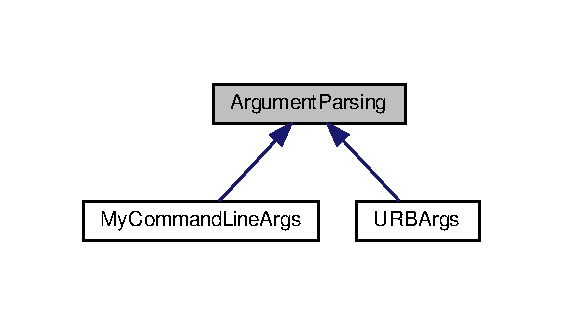
\includegraphics[width=270pt]{classArgumentParsing__inherit__graph}
\end{center}
\end{figure}
\subsection*{Public Types}
\begin{DoxyCompactItemize}
\item 
\mbox{\Hypertarget{classArgumentParsing_afc7b06f169fe65ee044117603822d751}\label{classArgumentParsing_afc7b06f169fe65ee044117603822d751}} 
enum {\bfseries Arg\+Types} \{ \newline
{\bfseries N\+O\+NE}, 
{\bfseries I\+NT}, 
{\bfseries F\+L\+O\+AT}, 
{\bfseries C\+H\+AR}, 
\newline
{\bfseries S\+T\+R\+I\+NG}
 \}
\end{DoxyCompactItemize}
\subsection*{Public Member Functions}
\begin{DoxyCompactItemize}
\item 
\mbox{\Hypertarget{classArgumentParsing_a510548c4ed100184f99970ab68980424}\label{classArgumentParsing_a510548c4ed100184f99970ab68980424}} 
void {\bfseries reg} (const std\+::string \&arg\+Name, const std\+::string \&description, Arg\+Types t, char short\+Arg\+Name=0)
\item 
\mbox{\Hypertarget{classArgumentParsing_af761b06eb7c86d92ffdf590db6ed0b46}\label{classArgumentParsing_af761b06eb7c86d92ffdf590db6ed0b46}} 
int {\bfseries process\+Command\+Line\+Args} (int argc, char $\ast$argv\mbox{[}$\,$\mbox{]})
\item 
\mbox{\Hypertarget{classArgumentParsing_a696c167419b300f3b8161d36234131c7}\label{classArgumentParsing_a696c167419b300f3b8161d36234131c7}} 
bool {\bfseries is\+Set} (const std\+::string \&arg\+Name)
\item 
\mbox{\Hypertarget{classArgumentParsing_a2e9140007f6824a49b0e3fbe658cc3a0}\label{classArgumentParsing_a2e9140007f6824a49b0e3fbe658cc3a0}} 
bool {\bfseries is\+Set} (const std\+::string \&arg\+Name, int \&arg\+Value)
\item 
\mbox{\Hypertarget{classArgumentParsing_ac3572d336f0a9151dd5dc53bd208edb1}\label{classArgumentParsing_ac3572d336f0a9151dd5dc53bd208edb1}} 
bool {\bfseries is\+Set} (const std\+::string \&arg\+Name, float \&arg\+Value)
\item 
\mbox{\Hypertarget{classArgumentParsing_a308f10dbeead11c73b7a1ffbf1c5274a}\label{classArgumentParsing_a308f10dbeead11c73b7a1ffbf1c5274a}} 
bool {\bfseries is\+Set} (const std\+::string \&arg\+Name, char \&arg\+Value)
\item 
\mbox{\Hypertarget{classArgumentParsing_a4e19fd0b5a9a26f106b64decd66610b8}\label{classArgumentParsing_a4e19fd0b5a9a26f106b64decd66610b8}} 
bool {\bfseries is\+Set} (const std\+::string \&arg\+Name, std\+::string \&arg\+Value)
\item 
\mbox{\Hypertarget{classArgumentParsing_a9386d5a547050a15f344b049b167a628}\label{classArgumentParsing_a9386d5a547050a15f344b049b167a628}} 
void {\bfseries print\+Usage} () const
\end{DoxyCompactItemize}
\subsection*{Protected Member Functions}
\begin{DoxyCompactItemize}
\item 
\mbox{\Hypertarget{classArgumentParsing_ab8eaad07d0c28d6e6c9f6a68b7751714}\label{classArgumentParsing_ab8eaad07d0c28d6e6c9f6a68b7751714}} 
int {\bfseries process} (int argc, char $\ast$argv\mbox{[}$\,$\mbox{]})
\end{DoxyCompactItemize}


The documentation for this class was generated from the following files\+:\begin{DoxyCompactItemize}
\item 
/home/behnam/\+C\+U\+D\+A-\/\+U\+R\+B/src/util/Argument\+Parsing.\+h\item 
/home/behnam/\+C\+U\+D\+A-\/\+U\+R\+B/src/util/Argument\+Parsing.\+cpp\end{DoxyCompactItemize}

\hypertarget{classB}{}\section{B Class Reference}
\label{classB}\index{B@{B}}


Inheritance diagram for B\+:
\nopagebreak
\begin{figure}[H]
\begin{center}
\leavevmode
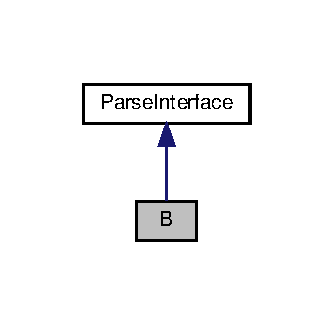
\includegraphics[width=160pt]{classB__inherit__graph}
\end{center}
\end{figure}


Collaboration diagram for B\+:
\nopagebreak
\begin{figure}[H]
\begin{center}
\leavevmode
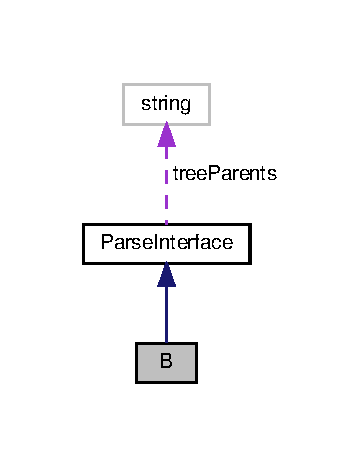
\includegraphics[width=174pt]{classB__coll__graph}
\end{center}
\end{figure}
\subsection*{Public Member Functions}
\begin{DoxyCompactItemize}
\item 
void \hyperlink{classB_abf3989a414e46fb5dd4bd15a279008ab}{parse\+Values} ()
\end{DoxyCompactItemize}
\subsection*{Public Attributes}
\begin{DoxyCompactItemize}
\item 
\mbox{\Hypertarget{classB_ad8f0c5df705d57a962e66430411c71cb}\label{classB_ad8f0c5df705d57a962e66430411c71cb}} 
int {\bfseries num\+As}
\item 
\mbox{\Hypertarget{classB_a7e3c14c4eb5bd4cb1543ea4832efc37f}\label{classB_a7e3c14c4eb5bd4cb1543ea4832efc37f}} 
std\+::vector$<$ \hyperlink{classA}{A} $\ast$ $>$ {\bfseries a\+Vals}
\end{DoxyCompactItemize}
\subsection*{Additional Inherited Members}


\subsection{Member Function Documentation}
\mbox{\Hypertarget{classB_abf3989a414e46fb5dd4bd15a279008ab}\label{classB_abf3989a414e46fb5dd4bd15a279008ab}} 
\index{B@{B}!parse\+Values@{parse\+Values}}
\index{parse\+Values@{parse\+Values}!B@{B}}
\subsubsection{\texorpdfstring{parse\+Values()}{parseValues()}}
{\footnotesize\ttfamily void B\+::parse\+Values (\begin{DoxyParamCaption}{ }\end{DoxyParamCaption})\hspace{0.3cm}{\ttfamily [inline]}, {\ttfamily [virtual]}}

Virtual function This is where we select what values we want to parse out of the xml file by calling the parseX functions above. 

Implements \hyperlink{classParseInterface_afca32108192ba0997c9e5a78189b0cbc}{Parse\+Interface}.



The documentation for this class was generated from the following file\+:\begin{DoxyCompactItemize}
\item 
/home/behnam/\+C\+U\+D\+A-\/\+U\+R\+B/xml\+Testing/B.\+h\end{DoxyCompactItemize}

\hypertarget{classBuilding}{}\section{Building Class Reference}
\label{classBuilding}\index{Building@{Building}}


Inheritance diagram for Building\+:
\nopagebreak
\begin{figure}[H]
\begin{center}
\leavevmode
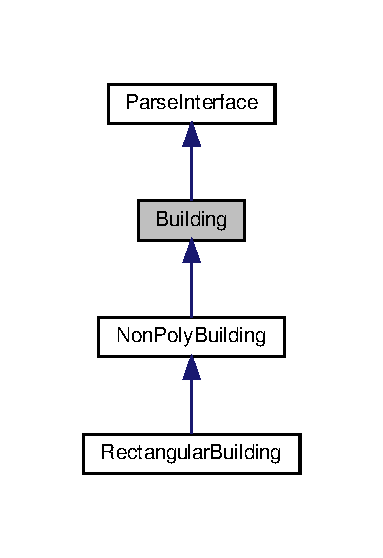
\includegraphics[width=184pt]{classBuilding__inherit__graph}
\end{center}
\end{figure}


Collaboration diagram for Building\+:
\nopagebreak
\begin{figure}[H]
\begin{center}
\leavevmode
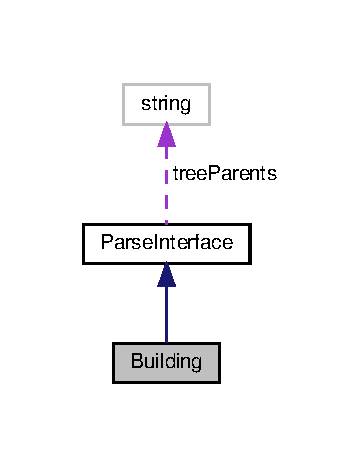
\includegraphics[width=174pt]{classBuilding__coll__graph}
\end{center}
\end{figure}
\subsection*{Public Member Functions}
\begin{DoxyCompactItemize}
\item 
virtual void \hyperlink{classBuilding_a7782e7933a009fcfee4d186e62d34b43}{parse\+Values} ()=0
\end{DoxyCompactItemize}
\subsection*{Public Attributes}
\begin{DoxyCompactItemize}
\item 
\mbox{\Hypertarget{classBuilding_a29af720d04ca4fafa0881ca73f7ce54b}\label{classBuilding_a29af720d04ca4fafa0881ca73f7ce54b}} 
int {\bfseries group\+ID}
\item 
\mbox{\Hypertarget{classBuilding_a35ee8dac0d2288329bb10cb78af996a1}\label{classBuilding_a35ee8dac0d2288329bb10cb78af996a1}} 
int {\bfseries building\+Type}
\item 
\mbox{\Hypertarget{classBuilding_aa8753ccee0f2dd6144c418e9cf08e41e}\label{classBuilding_aa8753ccee0f2dd6144c418e9cf08e41e}} 
int {\bfseries building\+Geometry}
\item 
\mbox{\Hypertarget{classBuilding_a0e34228cdc88c79f58d0cee0f445965c}\label{classBuilding_a0e34228cdc88c79f58d0cee0f445965c}} 
float {\bfseries H}
\item 
\mbox{\Hypertarget{classBuilding_a23e46ffbb553247f8c29f59c4e97a8eb}\label{classBuilding_a23e46ffbb553247f8c29f59c4e97a8eb}} 
float {\bfseries base\+Height}
\item 
\mbox{\Hypertarget{classBuilding_a7cf1f72edd89f924da35292d923254c9}\label{classBuilding_a7cf1f72edd89f924da35292d923254c9}} 
float {\bfseries base\+Height\+Actual}
\item 
\mbox{\Hypertarget{classBuilding_aec20efa3786ccaabe32efbda691bc590}\label{classBuilding_aec20efa3786ccaabe32efbda691bc590}} 
int {\bfseries i\+\_\+\+Start}
\item 
\mbox{\Hypertarget{classBuilding_a9db428412881d49d12652a324c7cfb4e}\label{classBuilding_a9db428412881d49d12652a324c7cfb4e}} 
int {\bfseries i\+\_\+end}
\item 
\mbox{\Hypertarget{classBuilding_a00f6578807f04108df0495ded977fa63}\label{classBuilding_a00f6578807f04108df0495ded977fa63}} 
int {\bfseries j\+\_\+start}
\item 
\mbox{\Hypertarget{classBuilding_ab64d69b96f6a7b2378638e4b83bcf87e}\label{classBuilding_ab64d69b96f6a7b2378638e4b83bcf87e}} 
int {\bfseries j\+\_\+end}
\item 
\mbox{\Hypertarget{classBuilding_a6fc8960b3f733c6b74d80738692e5b6f}\label{classBuilding_a6fc8960b3f733c6b74d80738692e5b6f}} 
int {\bfseries k\+\_\+start}
\item 
\mbox{\Hypertarget{classBuilding_add46553b9552e66fce86eadd3d6b477f}\label{classBuilding_add46553b9552e66fce86eadd3d6b477f}} 
int {\bfseries k\+\_\+end}
\item 
\mbox{\Hypertarget{classBuilding_af6356b3fb49ae82467c157cbfcb385ef}\label{classBuilding_af6356b3fb49ae82467c157cbfcb385ef}} 
int {\bfseries i\+\_\+cut\+\_\+start}
\item 
\mbox{\Hypertarget{classBuilding_afa5671c0e1422af4f0c17f9a252c3eb0}\label{classBuilding_afa5671c0e1422af4f0c17f9a252c3eb0}} 
int {\bfseries i\+\_\+cut\+\_\+end}
\item 
\mbox{\Hypertarget{classBuilding_a329a8d554ca99ae2b04ed29b85372a3e}\label{classBuilding_a329a8d554ca99ae2b04ed29b85372a3e}} 
int {\bfseries j\+\_\+cut\+\_\+start}
\item 
\mbox{\Hypertarget{classBuilding_a51d4d706d25829c43b348e0a75667bb3}\label{classBuilding_a51d4d706d25829c43b348e0a75667bb3}} 
int {\bfseries j\+\_\+cut\+\_\+end}
\item 
\mbox{\Hypertarget{classBuilding_a0a5fec2433094e4d795aebdb68c3051c}\label{classBuilding_a0a5fec2433094e4d795aebdb68c3051c}} 
int {\bfseries k\+\_\+cut\+\_\+end}
\end{DoxyCompactItemize}
\subsection*{Additional Inherited Members}


\subsection{Member Function Documentation}
\mbox{\Hypertarget{classBuilding_a7782e7933a009fcfee4d186e62d34b43}\label{classBuilding_a7782e7933a009fcfee4d186e62d34b43}} 
\index{Building@{Building}!parse\+Values@{parse\+Values}}
\index{parse\+Values@{parse\+Values}!Building@{Building}}
\subsubsection{\texorpdfstring{parse\+Values()}{parseValues()}}
{\footnotesize\ttfamily virtual void Building\+::parse\+Values (\begin{DoxyParamCaption}{ }\end{DoxyParamCaption})\hspace{0.3cm}{\ttfamily [pure virtual]}}

Virtual function This is where we select what values we want to parse out of the xml file by calling the parseX functions above. 

Implements \hyperlink{classParseInterface_afca32108192ba0997c9e5a78189b0cbc}{Parse\+Interface}.



Implemented in \hyperlink{classRectangularBuilding_adbc6b832c817fc06f9bc2e51561a7e81}{Rectangular\+Building}, and \hyperlink{classNonPolyBuilding_ace133756e0233d75b434fec5273b4414}{Non\+Poly\+Building}.



The documentation for this class was generated from the following file\+:\begin{DoxyCompactItemize}
\item 
/home/behnam/\+C\+U\+D\+A-\/\+U\+R\+B/src/Building.\+h\end{DoxyCompactItemize}

\hypertarget{classBuildings}{}\section{Buildings Class Reference}
\label{classBuildings}\index{Buildings@{Buildings}}


Inheritance diagram for Buildings\+:
\nopagebreak
\begin{figure}[H]
\begin{center}
\leavevmode
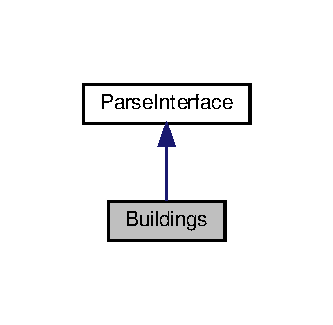
\includegraphics[width=160pt]{classBuildings__inherit__graph}
\end{center}
\end{figure}


Collaboration diagram for Buildings\+:
\nopagebreak
\begin{figure}[H]
\begin{center}
\leavevmode
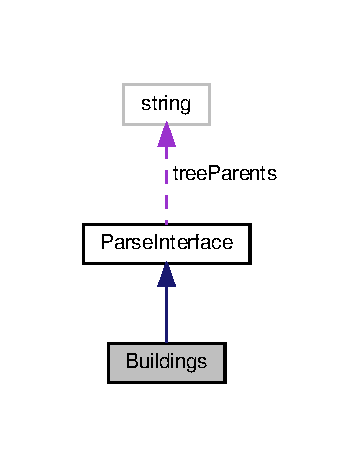
\includegraphics[width=174pt]{classBuildings__coll__graph}
\end{center}
\end{figure}
\subsection*{Public Member Functions}
\begin{DoxyCompactItemize}
\item 
virtual void \hyperlink{classBuildings_a97851dd190977ba999ecb1f50481c400}{parse\+Values} ()
\end{DoxyCompactItemize}
\subsection*{Public Attributes}
\begin{DoxyCompactItemize}
\item 
\mbox{\Hypertarget{classBuildings_ad813fd3b4a16573db8053b37d5b97bda}\label{classBuildings_ad813fd3b4a16573db8053b37d5b97bda}} 
int {\bfseries num\+Buildings}
\item 
\mbox{\Hypertarget{classBuildings_af2ce540b40f5555f705800187e34a8b9}\label{classBuildings_af2ce540b40f5555f705800187e34a8b9}} 
int {\bfseries num\+Polygon\+Nodes}
\item 
\mbox{\Hypertarget{classBuildings_a50977969dd40837e447d794a2bc07238}\label{classBuildings_a50977969dd40837e447d794a2bc07238}} 
std\+::vector$<$ \hyperlink{classBuilding}{Building} $\ast$ $>$ {\bfseries buildings}
\item 
\mbox{\Hypertarget{classBuildings_a250aa6acd2da48a13193ff4412536115}\label{classBuildings_a250aa6acd2da48a13193ff4412536115}} 
float {\bfseries wall\+Roughness}
\end{DoxyCompactItemize}
\subsection*{Additional Inherited Members}


\subsection{Member Function Documentation}
\mbox{\Hypertarget{classBuildings_a97851dd190977ba999ecb1f50481c400}\label{classBuildings_a97851dd190977ba999ecb1f50481c400}} 
\index{Buildings@{Buildings}!parse\+Values@{parse\+Values}}
\index{parse\+Values@{parse\+Values}!Buildings@{Buildings}}
\subsubsection{\texorpdfstring{parse\+Values()}{parseValues()}}
{\footnotesize\ttfamily virtual void Buildings\+::parse\+Values (\begin{DoxyParamCaption}{ }\end{DoxyParamCaption})\hspace{0.3cm}{\ttfamily [inline]}, {\ttfamily [virtual]}}

Virtual function This is where we select what values we want to parse out of the xml file by calling the parseX functions above. 

Implements \hyperlink{classParseInterface_afca32108192ba0997c9e5a78189b0cbc}{Parse\+Interface}.



The documentation for this class was generated from the following file\+:\begin{DoxyCompactItemize}
\item 
/home/behnam/\+C\+U\+D\+A-\/\+U\+R\+B/src/Buildings.\+h\end{DoxyCompactItemize}

\hypertarget{classBVH}{}\section{B\+VH Class Reference}
\label{classBVH}\index{B\+VH@{B\+VH}}
\subsection*{Public Member Functions}
\begin{DoxyCompactItemize}
\item 
\mbox{\Hypertarget{classBVH_aad5f857a15fbe4fc58c7ecdc38ed8e6c}\label{classBVH_aad5f857a15fbe4fc58c7ecdc38ed8e6c}} 
{\bfseries B\+VH} (\hyperlink{classBVH}{B\+VH} $\ast$l, \hyperlink{classBVH}{B\+VH} $\ast$r)
\item 
\mbox{\Hypertarget{classBVH_aa937fa954ef0afb7918585383a1b7d45}\label{classBVH_aa937fa954ef0afb7918585383a1b7d45}} 
{\bfseries B\+VH} (\hyperlink{classTriangle}{Triangle} $\ast$t)
\item 
\mbox{\Hypertarget{classBVH_a52aae90a6245e0d144bfb43cb118eb6e}\label{classBVH_a52aae90a6245e0d144bfb43cb118eb6e}} 
{\bfseries B\+VH} (std\+::vector$<$ \hyperlink{classBVH}{B\+VH} $\ast$$>$ m, int height)
\item 
\mbox{\Hypertarget{classBVH_ad0c58e6a547f0cb238f23d1f50bb367a}\label{classBVH_ad0c58e6a547f0cb238f23d1f50bb367a}} 
float {\bfseries height\+To\+Tri} (float x, float y)
\end{DoxyCompactItemize}
\subsection*{Static Public Member Functions}
\begin{DoxyCompactItemize}
\item 
\mbox{\Hypertarget{classBVH_a039d56c9683671bf2526034d855ca53c}\label{classBVH_a039d56c9683671bf2526034d855ca53c}} 
static \hyperlink{classBVH}{B\+VH} $\ast$ {\bfseries create\+B\+VH} (const std\+::vector$<$ \hyperlink{classTriangle}{Triangle} $\ast$$>$ tris)
\end{DoxyCompactItemize}
\subsection*{Public Attributes}
\begin{DoxyCompactItemize}
\item 
\mbox{\Hypertarget{classBVH_a30785206fdaa43dd6bb15d6bc2ebde1b}\label{classBVH_a30785206fdaa43dd6bb15d6bc2ebde1b}} 
float {\bfseries xmin}
\item 
\mbox{\Hypertarget{classBVH_a0365945971422100f7201678a2f90704}\label{classBVH_a0365945971422100f7201678a2f90704}} 
float {\bfseries xmax}
\item 
\mbox{\Hypertarget{classBVH_a6806c8211fc8f5c590131e14bb45805e}\label{classBVH_a6806c8211fc8f5c590131e14bb45805e}} 
float {\bfseries ymin}
\item 
\mbox{\Hypertarget{classBVH_a15a7b2213cc41a5f349a6a1d761303d6}\label{classBVH_a15a7b2213cc41a5f349a6a1d761303d6}} 
float {\bfseries ymax}
\item 
\mbox{\Hypertarget{classBVH_a9d494f2331680f38832144546a99260c}\label{classBVH_a9d494f2331680f38832144546a99260c}} 
float {\bfseries zmin}
\item 
\mbox{\Hypertarget{classBVH_a5c5a3f9b16fc8f9af6ed2fcc53d58f53}\label{classBVH_a5c5a3f9b16fc8f9af6ed2fcc53d58f53}} 
float {\bfseries zmax}
\end{DoxyCompactItemize}


The documentation for this class was generated from the following files\+:\begin{DoxyCompactItemize}
\item 
/home/behnam/\+C\+U\+D\+A-\/\+U\+R\+B/src/B\+V\+H.\+h\item 
/home/behnam/\+C\+U\+D\+A-\/\+U\+R\+B/src/B\+V\+H.\+cpp\end{DoxyCompactItemize}

\hypertarget{classC}{}\section{C Class Reference}
\label{classC}\index{C@{C}}


Inheritance diagram for C\+:
\nopagebreak
\begin{figure}[H]
\begin{center}
\leavevmode
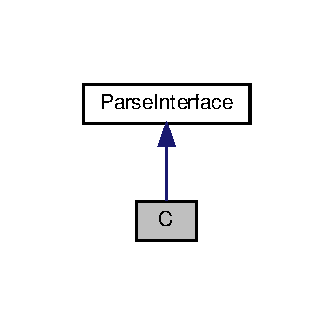
\includegraphics[width=160pt]{classC__inherit__graph}
\end{center}
\end{figure}


Collaboration diagram for C\+:
\nopagebreak
\begin{figure}[H]
\begin{center}
\leavevmode
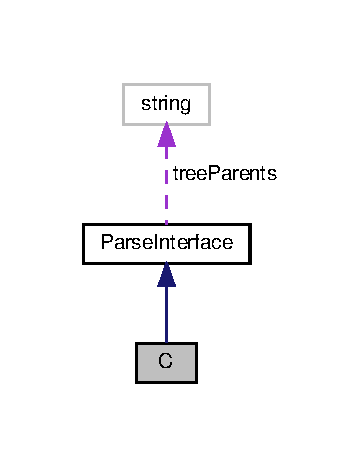
\includegraphics[width=174pt]{classC__coll__graph}
\end{center}
\end{figure}
\subsection*{Public Member Functions}
\begin{DoxyCompactItemize}
\item 
void \hyperlink{classC_a7f8b8fa8187ab2f50ca999ae9a1687d7}{parse\+Values} ()
\end{DoxyCompactItemize}
\subsection*{Public Attributes}
\begin{DoxyCompactItemize}
\item 
\mbox{\Hypertarget{classC_acd8eedda62e4ea6c74b7e0b59245a357}\label{classC_acd8eedda62e4ea6c74b7e0b59245a357}} 
float {\bfseries y}
\item 
\mbox{\Hypertarget{classC_a644bc4405a602578b65e83d317a2f3eb}\label{classC_a644bc4405a602578b65e83d317a2f3eb}} 
int {\bfseries x}
\end{DoxyCompactItemize}
\subsection*{Additional Inherited Members}


\subsection{Member Function Documentation}
\mbox{\Hypertarget{classC_a7f8b8fa8187ab2f50ca999ae9a1687d7}\label{classC_a7f8b8fa8187ab2f50ca999ae9a1687d7}} 
\index{C@{C}!parse\+Values@{parse\+Values}}
\index{parse\+Values@{parse\+Values}!C@{C}}
\subsubsection{\texorpdfstring{parse\+Values()}{parseValues()}}
{\footnotesize\ttfamily void C\+::parse\+Values (\begin{DoxyParamCaption}{ }\end{DoxyParamCaption})\hspace{0.3cm}{\ttfamily [inline]}, {\ttfamily [virtual]}}

Virtual function This is where we select what values we want to parse out of the xml file by calling the parseX functions above. 

Implements \hyperlink{classParseInterface_afca32108192ba0997c9e5a78189b0cbc}{Parse\+Interface}.



The documentation for this class was generated from the following file\+:\begin{DoxyCompactItemize}
\item 
/home/behnam/\+C\+U\+D\+A-\/\+U\+R\+B/xml\+Testing/C.\+h\end{DoxyCompactItemize}

\hypertarget{classCell}{}\section{Cell Class Reference}
\label{classCell}\index{Cell@{Cell}}
\subsection*{Public Member Functions}
\begin{DoxyCompactItemize}
\item 
\mbox{\Hypertarget{classCell_aa874e7ad3c62688dceed3a515466b72a}\label{classCell_aa874e7ad3c62688dceed3a515466b72a}} 
bool {\bfseries get\+Is\+Air} ()
\item 
\mbox{\Hypertarget{classCell_a13fba362f6cf077c9aae6b76cb804821}\label{classCell_a13fba362f6cf077c9aae6b76cb804821}} 
bool {\bfseries get\+Is\+Terrain} ()
\item 
\mbox{\Hypertarget{classCell_a5ab69f678e05c66388f1a7c204425eb2}\label{classCell_a5ab69f678e05c66388f1a7c204425eb2}} 
bool {\bfseries get\+Is\+Cut\+Cell} ()
\item 
\mbox{\Hypertarget{classCell_ae367fdf7c82557dc6a545cf3e364eb77}\label{classCell_ae367fdf7c82557dc6a545cf3e364eb77}} 
std\+::vector$<$ \hyperlink{classVector3}{Vector3}$<$ float $>$ $>$ {\bfseries get\+Terrain\+Points} ()
\item 
\mbox{\Hypertarget{classCell_a605ab530a9945f4dde5e669c0aed42a7}\label{classCell_a605ab530a9945f4dde5e669c0aed42a7}} 
{\bfseries Cell} (int type\+\_\+\+CT)
\item 
\mbox{\Hypertarget{classCell_a09ab8599cd1e5d35231870587dbbaaea}\label{classCell_a09ab8599cd1e5d35231870587dbbaaea}} 
{\bfseries Cell} (std\+::vector$<$ \hyperlink{classVector3}{Vector3}$<$ float $>$ $>$ points)
\end{DoxyCompactItemize}


The documentation for this class was generated from the following files\+:\begin{DoxyCompactItemize}
\item 
/home/behnam/\+C\+U\+D\+A-\/\+U\+R\+B/src/Cell.\+h\item 
/home/behnam/\+C\+U\+D\+A-\/\+U\+R\+B/src/Cell.\+cpp\end{DoxyCompactItemize}

\hypertarget{classCPUSolver}{}\section{C\+P\+U\+Solver Class Reference}
\label{classCPUSolver}\index{C\+P\+U\+Solver@{C\+P\+U\+Solver}}


Inheritance diagram for C\+P\+U\+Solver\+:
\nopagebreak
\begin{figure}[H]
\begin{center}
\leavevmode
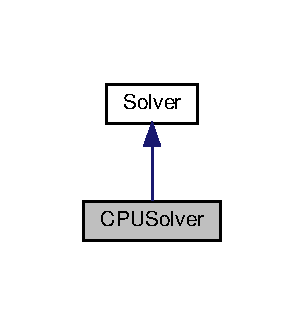
\includegraphics[width=146pt]{classCPUSolver__inherit__graph}
\end{center}
\end{figure}


Collaboration diagram for C\+P\+U\+Solver\+:
\nopagebreak
\begin{figure}[H]
\begin{center}
\leavevmode
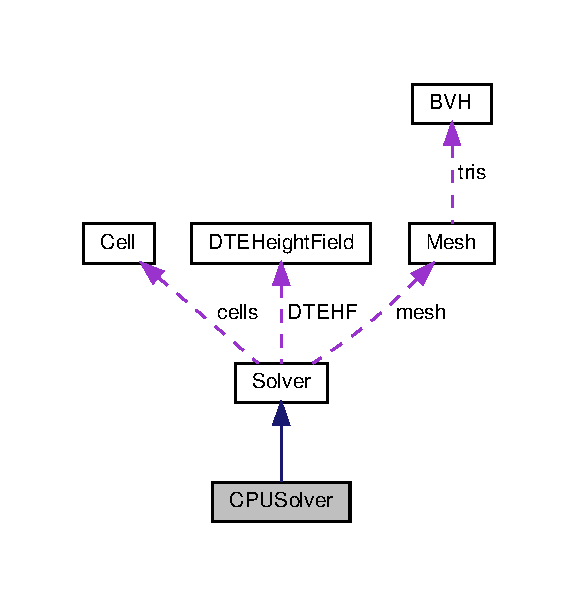
\includegraphics[width=278pt]{classCPUSolver__coll__graph}
\end{center}
\end{figure}
\subsection*{Public Member Functions}
\begin{DoxyCompactItemize}
\item 
\mbox{\Hypertarget{classCPUSolver_a681ee9c01d35cff794f31726cf0ec044}\label{classCPUSolver_a681ee9c01d35cff794f31726cf0ec044}} 
{\bfseries C\+P\+U\+Solver} (\hyperlink{classURBInputData}{U\+R\+B\+Input\+Data} $\ast$U\+ID, \hyperlink{classDTEHeightField}{D\+T\+E\+Height\+Field} $\ast$D\+T\+E\+HF)
\item 
virtual void \hyperlink{classCPUSolver_aaf3f4e100bcb96430461c935aaab23d1}{solve} (\hyperlink{classNetCDFData}{Net\+C\+D\+F\+Data} $\ast$netcdf\+Dat, bool solve\+Wind)
\end{DoxyCompactItemize}
\subsection*{Additional Inherited Members}


\subsection{Member Function Documentation}
\mbox{\Hypertarget{classCPUSolver_aaf3f4e100bcb96430461c935aaab23d1}\label{classCPUSolver_aaf3f4e100bcb96430461c935aaab23d1}} 
\index{C\+P\+U\+Solver@{C\+P\+U\+Solver}!solve@{solve}}
\index{solve@{solve}!C\+P\+U\+Solver@{C\+P\+U\+Solver}}
\subsubsection{\texorpdfstring{solve()}{solve()}}
{\footnotesize\ttfamily void C\+P\+U\+Solver\+::solve (\begin{DoxyParamCaption}\item[{\hyperlink{classNetCDFData}{Net\+C\+D\+F\+Data} $\ast$}]{netcdf\+Dat,  }\item[{bool}]{solve\+Wind }\end{DoxyParamCaption})\hspace{0.3cm}{\ttfamily [virtual]}}

located in \hyperlink{RectangularBuilding_8h_source}{Rectangular\+Building.\+h}

Lineralized index for cell centered values

Lineralized index for cell faced values

Set velocity inside the building to zero

Set velocity inside the building to zero

Set velocity inside the building to zero

Lineralized index for cell centered values

Lineralized index for cell faced values

Calculate divergence of initial velocity field

New boundary condition implementation

Lineralized index for cell centered values

Save previous iteration values for error calculation

Lineralized index for cell centered values

Lineralized index for cell centered values

S\+OR formulation

Mirror boundary condition (lambda (=0) = lambda (=1))

Lineralized index for cell centered values

Reset error value before error calculation

Error calculation

Lineralized index for cell centered values

Lineralized index for cell faced values

Update velocity field using Euler equations

Lineralized index for cell centered values

Lineralized index for cell faced values

Setting velocity field inside the building to zero

Lineralized index for cell centered values

Lineralized index for cell faced values

Declare cell center positions

Location of cell centers in x-\/dir

Location of cell centers in y-\/dir

Location of cell centers in z-\/dir

Declare output velocity field arrays

Lineralized index for cell faced values

Lineralized index for cell centered values

Lineralized index for cell faced values

Lineralized index for cell centered values

Lineralized index for cell faced values

Location of cell centers in x-\/dir

Location of cell centers in y-\/dir

Location of cell centers in z-\/dir 

Implements \hyperlink{classSolver}{Solver}.



The documentation for this class was generated from the following files\+:\begin{DoxyCompactItemize}
\item 
/home/behnam/\+C\+U\+D\+A-\/\+U\+R\+B/src/C\+P\+U\+Solver.\+h\item 
/home/behnam/\+C\+U\+D\+A-\/\+U\+R\+B/src/C\+P\+U\+Solver.\+cpp\end{DoxyCompactItemize}

\hypertarget{classD}{}\section{D Class Reference}
\label{classD}\index{D@{D}}


Inheritance diagram for D\+:
\nopagebreak
\begin{figure}[H]
\begin{center}
\leavevmode
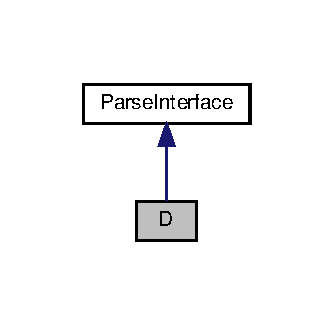
\includegraphics[width=160pt]{classD__inherit__graph}
\end{center}
\end{figure}


Collaboration diagram for D\+:
\nopagebreak
\begin{figure}[H]
\begin{center}
\leavevmode
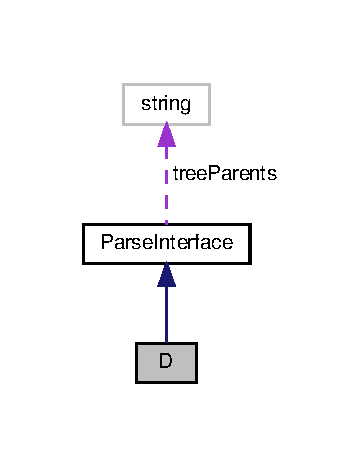
\includegraphics[width=174pt]{classD__coll__graph}
\end{center}
\end{figure}
\subsection*{Public Member Functions}
\begin{DoxyCompactItemize}
\item 
void \hyperlink{classD_afd52a3aa7a7e9047386deb6aeb796b2a}{parse\+Values} ()
\end{DoxyCompactItemize}
\subsection*{Public Attributes}
\begin{DoxyCompactItemize}
\item 
\mbox{\Hypertarget{classD_ad1756e0458999b2ba792d35d2715cb83}\label{classD_ad1756e0458999b2ba792d35d2715cb83}} 
std\+::vector$<$ \hyperlink{classP}{P} $\ast$ $>$ {\bfseries p\+Vars}
\end{DoxyCompactItemize}
\subsection*{Additional Inherited Members}


\subsection{Member Function Documentation}
\mbox{\Hypertarget{classD_afd52a3aa7a7e9047386deb6aeb796b2a}\label{classD_afd52a3aa7a7e9047386deb6aeb796b2a}} 
\index{D@{D}!parse\+Values@{parse\+Values}}
\index{parse\+Values@{parse\+Values}!D@{D}}
\subsubsection{\texorpdfstring{parse\+Values()}{parseValues()}}
{\footnotesize\ttfamily void D\+::parse\+Values (\begin{DoxyParamCaption}{ }\end{DoxyParamCaption})\hspace{0.3cm}{\ttfamily [inline]}, {\ttfamily [virtual]}}

Virtual function This is where we select what values we want to parse out of the xml file by calling the parseX functions above. 

Implements \hyperlink{classParseInterface_afca32108192ba0997c9e5a78189b0cbc}{Parse\+Interface}.



The documentation for this class was generated from the following file\+:\begin{DoxyCompactItemize}
\item 
/home/behnam/\+C\+U\+D\+A-\/\+U\+R\+B/xml\+Testing/D.\+h\end{DoxyCompactItemize}

\hypertarget{classDTEHeightField}{}\section{D\+T\+E\+Height\+Field Class Reference}
\label{classDTEHeightField}\index{D\+T\+E\+Height\+Field@{D\+T\+E\+Height\+Field}}
\subsection*{Public Member Functions}
\begin{DoxyCompactItemize}
\item 
\mbox{\Hypertarget{classDTEHeightField_aebd33cfb7c7ce087e341ceecea15a358}\label{classDTEHeightField_aebd33cfb7c7ce087e341ceecea15a358}} 
{\bfseries D\+T\+E\+Height\+Field} (const std\+::string \&filename, double cell\+Size\+XN, double cell\+Size\+YN)
\item 
\mbox{\Hypertarget{classDTEHeightField_a167ff2b1b9e969f04f2269b268ca7ba5}\label{classDTEHeightField_a167ff2b1b9e969f04f2269b268ca7ba5}} 
std\+::vector$<$ \hyperlink{classTriangle}{Triangle} $\ast$ $>$ {\bfseries get\+Tris} ()
\item 
\mbox{\Hypertarget{classDTEHeightField_a5890b28c0c907972103e8e0317455800}\label{classDTEHeightField_a5890b28c0c907972103e8e0317455800}} 
void {\bfseries set\+Domain} (\hyperlink{classVector3}{Vector3}$<$ int $>$ $\ast$domain, \hyperlink{classVector3}{Vector3}$<$ float $>$ $\ast$grid)
\item 
\mbox{\Hypertarget{classDTEHeightField_a39ebb3ac406dadfa20d010cd9f015131}\label{classDTEHeightField_a39ebb3ac406dadfa20d010cd9f015131}} 
void {\bfseries output\+O\+BJ} (std\+::string s)
\item 
\mbox{\Hypertarget{classDTEHeightField_ae8c7ad231888af85cbe4e4bb19dd5474}\label{classDTEHeightField_ae8c7ad231888af85cbe4e4bb19dd5474}} 
std\+::vector$<$ int $>$ {\bfseries set\+Cells} (\hyperlink{classCell}{Cell} $\ast$cells, int nx, int ny, int nz, float dx, float dy, float dz)
\end{DoxyCompactItemize}


The documentation for this class was generated from the following files\+:\begin{DoxyCompactItemize}
\item 
/home/behnam/\+C\+U\+D\+A-\/\+U\+R\+B/src/D\+T\+E\+Height\+Field.\+h\item 
/home/behnam/\+C\+U\+D\+A-\/\+U\+R\+B/src/D\+T\+E\+Height\+Field.\+cpp\end{DoxyCompactItemize}

\hypertarget{classDynamicParallelism}{}\section{Dynamic\+Parallelism Class Reference}
\label{classDynamicParallelism}\index{Dynamic\+Parallelism@{Dynamic\+Parallelism}}


Inheritance diagram for Dynamic\+Parallelism\+:
\nopagebreak
\begin{figure}[H]
\begin{center}
\leavevmode
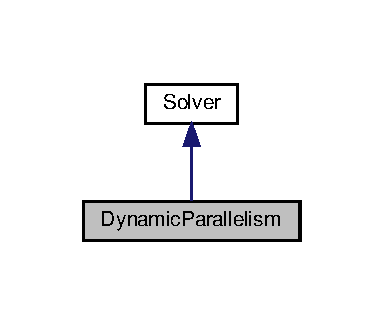
\includegraphics[width=184pt]{classDynamicParallelism__inherit__graph}
\end{center}
\end{figure}


Collaboration diagram for Dynamic\+Parallelism\+:
\nopagebreak
\begin{figure}[H]
\begin{center}
\leavevmode
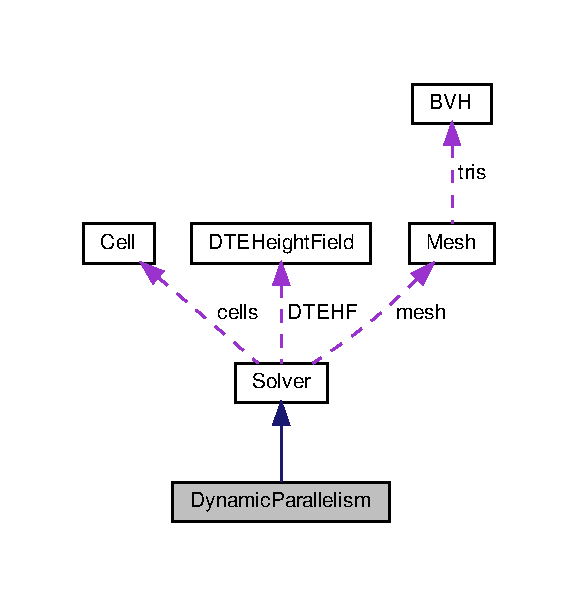
\includegraphics[width=278pt]{classDynamicParallelism__coll__graph}
\end{center}
\end{figure}
\subsection*{Public Member Functions}
\begin{DoxyCompactItemize}
\item 
\mbox{\Hypertarget{classDynamicParallelism_acc31e51a0f4a462d60d53053abfcbf66}\label{classDynamicParallelism_acc31e51a0f4a462d60d53053abfcbf66}} 
{\bfseries Dynamic\+Parallelism} (\hyperlink{classURBInputData}{U\+R\+B\+Input\+Data} $\ast$U\+ID, \hyperlink{classDTEHeightField}{D\+T\+E\+Height\+Field} $\ast$D\+T\+E\+HF)
\item 
\mbox{\Hypertarget{classDynamicParallelism_a43c7a33a4853ef887c78c3d28b9caaf5}\label{classDynamicParallelism_a43c7a33a4853ef887c78c3d28b9caaf5}} 
virtual void {\bfseries solve} (\hyperlink{classNetCDFData}{Net\+C\+D\+F\+Data} $\ast$netcdf\+Dat, bool solve\+Wind)
\end{DoxyCompactItemize}
\subsection*{Additional Inherited Members}


The documentation for this class was generated from the following file\+:\begin{DoxyCompactItemize}
\item 
/home/behnam/\+C\+U\+D\+A-\/\+U\+R\+B/src/Dynamic\+Parallelism.\+h\end{DoxyCompactItemize}

\hypertarget{classFileOptions}{}\section{File\+Options Class Reference}
\label{classFileOptions}\index{File\+Options@{File\+Options}}


Inheritance diagram for File\+Options\+:
\nopagebreak
\begin{figure}[H]
\begin{center}
\leavevmode
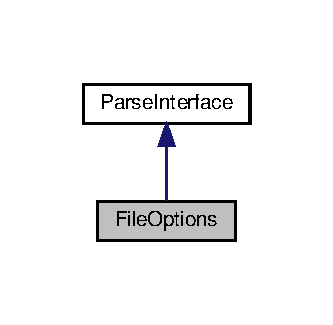
\includegraphics[width=160pt]{classFileOptions__inherit__graph}
\end{center}
\end{figure}


Collaboration diagram for File\+Options\+:
\nopagebreak
\begin{figure}[H]
\begin{center}
\leavevmode
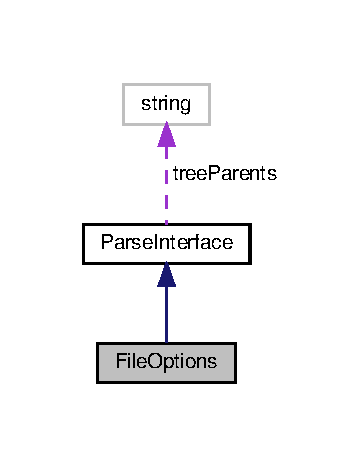
\includegraphics[width=174pt]{classFileOptions__coll__graph}
\end{center}
\end{figure}
\subsection*{Public Member Functions}
\begin{DoxyCompactItemize}
\item 
virtual void \hyperlink{classFileOptions_aca2f6304ed7d1fdde5c6c392d7fd11b9}{parse\+Values} ()
\end{DoxyCompactItemize}
\subsection*{Public Attributes}
\begin{DoxyCompactItemize}
\item 
\mbox{\Hypertarget{classFileOptions_a8b18bf8ae9f804ac81ca8b87e0f52c7a}\label{classFileOptions_a8b18bf8ae9f804ac81ca8b87e0f52c7a}} 
int {\bfseries output\+Format}
\item 
\mbox{\Hypertarget{classFileOptions_aa016071f4f488afc701c2ac87f21aefb}\label{classFileOptions_aa016071f4f488afc701c2ac87f21aefb}} 
bool {\bfseries mass\+Conserved\+Flag}
\item 
\mbox{\Hypertarget{classFileOptions_abe6b2ae12234d7976ee42b8b03721a95}\label{classFileOptions_abe6b2ae12234d7976ee42b8b03721a95}} 
bool {\bfseries sensor\+Velocity\+Flag}
\item 
\mbox{\Hypertarget{classFileOptions_af3e20b4b957b31526d8f0fcb0e506ad8}\label{classFileOptions_af3e20b4b957b31526d8f0fcb0e506ad8}} 
bool {\bfseries staggerd\+Velocity\+Flag}
\end{DoxyCompactItemize}
\subsection*{Additional Inherited Members}


\subsection{Member Function Documentation}
\mbox{\Hypertarget{classFileOptions_aca2f6304ed7d1fdde5c6c392d7fd11b9}\label{classFileOptions_aca2f6304ed7d1fdde5c6c392d7fd11b9}} 
\index{File\+Options@{File\+Options}!parse\+Values@{parse\+Values}}
\index{parse\+Values@{parse\+Values}!File\+Options@{File\+Options}}
\subsubsection{\texorpdfstring{parse\+Values()}{parseValues()}}
{\footnotesize\ttfamily virtual void File\+Options\+::parse\+Values (\begin{DoxyParamCaption}{ }\end{DoxyParamCaption})\hspace{0.3cm}{\ttfamily [inline]}, {\ttfamily [virtual]}}

Virtual function This is where we select what values we want to parse out of the xml file by calling the parseX functions above. 

Implements \hyperlink{classParseInterface_afca32108192ba0997c9e5a78189b0cbc}{Parse\+Interface}.



The documentation for this class was generated from the following file\+:\begin{DoxyCompactItemize}
\item 
/home/behnam/\+C\+U\+D\+A-\/\+U\+R\+B/src/File\+Options.\+h\end{DoxyCompactItemize}

\hypertarget{classGeneralInputData}{}\section{General\+Input\+Data Class Reference}
\label{classGeneralInputData}\index{General\+Input\+Data@{General\+Input\+Data}}


Inheritance diagram for General\+Input\+Data\+:
\nopagebreak
\begin{figure}[H]
\begin{center}
\leavevmode
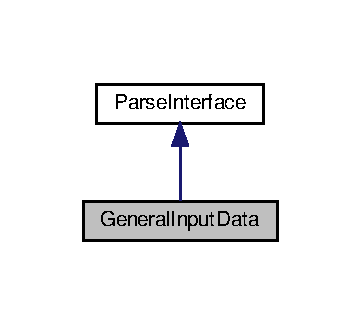
\includegraphics[width=173pt]{classGeneralInputData__inherit__graph}
\end{center}
\end{figure}


Collaboration diagram for General\+Input\+Data\+:
\nopagebreak
\begin{figure}[H]
\begin{center}
\leavevmode
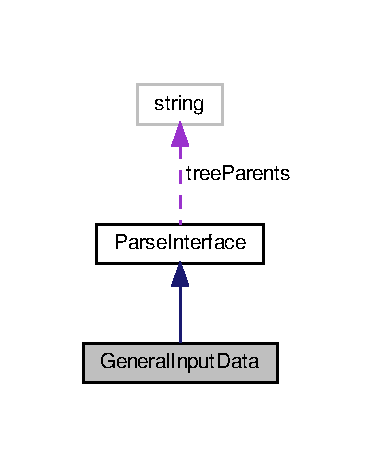
\includegraphics[width=181pt]{classGeneralInputData__coll__graph}
\end{center}
\end{figure}
\subsection*{Public Member Functions}
\begin{DoxyCompactItemize}
\item 
\mbox{\Hypertarget{classGeneralInputData_a2c346d4ccd99311140519ac675ab6c29}\label{classGeneralInputData_a2c346d4ccd99311140519ac675ab6c29}} 
{\bfseries General\+Input\+Data} (pt\+::ptree t)
\item 
virtual void \hyperlink{classGeneralInputData_a674714bd018eea1a601ae9c4b8212c4a}{parse\+Values} ()=0
\end{DoxyCompactItemize}
\subsection*{Additional Inherited Members}


\subsection{Member Function Documentation}
\mbox{\Hypertarget{classGeneralInputData_a674714bd018eea1a601ae9c4b8212c4a}\label{classGeneralInputData_a674714bd018eea1a601ae9c4b8212c4a}} 
\index{General\+Input\+Data@{General\+Input\+Data}!parse\+Values@{parse\+Values}}
\index{parse\+Values@{parse\+Values}!General\+Input\+Data@{General\+Input\+Data}}
\subsubsection{\texorpdfstring{parse\+Values()}{parseValues()}}
{\footnotesize\ttfamily virtual void General\+Input\+Data\+::parse\+Values (\begin{DoxyParamCaption}{ }\end{DoxyParamCaption})\hspace{0.3cm}{\ttfamily [pure virtual]}}

Virtual function This is where we select what values we want to parse out of the xml file by calling the parseX functions above. 

Implements \hyperlink{classParseInterface_afca32108192ba0997c9e5a78189b0cbc}{Parse\+Interface}.



The documentation for this class was generated from the following file\+:\begin{DoxyCompactItemize}
\item 
/home/behnam/\+C\+U\+D\+A-\/\+U\+R\+B/src/General\+Input\+Data.\+h\end{DoxyCompactItemize}

\hypertarget{classInterface}{}\section{Interface Class Reference}
\label{classInterface}\index{Interface@{Interface}}
\subsection*{Public Member Functions}
\begin{DoxyCompactItemize}
\item 
\mbox{\Hypertarget{classInterface_ace59d7a5b7ea7e6ba10d7297d8770c6b}\label{classInterface_ace59d7a5b7ea7e6ba10d7297d8770c6b}} 
void {\bfseries multiply\+Matricies\+\_\+\+Wrapper} (const long $\ast$M, const long $\ast$N, long $\ast$\hyperlink{classP}{P})
\end{DoxyCompactItemize}
\subsection*{Static Public Member Functions}
\begin{DoxyCompactItemize}
\item 
\mbox{\Hypertarget{classInterface_a8a77ff35f314bb84e55d05d651cc0417}\label{classInterface_a8a77ff35f314bb84e55d05d651cc0417}} 
static void {\bfseries print\+Matrix} (long $\ast$matrix)
\end{DoxyCompactItemize}


The documentation for this class was generated from the following file\+:\begin{DoxyCompactItemize}
\item 
/home/behnam/\+C\+U\+D\+A-\/\+U\+R\+B/\+D\+P\+Spike/Interface.\+h\end{DoxyCompactItemize}

\hypertarget{classMesh}{}\section{Mesh Class Reference}
\label{classMesh}\index{Mesh@{Mesh}}


Collaboration diagram for Mesh\+:
\nopagebreak
\begin{figure}[H]
\begin{center}
\leavevmode
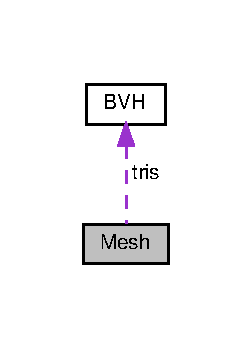
\includegraphics[width=121pt]{classMesh__coll__graph}
\end{center}
\end{figure}
\subsection*{Public Member Functions}
\begin{DoxyCompactItemize}
\item 
\mbox{\Hypertarget{classMesh_a5ac1070bda575410a98aa27a4f5e2951}\label{classMesh_a5ac1070bda575410a98aa27a4f5e2951}} 
{\bfseries Mesh} (vector$<$ \hyperlink{classTriangle}{Triangle} $\ast$$>$ tris)
\item 
\mbox{\Hypertarget{classMesh_a6ebe1c89c8b8c1ce48236547f48b014b}\label{classMesh_a6ebe1c89c8b8c1ce48236547f48b014b}} 
float {\bfseries get\+Height} (float x, float y)
\end{DoxyCompactItemize}
\subsection*{Public Attributes}
\begin{DoxyCompactItemize}
\item 
\mbox{\Hypertarget{classMesh_a8dbb906940e92cf062b9db91adeaa9ec}\label{classMesh_a8dbb906940e92cf062b9db91adeaa9ec}} 
\hyperlink{classBVH}{B\+VH} $\ast$ {\bfseries tris}
\end{DoxyCompactItemize}


The documentation for this class was generated from the following files\+:\begin{DoxyCompactItemize}
\item 
/home/behnam/\+C\+U\+D\+A-\/\+U\+R\+B/src/Mesh.\+h\item 
/home/behnam/\+C\+U\+D\+A-\/\+U\+R\+B/src/Mesh.\+cpp\end{DoxyCompactItemize}

\hypertarget{classMetParams}{}\section{Met\+Params Class Reference}
\label{classMetParams}\index{Met\+Params@{Met\+Params}}


Inheritance diagram for Met\+Params\+:
\nopagebreak
\begin{figure}[H]
\begin{center}
\leavevmode
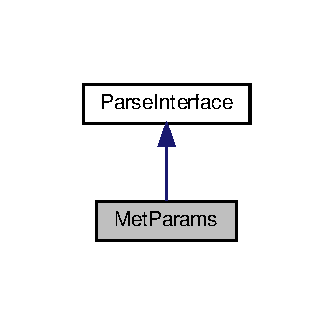
\includegraphics[width=160pt]{classMetParams__inherit__graph}
\end{center}
\end{figure}


Collaboration diagram for Met\+Params\+:
\nopagebreak
\begin{figure}[H]
\begin{center}
\leavevmode
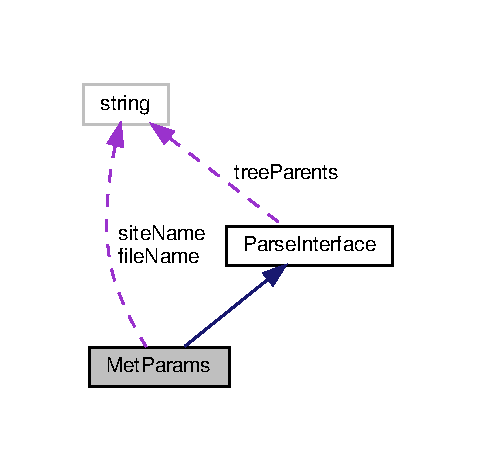
\includegraphics[width=229pt]{classMetParams__coll__graph}
\end{center}
\end{figure}
\subsection*{Public Member Functions}
\begin{DoxyCompactItemize}
\item 
virtual void \hyperlink{classMetParams_ad40706e0668d5e0248f39cc3a480b0af}{parse\+Values} ()
\end{DoxyCompactItemize}
\subsection*{Public Attributes}
\begin{DoxyCompactItemize}
\item 
\mbox{\Hypertarget{classMetParams_ac7cbbccae2ef3afa5cdf8c368cca0120}\label{classMetParams_ac7cbbccae2ef3afa5cdf8c368cca0120}} 
bool {\bfseries met\+Input\+Flag}
\item 
\mbox{\Hypertarget{classMetParams_a3ee150e743c92d214a1cdc73a8ca0d86}\label{classMetParams_a3ee150e743c92d214a1cdc73a8ca0d86}} 
int {\bfseries num\+\_\+sites}
\item 
\mbox{\Hypertarget{classMetParams_a2837878c4b2d008ceae2ed5238c2c897}\label{classMetParams_a2837878c4b2d008ceae2ed5238c2c897}} 
int {\bfseries max\+Size\+Data\+Points}
\item 
\mbox{\Hypertarget{classMetParams_a784eeb51250d096b7a3aa3d103ea1539}\label{classMetParams_a784eeb51250d096b7a3aa3d103ea1539}} 
std\+::string {\bfseries site\+Name}
\item 
\mbox{\Hypertarget{classMetParams_ad78ae52fa2be55f705527c308ad1712a}\label{classMetParams_ad78ae52fa2be55f705527c308ad1712a}} 
std\+::string {\bfseries file\+Name}
\item 
\mbox{\Hypertarget{classMetParams_a041964b4d55dc900b92220ff503aaa54}\label{classMetParams_a041964b4d55dc900b92220ff503aaa54}} 
std\+::vector$<$ \hyperlink{classSensor}{Sensor} $\ast$ $>$ {\bfseries sensors}
\end{DoxyCompactItemize}
\subsection*{Additional Inherited Members}


\subsection{Member Function Documentation}
\mbox{\Hypertarget{classMetParams_ad40706e0668d5e0248f39cc3a480b0af}\label{classMetParams_ad40706e0668d5e0248f39cc3a480b0af}} 
\index{Met\+Params@{Met\+Params}!parse\+Values@{parse\+Values}}
\index{parse\+Values@{parse\+Values}!Met\+Params@{Met\+Params}}
\subsubsection{\texorpdfstring{parse\+Values()}{parseValues()}}
{\footnotesize\ttfamily virtual void Met\+Params\+::parse\+Values (\begin{DoxyParamCaption}{ }\end{DoxyParamCaption})\hspace{0.3cm}{\ttfamily [inline]}, {\ttfamily [virtual]}}

Virtual function This is where we select what values we want to parse out of the xml file by calling the parseX functions above. 

Implements \hyperlink{classParseInterface_afca32108192ba0997c9e5a78189b0cbc}{Parse\+Interface}.



The documentation for this class was generated from the following file\+:\begin{DoxyCompactItemize}
\item 
/home/behnam/\+C\+U\+D\+A-\/\+U\+R\+B/src/Met\+Params.\+h\end{DoxyCompactItemize}

\hypertarget{classMyCommandLineArgs}{}\section{My\+Command\+Line\+Args Class Reference}
\label{classMyCommandLineArgs}\index{My\+Command\+Line\+Args@{My\+Command\+Line\+Args}}


Inheritance diagram for My\+Command\+Line\+Args\+:
\nopagebreak
\begin{figure}[H]
\begin{center}
\leavevmode
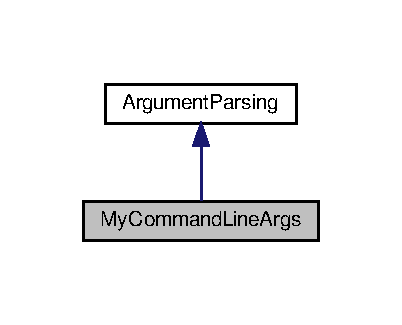
\includegraphics[width=193pt]{classMyCommandLineArgs__inherit__graph}
\end{center}
\end{figure}


Collaboration diagram for My\+Command\+Line\+Args\+:
\nopagebreak
\begin{figure}[H]
\begin{center}
\leavevmode
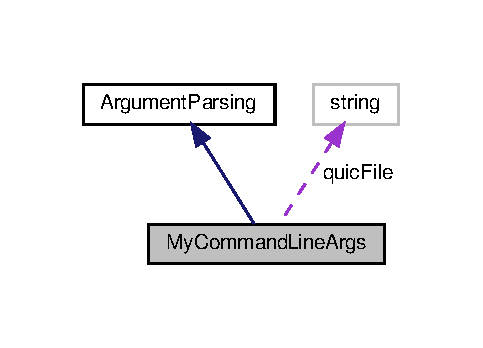
\includegraphics[width=232pt]{classMyCommandLineArgs__coll__graph}
\end{center}
\end{figure}
\subsection*{Public Member Functions}
\begin{DoxyCompactItemize}
\item 
\mbox{\Hypertarget{classMyCommandLineArgs_a4319e9c42c614a8c23f48252a8a35bd4}\label{classMyCommandLineArgs_a4319e9c42c614a8c23f48252a8a35bd4}} 
void {\bfseries process\+Arguments} (int argc, char $\ast$argv\mbox{[}$\,$\mbox{]})
\end{DoxyCompactItemize}
\subsection*{Public Attributes}
\begin{DoxyCompactItemize}
\item 
\mbox{\Hypertarget{classMyCommandLineArgs_a2da5f7a2c7df4f7805f8936ebee2a9b3}\label{classMyCommandLineArgs_a2da5f7a2c7df4f7805f8936ebee2a9b3}} 
bool {\bfseries verbose}
\item 
\mbox{\Hypertarget{classMyCommandLineArgs_afa9d9a970c7abd1275b9387719b0bccf}\label{classMyCommandLineArgs_afa9d9a970c7abd1275b9387719b0bccf}} 
std\+::string {\bfseries quic\+File}
\end{DoxyCompactItemize}
\subsection*{Additional Inherited Members}


The documentation for this class was generated from the following file\+:\begin{DoxyCompactItemize}
\item 
/home/behnam/\+C\+U\+D\+A-\/\+U\+R\+B/test/argparser.\+cpp\end{DoxyCompactItemize}

\hypertarget{classNetCDFData}{}\section{Net\+C\+D\+F\+Data Class Reference}
\label{classNetCDFData}\index{Net\+C\+D\+F\+Data@{Net\+C\+D\+F\+Data}}
\subsection*{Public Member Functions}
\begin{DoxyCompactItemize}
\item 
\mbox{\Hypertarget{classNetCDFData_a83a87e21aaf7a6b8832f703cb2428397}\label{classNetCDFData_a83a87e21aaf7a6b8832f703cb2428397}} 
void {\bfseries get\+Data} (float $\ast$newX, float $\ast$newY, float $\ast$newZ, std\+::vector$<$ double $>$ newU, std\+::vector$<$ double $>$ newV, std\+::vector$<$ double $>$ newW, int new\+DX, int new\+DY, int new\+DZ)
\item 
\mbox{\Hypertarget{classNetCDFData_a529a0cd09c197f3315fb2b13ac37c093}\label{classNetCDFData_a529a0cd09c197f3315fb2b13ac37c093}} 
void {\bfseries get\+Data\+I\+Cell} (int $\ast$new\+I\+Cell\+Flags, float $\ast$newX, float $\ast$newY, float $\ast$newZ, int n\+DX, int n\+DY, int n\+DZ, long new\+Size)
\item 
\mbox{\Hypertarget{classNetCDFData_a42691a22e2c7b0f1e229b5c2c778de79}\label{classNetCDFData_a42691a22e2c7b0f1e229b5c2c778de79}} 
void {\bfseries get\+Cut\+Cell\+Flags} (\hyperlink{classCell}{Cell} $\ast$cells)
\item 
\mbox{\Hypertarget{classNetCDFData_aa5dd60d0acf7db3857a9fda54d6245d6}\label{classNetCDFData_aa5dd60d0acf7db3857a9fda54d6245d6}} 
bool {\bfseries output\+I\+Cell\+Flags} (std\+::string file\+Name)
\item 
\mbox{\Hypertarget{classNetCDFData_ac883d61608e3d51a6ec9f2e10e061e13}\label{classNetCDFData_ac883d61608e3d51a6ec9f2e10e061e13}} 
bool {\bfseries output\+Cut\+Cell\+Flags} (std\+::string file\+Name)
\item 
\mbox{\Hypertarget{classNetCDFData_a859f33b4e381915183651dfb4eef4975}\label{classNetCDFData_a859f33b4e381915183651dfb4eef4975}} 
bool {\bfseries output\+Cell\+Face\+Results} (std\+::string file\+Name)
\end{DoxyCompactItemize}


The documentation for this class was generated from the following files\+:\begin{DoxyCompactItemize}
\item 
/home/behnam/\+C\+U\+D\+A-\/\+U\+R\+B/src/Net\+C\+D\+F\+Data.\+h\item 
/home/behnam/\+C\+U\+D\+A-\/\+U\+R\+B/src/Net\+C\+D\+F\+Data.\+cpp\end{DoxyCompactItemize}

\hypertarget{classNonPolyBuilding}{}\section{Non\+Poly\+Building Class Reference}
\label{classNonPolyBuilding}\index{Non\+Poly\+Building@{Non\+Poly\+Building}}


Inheritance diagram for Non\+Poly\+Building\+:
\nopagebreak
\begin{figure}[H]
\begin{center}
\leavevmode
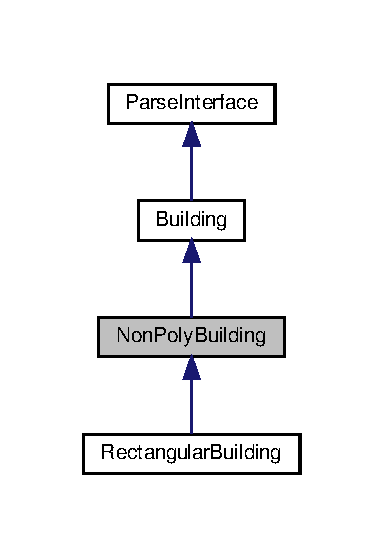
\includegraphics[width=184pt]{classNonPolyBuilding__inherit__graph}
\end{center}
\end{figure}


Collaboration diagram for Non\+Poly\+Building\+:
\nopagebreak
\begin{figure}[H]
\begin{center}
\leavevmode
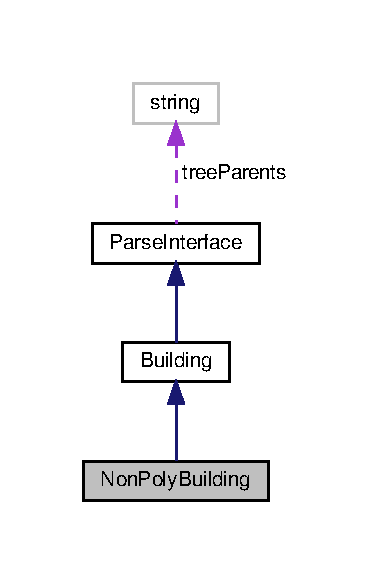
\includegraphics[width=179pt]{classNonPolyBuilding__coll__graph}
\end{center}
\end{figure}
\subsection*{Public Member Functions}
\begin{DoxyCompactItemize}
\item 
virtual void \hyperlink{classNonPolyBuilding_ace133756e0233d75b434fec5273b4414}{parse\+Values} ()=0
\end{DoxyCompactItemize}
\subsection*{Public Attributes}
\begin{DoxyCompactItemize}
\item 
\mbox{\Hypertarget{classNonPolyBuilding_a8336ab0b519db15cc53564ab1f4f17d4}\label{classNonPolyBuilding_a8336ab0b519db15cc53564ab1f4f17d4}} 
float {\bfseries x\+\_\+start}
\item 
\mbox{\Hypertarget{classNonPolyBuilding_a49a1c9d392aab2fb3168a31adc3633f1}\label{classNonPolyBuilding_a49a1c9d392aab2fb3168a31adc3633f1}} 
float {\bfseries y\+\_\+start}
\item 
\mbox{\Hypertarget{classNonPolyBuilding_a38a5d61b85eecc81389a401e7bd5377f}\label{classNonPolyBuilding_a38a5d61b85eecc81389a401e7bd5377f}} 
float {\bfseries L}
\item 
\mbox{\Hypertarget{classNonPolyBuilding_ab66753a47f7298de752f42d7ea84f393}\label{classNonPolyBuilding_ab66753a47f7298de752f42d7ea84f393}} 
float {\bfseries W}
\item 
\mbox{\Hypertarget{classNonPolyBuilding_a96c7173898b586ec5e624999ffb967cd}\label{classNonPolyBuilding_a96c7173898b586ec5e624999ffb967cd}} 
int {\bfseries i\+\_\+start}
\item 
\mbox{\Hypertarget{classNonPolyBuilding_ab0c41ec9b31a43dbad67f12b5bae530d}\label{classNonPolyBuilding_ab0c41ec9b31a43dbad67f12b5bae530d}} 
int {\bfseries i\+\_\+end}
\item 
\mbox{\Hypertarget{classNonPolyBuilding_a0320d925ddd784f039265c5726802213}\label{classNonPolyBuilding_a0320d925ddd784f039265c5726802213}} 
int {\bfseries j\+\_\+start}
\item 
\mbox{\Hypertarget{classNonPolyBuilding_a989c0757ee74e749dedaf17a8b5f4375}\label{classNonPolyBuilding_a989c0757ee74e749dedaf17a8b5f4375}} 
int {\bfseries j\+\_\+end}
\item 
\mbox{\Hypertarget{classNonPolyBuilding_ac09986f076f8285e3307b8dd07202d48}\label{classNonPolyBuilding_ac09986f076f8285e3307b8dd07202d48}} 
int {\bfseries k\+\_\+end}
\item 
\mbox{\Hypertarget{classNonPolyBuilding_a63d89a349607e6c72eeff359ca869921}\label{classNonPolyBuilding_a63d89a349607e6c72eeff359ca869921}} 
int {\bfseries i\+\_\+cut\+\_\+start}
\item 
\mbox{\Hypertarget{classNonPolyBuilding_abf875cb22fdd4bba2a673845e1d7f320}\label{classNonPolyBuilding_abf875cb22fdd4bba2a673845e1d7f320}} 
int {\bfseries i\+\_\+cut\+\_\+end}
\item 
\mbox{\Hypertarget{classNonPolyBuilding_a7258b062bc3d755772d5cda15a2bb3ed}\label{classNonPolyBuilding_a7258b062bc3d755772d5cda15a2bb3ed}} 
int {\bfseries j\+\_\+cut\+\_\+start}
\item 
\mbox{\Hypertarget{classNonPolyBuilding_ab49ed1020318238c329b71c970e2fdc7}\label{classNonPolyBuilding_ab49ed1020318238c329b71c970e2fdc7}} 
int {\bfseries j\+\_\+cut\+\_\+end}
\item 
\mbox{\Hypertarget{classNonPolyBuilding_ac8cd541903d56d398c6df5d279c00d99}\label{classNonPolyBuilding_ac8cd541903d56d398c6df5d279c00d99}} 
int {\bfseries k\+\_\+cut\+\_\+end}
\item 
\mbox{\Hypertarget{classNonPolyBuilding_a7bdddbe9ef9948491e0560310e4afd60}\label{classNonPolyBuilding_a7bdddbe9ef9948491e0560310e4afd60}} 
float {\bfseries H}
\end{DoxyCompactItemize}
\subsection*{Additional Inherited Members}


\subsection{Member Function Documentation}
\mbox{\Hypertarget{classNonPolyBuilding_ace133756e0233d75b434fec5273b4414}\label{classNonPolyBuilding_ace133756e0233d75b434fec5273b4414}} 
\index{Non\+Poly\+Building@{Non\+Poly\+Building}!parse\+Values@{parse\+Values}}
\index{parse\+Values@{parse\+Values}!Non\+Poly\+Building@{Non\+Poly\+Building}}
\subsubsection{\texorpdfstring{parse\+Values()}{parseValues()}}
{\footnotesize\ttfamily virtual void Non\+Poly\+Building\+::parse\+Values (\begin{DoxyParamCaption}{ }\end{DoxyParamCaption})\hspace{0.3cm}{\ttfamily [pure virtual]}}

Virtual function This is where we select what values we want to parse out of the xml file by calling the parseX functions above. 

Implements \hyperlink{classBuilding_a7782e7933a009fcfee4d186e62d34b43}{Building}.



Implemented in \hyperlink{classRectangularBuilding_adbc6b832c817fc06f9bc2e51561a7e81}{Rectangular\+Building}.



The documentation for this class was generated from the following file\+:\begin{DoxyCompactItemize}
\item 
/home/behnam/\+C\+U\+D\+A-\/\+U\+R\+B/src/Non\+Poly\+Building.\+h\end{DoxyCompactItemize}

\hypertarget{classP}{}\section{P Class Reference}
\label{classP}\index{P@{P}}


Inheritance diagram for P\+:
\nopagebreak
\begin{figure}[H]
\begin{center}
\leavevmode
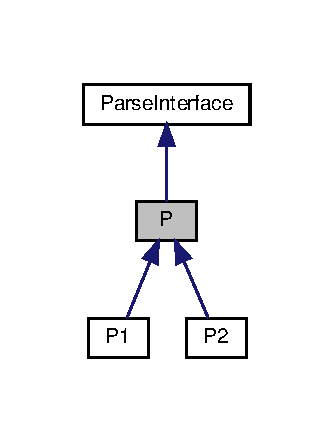
\includegraphics[width=160pt]{classP__inherit__graph}
\end{center}
\end{figure}


Collaboration diagram for P\+:
\nopagebreak
\begin{figure}[H]
\begin{center}
\leavevmode
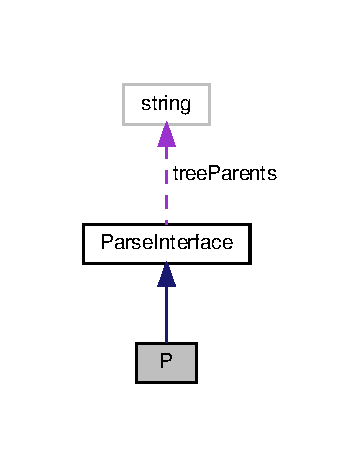
\includegraphics[width=174pt]{classP__coll__graph}
\end{center}
\end{figure}
\subsection*{Public Member Functions}
\begin{DoxyCompactItemize}
\item 
\mbox{\Hypertarget{classP_ad4c6552ef6e0bca9f4217af419abf12b}\label{classP_ad4c6552ef6e0bca9f4217af419abf12b}} 
virtual void {\bfseries output} ()=0
\end{DoxyCompactItemize}
\subsection*{Additional Inherited Members}


The documentation for this class was generated from the following file\+:\begin{DoxyCompactItemize}
\item 
/home/behnam/\+C\+U\+D\+A-\/\+U\+R\+B/xml\+Testing/P.\+h\end{DoxyCompactItemize}

\hypertarget{classP1}{}\section{P1 Class Reference}
\label{classP1}\index{P1@{P1}}


Inheritance diagram for P1\+:
\nopagebreak
\begin{figure}[H]
\begin{center}
\leavevmode
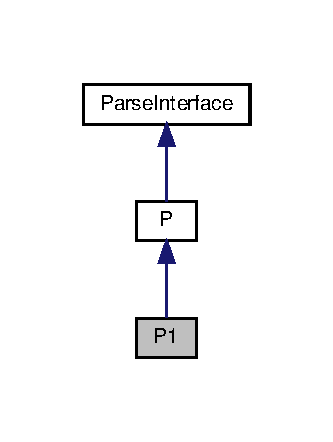
\includegraphics[width=160pt]{classP1__inherit__graph}
\end{center}
\end{figure}


Collaboration diagram for P1\+:
\nopagebreak
\begin{figure}[H]
\begin{center}
\leavevmode
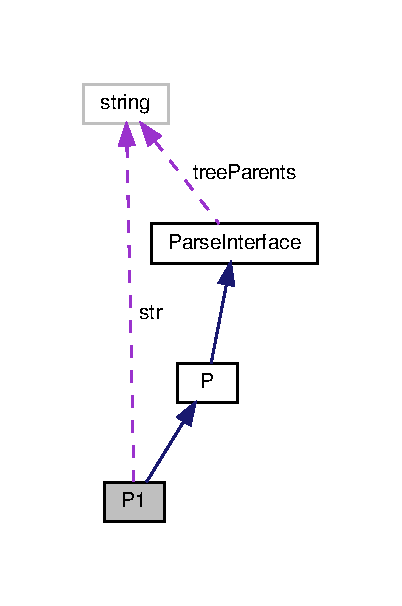
\includegraphics[width=193pt]{classP1__coll__graph}
\end{center}
\end{figure}
\subsection*{Public Member Functions}
\begin{DoxyCompactItemize}
\item 
void \hyperlink{classP1_aea4d99ff4e45862292d2dbb83ec32363}{parse\+Values} ()
\item 
\mbox{\Hypertarget{classP1_a49ad189d8949a0bca3097947830cd984}\label{classP1_a49ad189d8949a0bca3097947830cd984}} 
virtual void {\bfseries output} ()
\end{DoxyCompactItemize}
\subsection*{Public Attributes}
\begin{DoxyCompactItemize}
\item 
\mbox{\Hypertarget{classP1_a45b090af4331715d98a38a1a2cb4ba05}\label{classP1_a45b090af4331715d98a38a1a2cb4ba05}} 
std\+::string {\bfseries str}
\item 
\mbox{\Hypertarget{classP1_ab9a666a647699c37220d47c275e2474e}\label{classP1_ab9a666a647699c37220d47c275e2474e}} 
int {\bfseries x}
\end{DoxyCompactItemize}
\subsection*{Additional Inherited Members}


\subsection{Member Function Documentation}
\mbox{\Hypertarget{classP1_aea4d99ff4e45862292d2dbb83ec32363}\label{classP1_aea4d99ff4e45862292d2dbb83ec32363}} 
\index{P1@{P1}!parse\+Values@{parse\+Values}}
\index{parse\+Values@{parse\+Values}!P1@{P1}}
\subsubsection{\texorpdfstring{parse\+Values()}{parseValues()}}
{\footnotesize\ttfamily void P1\+::parse\+Values (\begin{DoxyParamCaption}{ }\end{DoxyParamCaption})\hspace{0.3cm}{\ttfamily [inline]}, {\ttfamily [virtual]}}

Virtual function This is where we select what values we want to parse out of the xml file by calling the parseX functions above. 

Implements \hyperlink{classParseInterface_afca32108192ba0997c9e5a78189b0cbc}{Parse\+Interface}.



The documentation for this class was generated from the following file\+:\begin{DoxyCompactItemize}
\item 
/home/behnam/\+C\+U\+D\+A-\/\+U\+R\+B/xml\+Testing/P.\+h\end{DoxyCompactItemize}

\hypertarget{classP2}{}\section{P2 Class Reference}
\label{classP2}\index{P2@{P2}}


Inheritance diagram for P2\+:
\nopagebreak
\begin{figure}[H]
\begin{center}
\leavevmode
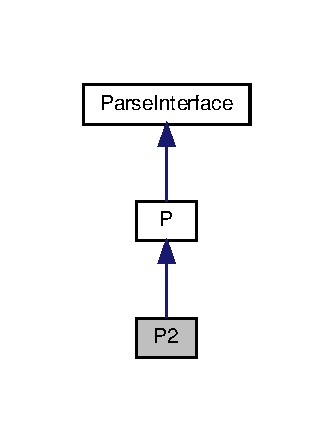
\includegraphics[width=160pt]{classP2__inherit__graph}
\end{center}
\end{figure}


Collaboration diagram for P2\+:
\nopagebreak
\begin{figure}[H]
\begin{center}
\leavevmode
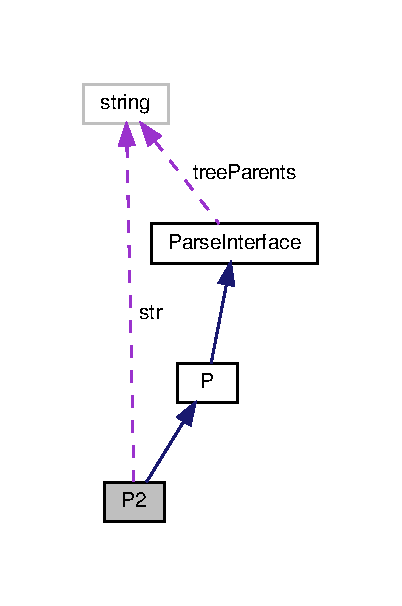
\includegraphics[width=193pt]{classP2__coll__graph}
\end{center}
\end{figure}
\subsection*{Public Member Functions}
\begin{DoxyCompactItemize}
\item 
void \hyperlink{classP2_a3b8928a6e7dda94f06dab603420cd8c7}{parse\+Values} ()
\item 
\mbox{\Hypertarget{classP2_a01f565d79b5c794b945ea2d9ecd92dbd}\label{classP2_a01f565d79b5c794b945ea2d9ecd92dbd}} 
virtual void {\bfseries output} ()
\end{DoxyCompactItemize}
\subsection*{Public Attributes}
\begin{DoxyCompactItemize}
\item 
\mbox{\Hypertarget{classP2_ade6643522e8b3766a24c0e873283e5e0}\label{classP2_ade6643522e8b3766a24c0e873283e5e0}} 
std\+::string {\bfseries str}
\item 
\mbox{\Hypertarget{classP2_ada44448410a02423bfa909a90dfa9165}\label{classP2_ada44448410a02423bfa909a90dfa9165}} 
char {\bfseries c}
\item 
\mbox{\Hypertarget{classP2_acb53c80d81cd6e329182fc7ed051e4f7}\label{classP2_acb53c80d81cd6e329182fc7ed051e4f7}} 
float {\bfseries f}
\item 
\mbox{\Hypertarget{classP2_a29fe0aa9eaac637d3647f440a7cbb823}\label{classP2_a29fe0aa9eaac637d3647f440a7cbb823}} 
float {\bfseries q}
\end{DoxyCompactItemize}
\subsection*{Additional Inherited Members}


\subsection{Member Function Documentation}
\mbox{\Hypertarget{classP2_a3b8928a6e7dda94f06dab603420cd8c7}\label{classP2_a3b8928a6e7dda94f06dab603420cd8c7}} 
\index{P2@{P2}!parse\+Values@{parse\+Values}}
\index{parse\+Values@{parse\+Values}!P2@{P2}}
\subsubsection{\texorpdfstring{parse\+Values()}{parseValues()}}
{\footnotesize\ttfamily void P2\+::parse\+Values (\begin{DoxyParamCaption}{ }\end{DoxyParamCaption})\hspace{0.3cm}{\ttfamily [inline]}, {\ttfamily [virtual]}}

Virtual function This is where we select what values we want to parse out of the xml file by calling the parseX functions above. 

Implements \hyperlink{classParseInterface_afca32108192ba0997c9e5a78189b0cbc}{Parse\+Interface}.



The documentation for this class was generated from the following file\+:\begin{DoxyCompactItemize}
\item 
/home/behnam/\+C\+U\+D\+A-\/\+U\+R\+B/xml\+Testing/P.\+h\end{DoxyCompactItemize}

\hypertarget{classParseException}{}\section{Parse\+Exception Class Reference}
\label{classParseException}\index{Parse\+Exception@{Parse\+Exception}}


{\ttfamily \#include $<$Parse\+Exception.\+h$>$}



Inheritance diagram for Parse\+Exception\+:
\nopagebreak
\begin{figure}[H]
\begin{center}
\leavevmode
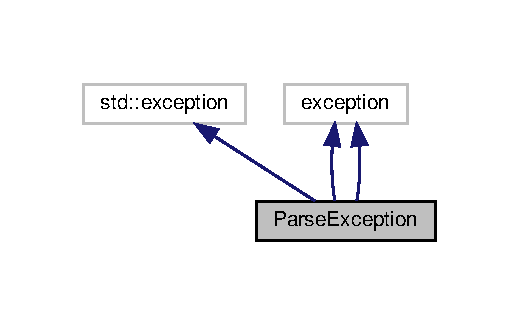
\includegraphics[width=249pt]{classParseException__inherit__graph}
\end{center}
\end{figure}


Collaboration diagram for Parse\+Exception\+:
\nopagebreak
\begin{figure}[H]
\begin{center}
\leavevmode
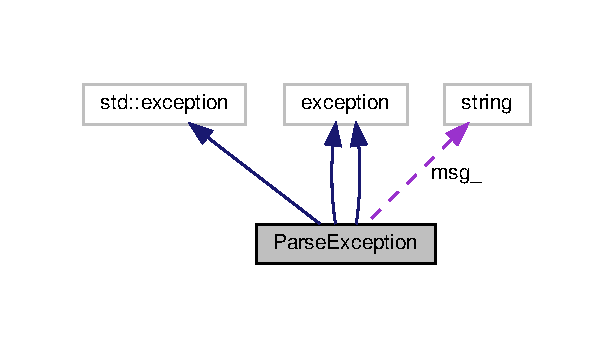
\includegraphics[width=295pt]{classParseException__coll__graph}
\end{center}
\end{figure}
\subsection*{Public Member Functions}
\begin{DoxyCompactItemize}
\item 
\hyperlink{classParseException_a0e2db737183a1801d528102617ddc3c4}{Parse\+Exception} (const char $\ast$message)
\item 
\hyperlink{classParseException_a162b338172e869ef6e308b4489abf95b}{Parse\+Exception} (const std\+::string \&message)
\item 
virtual \hyperlink{classParseException_a59f11745728ad1ede341f2dda48e79b6}{$\sim$\+Parse\+Exception} ()  throw ()
\item 
virtual const char $\ast$ \hyperlink{classParseException_a7c96d5c467fe71354528570caf9209cd}{what} () const  throw ()
\item 
\hyperlink{classParseException_a0e2db737183a1801d528102617ddc3c4}{Parse\+Exception} (const char $\ast$message)
\item 
\hyperlink{classParseException_a162b338172e869ef6e308b4489abf95b}{Parse\+Exception} (const std\+::string \&message)
\item 
virtual \hyperlink{classParseException_a59f11745728ad1ede341f2dda48e79b6}{$\sim$\+Parse\+Exception} ()  throw ()
\item 
virtual const char $\ast$ \hyperlink{classParseException_a7c96d5c467fe71354528570caf9209cd}{what} () const  throw ()
\item 
\hyperlink{classParseException_a0e2db737183a1801d528102617ddc3c4}{Parse\+Exception} (const char $\ast$message)
\item 
\hyperlink{classParseException_a162b338172e869ef6e308b4489abf95b}{Parse\+Exception} (const std\+::string \&message)
\item 
virtual \hyperlink{classParseException_a59f11745728ad1ede341f2dda48e79b6}{$\sim$\+Parse\+Exception} ()  throw ()
\item 
virtual const char $\ast$ \hyperlink{classParseException_a7c96d5c467fe71354528570caf9209cd}{what} () const  throw ()
\end{DoxyCompactItemize}
\subsection*{Protected Attributes}
\begin{DoxyCompactItemize}
\item 
std\+::string \hyperlink{classParseException_a1e21a45e6538896bb5c71cc7390d986b}{msg\+\_\+}
\end{DoxyCompactItemize}


\subsection{Detailed Description}
This class is an extension of the standard exception class. The specifics of this exception arre to identify when a parameter is required to exist but is not present in the X\+ML. 

\subsection{Constructor \& Destructor Documentation}
\mbox{\Hypertarget{classParseException_a0e2db737183a1801d528102617ddc3c4}\label{classParseException_a0e2db737183a1801d528102617ddc3c4}} 
\index{Parse\+Exception@{Parse\+Exception}!Parse\+Exception@{Parse\+Exception}}
\index{Parse\+Exception@{Parse\+Exception}!Parse\+Exception@{Parse\+Exception}}
\subsubsection{\texorpdfstring{Parse\+Exception()}{ParseException()}\hspace{0.1cm}{\footnotesize\ttfamily [1/6]}}
{\footnotesize\ttfamily Parse\+Exception\+::\+Parse\+Exception (\begin{DoxyParamCaption}\item[{const char $\ast$}]{message }\end{DoxyParamCaption})\hspace{0.3cm}{\ttfamily [inline]}, {\ttfamily [explicit]}}

Constructor (\hyperlink{classC}{C} strings). 
\begin{DoxyParams}{Parameters}
{\em message} & C-\/style string error message. The string contents are copied upon construction. Hence, responsibility for deleting the char$\ast$ lies with the caller. \\
\hline
\end{DoxyParams}
\mbox{\Hypertarget{classParseException_a162b338172e869ef6e308b4489abf95b}\label{classParseException_a162b338172e869ef6e308b4489abf95b}} 
\index{Parse\+Exception@{Parse\+Exception}!Parse\+Exception@{Parse\+Exception}}
\index{Parse\+Exception@{Parse\+Exception}!Parse\+Exception@{Parse\+Exception}}
\subsubsection{\texorpdfstring{Parse\+Exception()}{ParseException()}\hspace{0.1cm}{\footnotesize\ttfamily [2/6]}}
{\footnotesize\ttfamily Parse\+Exception\+::\+Parse\+Exception (\begin{DoxyParamCaption}\item[{const std\+::string \&}]{message }\end{DoxyParamCaption})\hspace{0.3cm}{\ttfamily [inline]}, {\ttfamily [explicit]}}

Constructor (C++ S\+TL strings). 
\begin{DoxyParams}{Parameters}
{\em message} & The error message. \\
\hline
\end{DoxyParams}
\mbox{\Hypertarget{classParseException_a59f11745728ad1ede341f2dda48e79b6}\label{classParseException_a59f11745728ad1ede341f2dda48e79b6}} 
\index{Parse\+Exception@{Parse\+Exception}!````~Parse\+Exception@{$\sim$\+Parse\+Exception}}
\index{````~Parse\+Exception@{$\sim$\+Parse\+Exception}!Parse\+Exception@{Parse\+Exception}}
\subsubsection{\texorpdfstring{$\sim$\+Parse\+Exception()}{~ParseException()}\hspace{0.1cm}{\footnotesize\ttfamily [1/3]}}
{\footnotesize\ttfamily virtual Parse\+Exception\+::$\sim$\+Parse\+Exception (\begin{DoxyParamCaption}{ }\end{DoxyParamCaption}) throw  ) \hspace{0.3cm}{\ttfamily [inline]}, {\ttfamily [virtual]}}

Destructor. Virtual to allow for subclassing. \mbox{\Hypertarget{classParseException_a0e2db737183a1801d528102617ddc3c4}\label{classParseException_a0e2db737183a1801d528102617ddc3c4}} 
\index{Parse\+Exception@{Parse\+Exception}!Parse\+Exception@{Parse\+Exception}}
\index{Parse\+Exception@{Parse\+Exception}!Parse\+Exception@{Parse\+Exception}}
\subsubsection{\texorpdfstring{Parse\+Exception()}{ParseException()}\hspace{0.1cm}{\footnotesize\ttfamily [3/6]}}
{\footnotesize\ttfamily Parse\+Exception\+::\+Parse\+Exception (\begin{DoxyParamCaption}\item[{const char $\ast$}]{message }\end{DoxyParamCaption})\hspace{0.3cm}{\ttfamily [inline]}, {\ttfamily [explicit]}}

Constructor (\hyperlink{classC}{C} strings). 
\begin{DoxyParams}{Parameters}
{\em message} & C-\/style string error message. The string contents are copied upon construction. Hence, responsibility for deleting the char$\ast$ lies with the caller. \\
\hline
\end{DoxyParams}
\mbox{\Hypertarget{classParseException_a162b338172e869ef6e308b4489abf95b}\label{classParseException_a162b338172e869ef6e308b4489abf95b}} 
\index{Parse\+Exception@{Parse\+Exception}!Parse\+Exception@{Parse\+Exception}}
\index{Parse\+Exception@{Parse\+Exception}!Parse\+Exception@{Parse\+Exception}}
\subsubsection{\texorpdfstring{Parse\+Exception()}{ParseException()}\hspace{0.1cm}{\footnotesize\ttfamily [4/6]}}
{\footnotesize\ttfamily Parse\+Exception\+::\+Parse\+Exception (\begin{DoxyParamCaption}\item[{const std\+::string \&}]{message }\end{DoxyParamCaption})\hspace{0.3cm}{\ttfamily [inline]}, {\ttfamily [explicit]}}

Constructor (C++ S\+TL strings). 
\begin{DoxyParams}{Parameters}
{\em message} & The error message. \\
\hline
\end{DoxyParams}
\mbox{\Hypertarget{classParseException_a59f11745728ad1ede341f2dda48e79b6}\label{classParseException_a59f11745728ad1ede341f2dda48e79b6}} 
\index{Parse\+Exception@{Parse\+Exception}!````~Parse\+Exception@{$\sim$\+Parse\+Exception}}
\index{````~Parse\+Exception@{$\sim$\+Parse\+Exception}!Parse\+Exception@{Parse\+Exception}}
\subsubsection{\texorpdfstring{$\sim$\+Parse\+Exception()}{~ParseException()}\hspace{0.1cm}{\footnotesize\ttfamily [2/3]}}
{\footnotesize\ttfamily virtual Parse\+Exception\+::$\sim$\+Parse\+Exception (\begin{DoxyParamCaption}{ }\end{DoxyParamCaption}) throw  ) \hspace{0.3cm}{\ttfamily [inline]}, {\ttfamily [virtual]}}

Destructor. Virtual to allow for subclassing. \mbox{\Hypertarget{classParseException_a0e2db737183a1801d528102617ddc3c4}\label{classParseException_a0e2db737183a1801d528102617ddc3c4}} 
\index{Parse\+Exception@{Parse\+Exception}!Parse\+Exception@{Parse\+Exception}}
\index{Parse\+Exception@{Parse\+Exception}!Parse\+Exception@{Parse\+Exception}}
\subsubsection{\texorpdfstring{Parse\+Exception()}{ParseException()}\hspace{0.1cm}{\footnotesize\ttfamily [5/6]}}
{\footnotesize\ttfamily Parse\+Exception\+::\+Parse\+Exception (\begin{DoxyParamCaption}\item[{const char $\ast$}]{message }\end{DoxyParamCaption})\hspace{0.3cm}{\ttfamily [inline]}, {\ttfamily [explicit]}}

Constructor (\hyperlink{classC}{C} strings). 
\begin{DoxyParams}{Parameters}
{\em message} & C-\/style string error message. The string contents are copied upon construction. Hence, responsibility for deleting the char$\ast$ lies with the caller. \\
\hline
\end{DoxyParams}
\mbox{\Hypertarget{classParseException_a162b338172e869ef6e308b4489abf95b}\label{classParseException_a162b338172e869ef6e308b4489abf95b}} 
\index{Parse\+Exception@{Parse\+Exception}!Parse\+Exception@{Parse\+Exception}}
\index{Parse\+Exception@{Parse\+Exception}!Parse\+Exception@{Parse\+Exception}}
\subsubsection{\texorpdfstring{Parse\+Exception()}{ParseException()}\hspace{0.1cm}{\footnotesize\ttfamily [6/6]}}
{\footnotesize\ttfamily Parse\+Exception\+::\+Parse\+Exception (\begin{DoxyParamCaption}\item[{const std\+::string \&}]{message }\end{DoxyParamCaption})\hspace{0.3cm}{\ttfamily [inline]}, {\ttfamily [explicit]}}

Constructor (C++ S\+TL strings). 
\begin{DoxyParams}{Parameters}
{\em message} & The error message. \\
\hline
\end{DoxyParams}
\mbox{\Hypertarget{classParseException_a59f11745728ad1ede341f2dda48e79b6}\label{classParseException_a59f11745728ad1ede341f2dda48e79b6}} 
\index{Parse\+Exception@{Parse\+Exception}!````~Parse\+Exception@{$\sim$\+Parse\+Exception}}
\index{````~Parse\+Exception@{$\sim$\+Parse\+Exception}!Parse\+Exception@{Parse\+Exception}}
\subsubsection{\texorpdfstring{$\sim$\+Parse\+Exception()}{~ParseException()}\hspace{0.1cm}{\footnotesize\ttfamily [3/3]}}
{\footnotesize\ttfamily virtual Parse\+Exception\+::$\sim$\+Parse\+Exception (\begin{DoxyParamCaption}{ }\end{DoxyParamCaption}) throw  ) \hspace{0.3cm}{\ttfamily [inline]}, {\ttfamily [virtual]}}

Destructor. Virtual to allow for subclassing. 

\subsection{Member Function Documentation}
\mbox{\Hypertarget{classParseException_a7c96d5c467fe71354528570caf9209cd}\label{classParseException_a7c96d5c467fe71354528570caf9209cd}} 
\index{Parse\+Exception@{Parse\+Exception}!what@{what}}
\index{what@{what}!Parse\+Exception@{Parse\+Exception}}
\subsubsection{\texorpdfstring{what()}{what()}\hspace{0.1cm}{\footnotesize\ttfamily [1/3]}}
{\footnotesize\ttfamily virtual const char$\ast$ Parse\+Exception\+::what (\begin{DoxyParamCaption}{ }\end{DoxyParamCaption}) const throw  ) \hspace{0.3cm}{\ttfamily [inline]}, {\ttfamily [virtual]}}

Returns a pointer to the (constant) error description. \begin{DoxyReturn}{Returns}
\hyperlink{classA}{A} pointer to a const char$\ast$. The underlying memory is in posession of the Exception object. Callers must not attempt to free the memory. 
\end{DoxyReturn}
\mbox{\Hypertarget{classParseException_a7c96d5c467fe71354528570caf9209cd}\label{classParseException_a7c96d5c467fe71354528570caf9209cd}} 
\index{Parse\+Exception@{Parse\+Exception}!what@{what}}
\index{what@{what}!Parse\+Exception@{Parse\+Exception}}
\subsubsection{\texorpdfstring{what()}{what()}\hspace{0.1cm}{\footnotesize\ttfamily [2/3]}}
{\footnotesize\ttfamily virtual const char$\ast$ Parse\+Exception\+::what (\begin{DoxyParamCaption}{ }\end{DoxyParamCaption}) const throw  ) \hspace{0.3cm}{\ttfamily [inline]}, {\ttfamily [virtual]}}

Returns a pointer to the (constant) error description. \begin{DoxyReturn}{Returns}
\hyperlink{classA}{A} pointer to a const char$\ast$. The underlying memory is in posession of the Exception object. Callers must not attempt to free the memory. 
\end{DoxyReturn}
\mbox{\Hypertarget{classParseException_a7c96d5c467fe71354528570caf9209cd}\label{classParseException_a7c96d5c467fe71354528570caf9209cd}} 
\index{Parse\+Exception@{Parse\+Exception}!what@{what}}
\index{what@{what}!Parse\+Exception@{Parse\+Exception}}
\subsubsection{\texorpdfstring{what()}{what()}\hspace{0.1cm}{\footnotesize\ttfamily [3/3]}}
{\footnotesize\ttfamily virtual const char$\ast$ Parse\+Exception\+::what (\begin{DoxyParamCaption}{ }\end{DoxyParamCaption}) const throw  ) \hspace{0.3cm}{\ttfamily [inline]}, {\ttfamily [virtual]}}

Returns a pointer to the (constant) error description. \begin{DoxyReturn}{Returns}
\hyperlink{classA}{A} pointer to a const char$\ast$. The underlying memory is in posession of the Exception object. Callers must not attempt to free the memory. 
\end{DoxyReturn}


\subsection{Member Data Documentation}
\mbox{\Hypertarget{classParseException_a1e21a45e6538896bb5c71cc7390d986b}\label{classParseException_a1e21a45e6538896bb5c71cc7390d986b}} 
\index{Parse\+Exception@{Parse\+Exception}!msg\+\_\+@{msg\+\_\+}}
\index{msg\+\_\+@{msg\+\_\+}!Parse\+Exception@{Parse\+Exception}}
\subsubsection{\texorpdfstring{msg\+\_\+}{msg\_}}
{\footnotesize\ttfamily std\+::string Parse\+Exception\+::msg\+\_\+\hspace{0.3cm}{\ttfamily [protected]}}

Error message. 

The documentation for this class was generated from the following file\+:\begin{DoxyCompactItemize}
\item 
/home/behnam/\+C\+U\+D\+A-\/\+U\+R\+B/src/util/Parse\+Exception.\+h\end{DoxyCompactItemize}

\hypertarget{classParseInterface}{}\section{Parse\+Interface Class Reference}
\label{classParseInterface}\index{Parse\+Interface@{Parse\+Interface}}


{\ttfamily \#include $<$Parse\+Interface.\+h$>$}



Inheritance diagram for Parse\+Interface\+:
\nopagebreak
\begin{figure}[H]
\begin{center}
\leavevmode
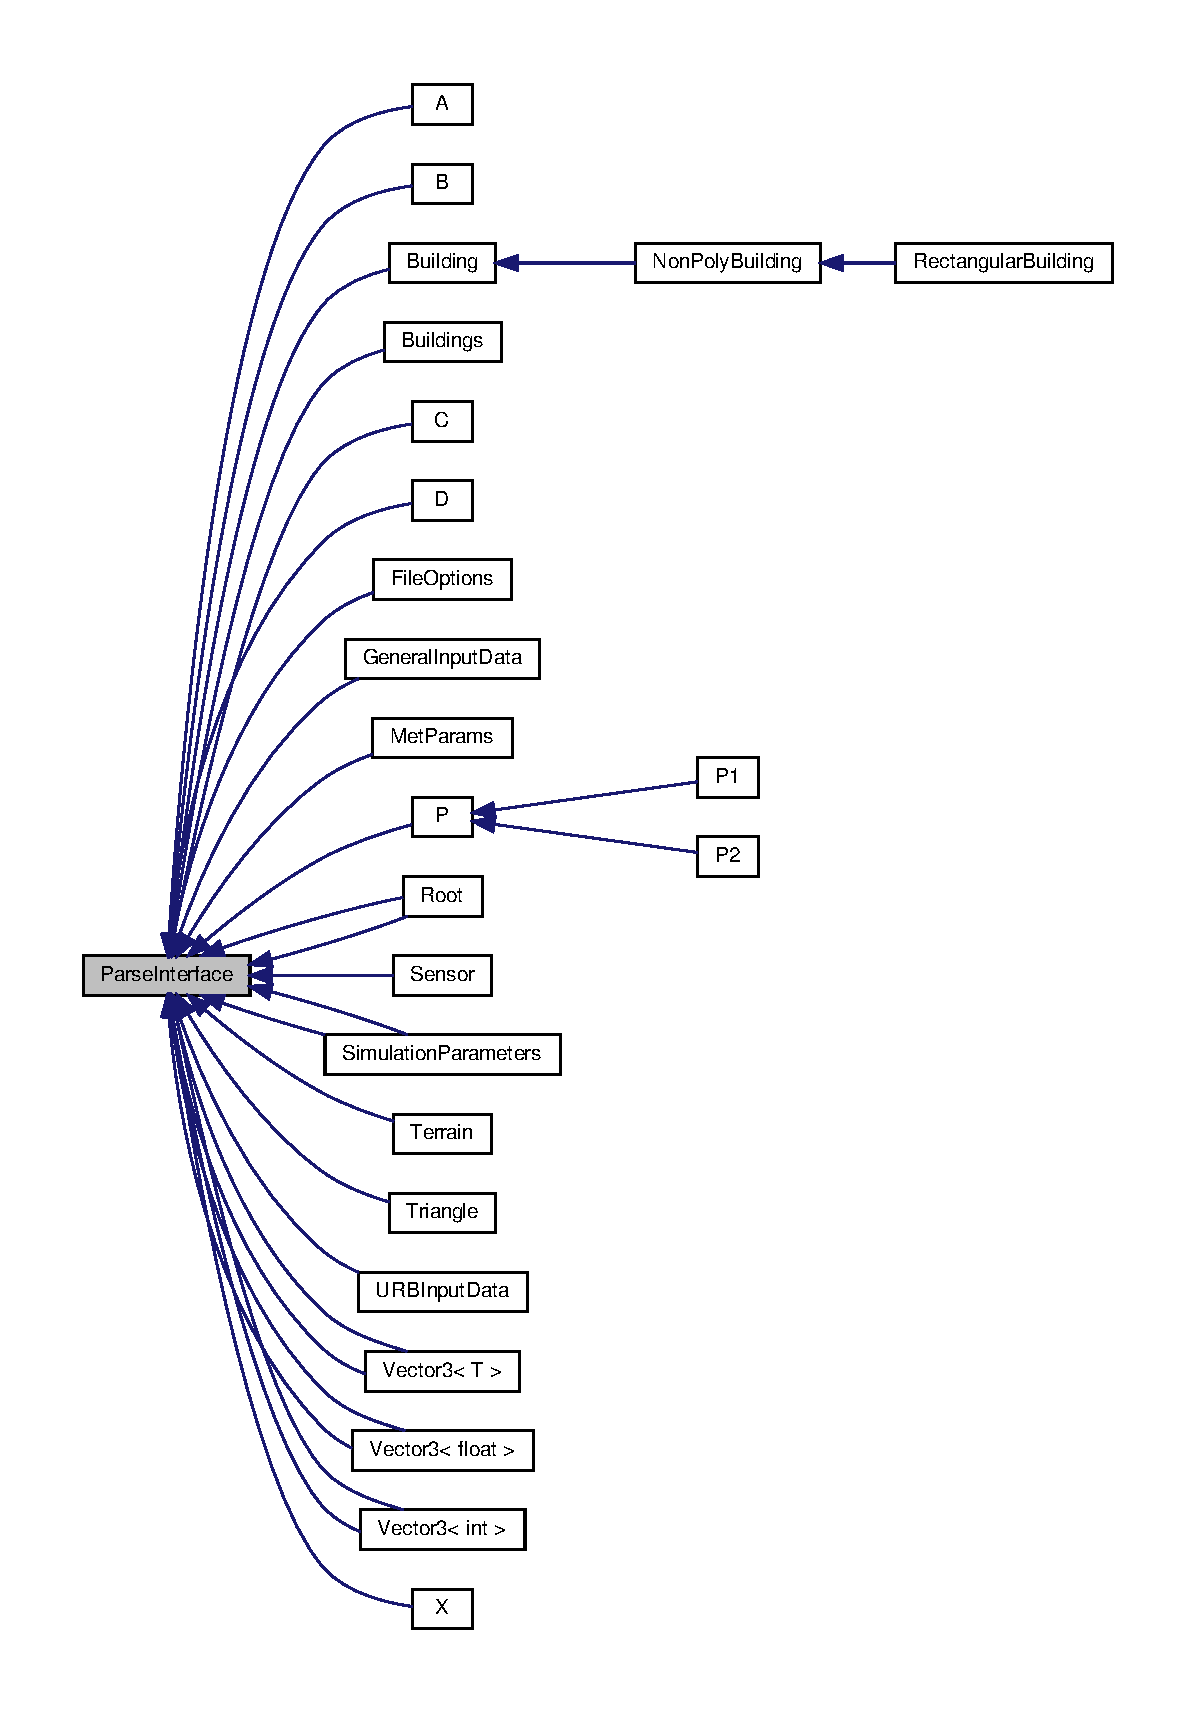
\includegraphics[width=350pt]{classParseInterface__inherit__graph}
\end{center}
\end{figure}


Collaboration diagram for Parse\+Interface\+:
\nopagebreak
\begin{figure}[H]
\begin{center}
\leavevmode
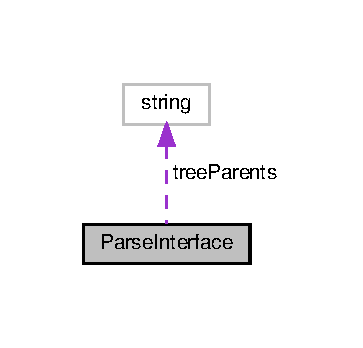
\includegraphics[width=174pt]{classParseInterface__coll__graph}
\end{center}
\end{figure}
\subsection*{Public Member Functions}
\begin{DoxyCompactItemize}
\item 
{\footnotesize template$<$typename T $>$ }\\void \hyperlink{classParseInterface_a86b7469a47ed83434a55ca1974a7287e}{parse\+Primitive} (bool is\+Req, T \&val, const std\+::string tag)
\item 
{\footnotesize template$<$typename T $>$ }\\void \hyperlink{classParseInterface_a0d16b9baf79eb34c63914159798dc1eb}{parse\+Multi\+Primitives} (bool is\+Req, std\+::vector$<$ T $>$ \&vals, const std\+::string tag)
\item 
{\footnotesize template$<$typename T $>$ }\\void \hyperlink{classParseInterface_a289c74beb3acea103f9864f2225bce00}{parse\+Element} (bool is\+Req, T $\ast$\&ele, const std\+::string tag)
\item 
{\footnotesize template$<$typename T $>$ }\\void \hyperlink{classParseInterface_aca9ff3a3139e6939cb7b0c8612d4a609}{parse\+Multi\+Elements} (bool is\+Req, std\+::vector$<$ T $\ast$$>$ \&eles, const std\+::string tag)
\item 
{\footnotesize template$<$typename T , typename X , typename... A\+R\+GS$>$ }\\void \hyperlink{classParseInterface_af24b31d7ffc3029b8a7a67f986ab414f}{parse\+Polymorph} (bool is\+Req, T $\ast$\&ele, \hyperlink{classX}{X} poly, A\+R\+G\+S... args)
\item 
{\footnotesize template$<$typename T , typename X $>$ }\\void \hyperlink{classParseInterface_a3eddda17bca991a068b171fb6949bce8}{parse\+Polymorph} (bool is\+Req, T $\ast$\&ele, \hyperlink{classX}{X} poly)
\item 
{\footnotesize template$<$typename T , typename X , typename... A\+R\+GS$>$ }\\void \hyperlink{classParseInterface_ab742098ba7badf016388bd10b32fb1ee}{parse\+Multi\+Polymorphs} (bool is\+Req, std\+::vector$<$ T $\ast$$>$ \&eles, \hyperlink{classX}{X} poly, A\+R\+G\+S... args)
\item 
{\footnotesize template$<$typename T , typename X $>$ }\\void \hyperlink{classParseInterface_a3d1afd8bdd00110808e3c42320556544}{parse\+Multi\+Polymorphs} (bool is\+Req, std\+::vector$<$ T $\ast$$>$ \&eles, \hyperlink{classX}{X} poly)
\item 
{\footnotesize template$<$typename T $>$ }\\void \hyperlink{classParseInterface_a60c8afbe5369965c8855491bb3f75668}{parse\+Tagless\+Values} (std\+::vector$<$ T $>$ \&eles)
\item 
virtual void \hyperlink{classParseInterface_afca32108192ba0997c9e5a78189b0cbc}{parse\+Values} ()=0
\item 
{\footnotesize template$<$typename T $>$ }\\void \hyperlink{classParseInterface_a2ba3a44090e2bebeb485457ea4c743a8}{parse\+Primative} (bool is\+Req, T \&val, const std\+::string tag)
\item 
{\footnotesize template$<$typename T $>$ }\\void \hyperlink{classParseInterface_ab6ffc29634def5ea16a7a30998cc15f8}{parse\+Multi\+Primatives} (bool is\+Req, std\+::vector$<$ T $>$ \&vals, const std\+::string tag)
\item 
{\footnotesize template$<$typename T $>$ }\\void \hyperlink{classParseInterface_a289c74beb3acea103f9864f2225bce00}{parse\+Element} (bool is\+Req, T $\ast$\&ele, const std\+::string tag)
\item 
{\footnotesize template$<$typename T $>$ }\\void \hyperlink{classParseInterface_aca9ff3a3139e6939cb7b0c8612d4a609}{parse\+Multi\+Elements} (bool is\+Req, std\+::vector$<$ T $\ast$$>$ \&eles, const std\+::string tag)
\item 
{\footnotesize template$<$typename T , typename X , typename... A\+R\+GS$>$ }\\void \hyperlink{classParseInterface_af24b31d7ffc3029b8a7a67f986ab414f}{parse\+Polymorph} (bool is\+Req, T $\ast$\&ele, \hyperlink{classX}{X} poly, A\+R\+G\+S... args)
\item 
{\footnotesize template$<$typename T , typename X $>$ }\\void \hyperlink{classParseInterface_a3eddda17bca991a068b171fb6949bce8}{parse\+Polymorph} (bool is\+Req, T $\ast$\&ele, \hyperlink{classX}{X} poly)
\item 
{\footnotesize template$<$typename T , typename X , typename... A\+R\+GS$>$ }\\void \hyperlink{classParseInterface_ab742098ba7badf016388bd10b32fb1ee}{parse\+Multi\+Polymorphs} (bool is\+Req, std\+::vector$<$ T $\ast$$>$ \&eles, \hyperlink{classX}{X} poly, A\+R\+G\+S... args)
\item 
{\footnotesize template$<$typename T , typename X $>$ }\\void \hyperlink{classParseInterface_a3d1afd8bdd00110808e3c42320556544}{parse\+Multi\+Polymorphs} (bool is\+Req, std\+::vector$<$ T $\ast$$>$ \&eles, \hyperlink{classX}{X} poly)
\item 
{\footnotesize template$<$typename T $>$ }\\void \hyperlink{classParseInterface_a60c8afbe5369965c8855491bb3f75668}{parse\+Tagless\+Values} (std\+::vector$<$ T $>$ \&eles)
\item 
virtual void \hyperlink{classParseInterface_afca32108192ba0997c9e5a78189b0cbc}{parse\+Values} ()=0
\item 
{\footnotesize template$<$typename T $>$ }\\void \hyperlink{classParseInterface_a2ba3a44090e2bebeb485457ea4c743a8}{parse\+Primative} (bool is\+Req, T \&val, const std\+::string tag)
\item 
{\footnotesize template$<$typename T $>$ }\\void \hyperlink{classParseInterface_ab6ffc29634def5ea16a7a30998cc15f8}{parse\+Multi\+Primatives} (bool is\+Req, std\+::vector$<$ T $>$ \&vals, const std\+::string tag)
\item 
{\footnotesize template$<$typename T $>$ }\\void \hyperlink{classParseInterface_a289c74beb3acea103f9864f2225bce00}{parse\+Element} (bool is\+Req, T $\ast$\&ele, const std\+::string tag)
\item 
{\footnotesize template$<$typename T $>$ }\\void \hyperlink{classParseInterface_aca9ff3a3139e6939cb7b0c8612d4a609}{parse\+Multi\+Elements} (bool is\+Req, std\+::vector$<$ T $\ast$$>$ \&eles, const std\+::string tag)
\item 
{\footnotesize template$<$typename T , typename X , typename... A\+R\+GS$>$ }\\void \hyperlink{classParseInterface_af24b31d7ffc3029b8a7a67f986ab414f}{parse\+Polymorph} (bool is\+Req, T $\ast$\&ele, \hyperlink{classX}{X} poly, A\+R\+G\+S... args)
\item 
{\footnotesize template$<$typename T , typename X $>$ }\\void \hyperlink{classParseInterface_a3eddda17bca991a068b171fb6949bce8}{parse\+Polymorph} (bool is\+Req, T $\ast$\&ele, \hyperlink{classX}{X} poly)
\item 
{\footnotesize template$<$typename T , typename X , typename... A\+R\+GS$>$ }\\void \hyperlink{classParseInterface_ab742098ba7badf016388bd10b32fb1ee}{parse\+Multi\+Polymorphs} (bool is\+Req, std\+::vector$<$ T $\ast$$>$ \&eles, \hyperlink{classX}{X} poly, A\+R\+G\+S... args)
\item 
{\footnotesize template$<$typename T , typename X $>$ }\\void \hyperlink{classParseInterface_a3d1afd8bdd00110808e3c42320556544}{parse\+Multi\+Polymorphs} (bool is\+Req, std\+::vector$<$ T $\ast$$>$ \&eles, \hyperlink{classX}{X} poly)
\item 
{\footnotesize template$<$typename T $>$ }\\void \hyperlink{classParseInterface_a60c8afbe5369965c8855491bb3f75668}{parse\+Tagless\+Values} (std\+::vector$<$ T $>$ \&eles)
\item 
virtual void \hyperlink{classParseInterface_afca32108192ba0997c9e5a78189b0cbc}{parse\+Values} ()=0
\end{DoxyCompactItemize}
\subsection*{Static Public Member Functions}
\begin{DoxyCompactItemize}
\item 
static void \hyperlink{classParseInterface_a47a3d184a3746c20169383e867e85d3a}{parse\+Tree} (pt\+::ptree t, \hyperlink{classURBInputData}{U\+R\+B\+Input\+Data} $\ast$\&U\+ID)
\item 
static void \hyperlink{classParseInterface_a40785f4b5636c69df24784ba151716ac}{parse\+Tree} (pt\+::ptree t, \hyperlink{classRoot}{Root} $\ast$\&root)
\item 
static void \hyperlink{classParseInterface_a90a82d1495a227ed4fa757935c2843a8}{parse\+Tree} (pt\+::ptree t, \hyperlink{classRoot}{Root} $\ast$\&root)
\end{DoxyCompactItemize}
\subsection*{Protected Member Functions}
\begin{DoxyCompactItemize}
\item 
void \hyperlink{classParseInterface_af983d932c4a708ffeba59fe71b46c2dc}{set\+Tree} (pt\+::ptree t)
\item 
void \hyperlink{classParseInterface_a000ce4b52a192d2a7d0bfeaeb38fc358}{set\+Parents} (std\+::string s)
\item 
void \hyperlink{classParseInterface_af983d932c4a708ffeba59fe71b46c2dc}{set\+Tree} (pt\+::ptree t)
\item 
void \hyperlink{classParseInterface_a000ce4b52a192d2a7d0bfeaeb38fc358}{set\+Parents} (std\+::string s)
\item 
void \hyperlink{classParseInterface_af983d932c4a708ffeba59fe71b46c2dc}{set\+Tree} (pt\+::ptree t)
\item 
void \hyperlink{classParseInterface_a000ce4b52a192d2a7d0bfeaeb38fc358}{set\+Parents} (std\+::string s)
\end{DoxyCompactItemize}
\subsection*{Protected Attributes}
\begin{DoxyCompactItemize}
\item 
\mbox{\Hypertarget{classParseInterface_a0da456d91cbfd2fdc59c67b525b1b578}\label{classParseInterface_a0da456d91cbfd2fdc59c67b525b1b578}} 
pt\+::ptree {\bfseries tree}
\item 
\mbox{\Hypertarget{classParseInterface_a67d43a4cf288733ceec9478ab7c55193}\label{classParseInterface_a67d43a4cf288733ceec9478ab7c55193}} 
std\+::string {\bfseries tree\+Parents}
\end{DoxyCompactItemize}


\subsection{Detailed Description}
This class is a generic object from which all classes that can be parsed from an X\+ML file will inherit from. This class contains methods to simplify the parsing process and obscure the complecations of the boost library. 

\subsection{Member Function Documentation}
\mbox{\Hypertarget{classParseInterface_a289c74beb3acea103f9864f2225bce00}\label{classParseInterface_a289c74beb3acea103f9864f2225bce00}} 
\index{Parse\+Interface@{Parse\+Interface}!parse\+Element@{parse\+Element}}
\index{parse\+Element@{parse\+Element}!Parse\+Interface@{Parse\+Interface}}
\subsubsection{\texorpdfstring{parse\+Element()}{parseElement()}\hspace{0.1cm}{\footnotesize\ttfamily [1/3]}}
{\footnotesize\ttfamily template$<$typename T $>$ \\
void Parse\+Interface\+::parse\+Element (\begin{DoxyParamCaption}\item[{bool}]{is\+Req,  }\item[{T $\ast$\&}]{ele,  }\item[{const std\+::string}]{tag }\end{DoxyParamCaption})}

This function parses the current node of the tree and searches for an element with the tag of \char`\"{}tag\char`\"{}. Once it is found, that element will be parsed and the completed element will be returned. this is a template function, so the type of the value that is taken in and found are flexible. If the value is unable to be found, \char`\"{}val\char`\"{} will not be updated. If this variable is required and not found, an exception will be thrown. 
\begin{DoxyParams}{Parameters}
{\em is\+Req} & if this variable is required or not \\
\hline
{\em ele} & the element that is being parsed and updated \\
\hline
{\em tag} & the tagline in the xml of the element we are searching for \\
\hline
\end{DoxyParams}
\mbox{\Hypertarget{classParseInterface_a289c74beb3acea103f9864f2225bce00}\label{classParseInterface_a289c74beb3acea103f9864f2225bce00}} 
\index{Parse\+Interface@{Parse\+Interface}!parse\+Element@{parse\+Element}}
\index{parse\+Element@{parse\+Element}!Parse\+Interface@{Parse\+Interface}}
\subsubsection{\texorpdfstring{parse\+Element()}{parseElement()}\hspace{0.1cm}{\footnotesize\ttfamily [2/3]}}
{\footnotesize\ttfamily template$<$typename T $>$ \\
void Parse\+Interface\+::parse\+Element (\begin{DoxyParamCaption}\item[{bool}]{is\+Req,  }\item[{T $\ast$\&}]{ele,  }\item[{const std\+::string}]{tag }\end{DoxyParamCaption})}

This function parses the current node of the tree and searches for an element with the tag of \char`\"{}tag\char`\"{}. Once it is found, that element will be parsed and the completed element will be returned. this is a template function, so the type of the value that is taken in and found are flexible. If the value is unable to be found, \char`\"{}val\char`\"{} will not be updated. If this variable is required and not found, an exception will be thrown. 
\begin{DoxyParams}{Parameters}
{\em is\+Req} & if this variable is required or not \\
\hline
{\em ele} & the element that is being parsed and updated \\
\hline
{\em tag} & the tagline in the xml of the element we are searching for \\
\hline
\end{DoxyParams}
\mbox{\Hypertarget{classParseInterface_a289c74beb3acea103f9864f2225bce00}\label{classParseInterface_a289c74beb3acea103f9864f2225bce00}} 
\index{Parse\+Interface@{Parse\+Interface}!parse\+Element@{parse\+Element}}
\index{parse\+Element@{parse\+Element}!Parse\+Interface@{Parse\+Interface}}
\subsubsection{\texorpdfstring{parse\+Element()}{parseElement()}\hspace{0.1cm}{\footnotesize\ttfamily [3/3]}}
{\footnotesize\ttfamily template$<$typename T $>$ \\
void Parse\+Interface\+::parse\+Element (\begin{DoxyParamCaption}\item[{bool}]{is\+Req,  }\item[{T $\ast$\&}]{ele,  }\item[{const std\+::string}]{tag }\end{DoxyParamCaption})}

This function parses the current node of the tree and searches for an element with the tag of \char`\"{}tag\char`\"{}. Once it is found, that element will be parsed and the completed element will be returned. this is a template function, so the type of the value that is taken in and found are flexible. If the value is unable to be found, \char`\"{}val\char`\"{} will not be updated. If this variable is required and not found, an exception will be thrown. 
\begin{DoxyParams}{Parameters}
{\em is\+Req} & if this variable is required or not \\
\hline
{\em ele} & the element that is being parsed and updated \\
\hline
{\em tag} & the tagline in the xml of the element we are searching for \\
\hline
\end{DoxyParams}
\mbox{\Hypertarget{classParseInterface_aca9ff3a3139e6939cb7b0c8612d4a609}\label{classParseInterface_aca9ff3a3139e6939cb7b0c8612d4a609}} 
\index{Parse\+Interface@{Parse\+Interface}!parse\+Multi\+Elements@{parse\+Multi\+Elements}}
\index{parse\+Multi\+Elements@{parse\+Multi\+Elements}!Parse\+Interface@{Parse\+Interface}}
\subsubsection{\texorpdfstring{parse\+Multi\+Elements()}{parseMultiElements()}\hspace{0.1cm}{\footnotesize\ttfamily [1/3]}}
{\footnotesize\ttfamily template$<$typename T $>$ \\
void Parse\+Interface\+::parse\+Multi\+Elements (\begin{DoxyParamCaption}\item[{bool}]{is\+Req,  }\item[{std\+::vector$<$ T $\ast$$>$ \&}]{eles,  }\item[{const std\+::string}]{tag }\end{DoxyParamCaption})}

This function parses the current node of the tree and searches for all elements with the tag of \char`\"{}tag\char`\"{}. Once it is found, that element will be parsed and the completed element will be returned. this is a template function, so the type of the value that is taken in and found are flexible. This will return all instances of a certain tag, this means it can have 0..$\ast$ elements. If this variable is required and not found, an exception will be thrown. 
\begin{DoxyParams}{Parameters}
{\em is\+Req} & if this variable is required or not \\
\hline
{\em eles} & the vector to be filled with found elements \\
\hline
{\em tag} & the tagline in the xml of the elements we are searching for \\
\hline
\end{DoxyParams}
\mbox{\Hypertarget{classParseInterface_aca9ff3a3139e6939cb7b0c8612d4a609}\label{classParseInterface_aca9ff3a3139e6939cb7b0c8612d4a609}} 
\index{Parse\+Interface@{Parse\+Interface}!parse\+Multi\+Elements@{parse\+Multi\+Elements}}
\index{parse\+Multi\+Elements@{parse\+Multi\+Elements}!Parse\+Interface@{Parse\+Interface}}
\subsubsection{\texorpdfstring{parse\+Multi\+Elements()}{parseMultiElements()}\hspace{0.1cm}{\footnotesize\ttfamily [2/3]}}
{\footnotesize\ttfamily template$<$typename T $>$ \\
void Parse\+Interface\+::parse\+Multi\+Elements (\begin{DoxyParamCaption}\item[{bool}]{is\+Req,  }\item[{std\+::vector$<$ T $\ast$$>$ \&}]{eles,  }\item[{const std\+::string}]{tag }\end{DoxyParamCaption})}

This function parses the current node of the tree and searches for all elements with the tag of \char`\"{}tag\char`\"{}. Once it is found, that element will be parsed and the completed element will be returned. this is a template function, so the type of the value that is taken in and found are flexible. This will return all instances of a certain tag, this means it can have 0..$\ast$ elements. If this variable is required and not found, an exception will be thrown. 
\begin{DoxyParams}{Parameters}
{\em is\+Req} & if this variable is required or not \\
\hline
{\em eles} & the vector to be filled with found elements \\
\hline
{\em tag} & the tagline in the xml of the elements we are searching for \\
\hline
\end{DoxyParams}
\mbox{\Hypertarget{classParseInterface_aca9ff3a3139e6939cb7b0c8612d4a609}\label{classParseInterface_aca9ff3a3139e6939cb7b0c8612d4a609}} 
\index{Parse\+Interface@{Parse\+Interface}!parse\+Multi\+Elements@{parse\+Multi\+Elements}}
\index{parse\+Multi\+Elements@{parse\+Multi\+Elements}!Parse\+Interface@{Parse\+Interface}}
\subsubsection{\texorpdfstring{parse\+Multi\+Elements()}{parseMultiElements()}\hspace{0.1cm}{\footnotesize\ttfamily [3/3]}}
{\footnotesize\ttfamily template$<$typename T $>$ \\
void Parse\+Interface\+::parse\+Multi\+Elements (\begin{DoxyParamCaption}\item[{bool}]{is\+Req,  }\item[{std\+::vector$<$ T $\ast$$>$ \&}]{eles,  }\item[{const std\+::string}]{tag }\end{DoxyParamCaption})}

This function parses the current node of the tree and searches for all elements with the tag of \char`\"{}tag\char`\"{}. Once it is found, that element will be parsed and the completed element will be returned. this is a template function, so the type of the value that is taken in and found are flexible. This will return all instances of a certain tag, this means it can have 0..$\ast$ elements. If this variable is required and not found, an exception will be thrown. 
\begin{DoxyParams}{Parameters}
{\em is\+Req} & if this variable is required or not \\
\hline
{\em eles} & the vector to be filled with found elements \\
\hline
{\em tag} & the tagline in the xml of the elements we are searching for \\
\hline
\end{DoxyParams}
\mbox{\Hypertarget{classParseInterface_ab742098ba7badf016388bd10b32fb1ee}\label{classParseInterface_ab742098ba7badf016388bd10b32fb1ee}} 
\index{Parse\+Interface@{Parse\+Interface}!parse\+Multi\+Polymorphs@{parse\+Multi\+Polymorphs}}
\index{parse\+Multi\+Polymorphs@{parse\+Multi\+Polymorphs}!Parse\+Interface@{Parse\+Interface}}
\subsubsection{\texorpdfstring{parse\+Multi\+Polymorphs()}{parseMultiPolymorphs()}\hspace{0.1cm}{\footnotesize\ttfamily [1/6]}}
{\footnotesize\ttfamily template$<$typename T , typename X , typename... A\+R\+GS$>$ \\
void Parse\+Interface\+::parse\+Multi\+Polymorphs (\begin{DoxyParamCaption}\item[{bool}]{is\+Req,  }\item[{std\+::vector$<$ T $\ast$$>$ \&}]{eles,  }\item[{\hyperlink{classX}{X}}]{poly,  }\item[{A\+R\+G\+S...}]{args }\end{DoxyParamCaption})}

Recursive This function takes in a vector of elements and a list of polymorphs. This function will check the current ptree for all of the provided polymorphs. All instances of the polymorphs in the current tree are created through parsing and then added to the vector. This function is a variadic template, which means it can take in any number of objects each with their own type. However, this code is expecting each type to be a variation of a polymorph and as so, this calls functions and uses variables specific to the polymorph structure. If this variable is required and not found, an exception will be thrown. 
\begin{DoxyParams}{Parameters}
{\em is\+Req} & if this variable is required or not \\
\hline
{\em eles} & a list of elements that will be updated \\
\hline
{\em poly} & the current polymorph we are looking for in the xml \\
\hline
{\em A\+R\+GS} & subsequent polymorphs to check in case the current is not found \\
\hline
\end{DoxyParams}
\mbox{\Hypertarget{classParseInterface_ab742098ba7badf016388bd10b32fb1ee}\label{classParseInterface_ab742098ba7badf016388bd10b32fb1ee}} 
\index{Parse\+Interface@{Parse\+Interface}!parse\+Multi\+Polymorphs@{parse\+Multi\+Polymorphs}}
\index{parse\+Multi\+Polymorphs@{parse\+Multi\+Polymorphs}!Parse\+Interface@{Parse\+Interface}}
\subsubsection{\texorpdfstring{parse\+Multi\+Polymorphs()}{parseMultiPolymorphs()}\hspace{0.1cm}{\footnotesize\ttfamily [2/6]}}
{\footnotesize\ttfamily template$<$typename T , typename X , typename... A\+R\+GS$>$ \\
void Parse\+Interface\+::parse\+Multi\+Polymorphs (\begin{DoxyParamCaption}\item[{bool}]{is\+Req,  }\item[{std\+::vector$<$ T $\ast$$>$ \&}]{eles,  }\item[{\hyperlink{classX}{X}}]{poly,  }\item[{A\+R\+G\+S...}]{args }\end{DoxyParamCaption})}

Recursive This function takes in a vector of elements and a list of polymorphs. This function will check the current ptree for all of the provided polymorphs. All instances of the polymorphs in the current tree are created through parsing and then added to the vector. This function is a variadic template, which means it can take in any number of objects each with their own type. However, this code is expecting each type to be a variation of a polymorph and as so, this calls functions and uses variables specific to the polymorph structure. If this variable is required and not found, an exception will be thrown. 
\begin{DoxyParams}{Parameters}
{\em is\+Req} & if this variable is required or not \\
\hline
{\em eles} & a list of elements that will be updated \\
\hline
{\em poly} & the current polymorph we are looking for in the xml \\
\hline
{\em A\+R\+GS} & subsequent polymorphs to check in case the current is not found \\
\hline
\end{DoxyParams}
\mbox{\Hypertarget{classParseInterface_ab742098ba7badf016388bd10b32fb1ee}\label{classParseInterface_ab742098ba7badf016388bd10b32fb1ee}} 
\index{Parse\+Interface@{Parse\+Interface}!parse\+Multi\+Polymorphs@{parse\+Multi\+Polymorphs}}
\index{parse\+Multi\+Polymorphs@{parse\+Multi\+Polymorphs}!Parse\+Interface@{Parse\+Interface}}
\subsubsection{\texorpdfstring{parse\+Multi\+Polymorphs()}{parseMultiPolymorphs()}\hspace{0.1cm}{\footnotesize\ttfamily [3/6]}}
{\footnotesize\ttfamily template$<$typename T , typename X , typename... A\+R\+GS$>$ \\
void Parse\+Interface\+::parse\+Multi\+Polymorphs (\begin{DoxyParamCaption}\item[{bool}]{is\+Req,  }\item[{std\+::vector$<$ T $\ast$$>$ \&}]{eles,  }\item[{\hyperlink{classX}{X}}]{poly,  }\item[{A\+R\+G\+S...}]{args }\end{DoxyParamCaption})}

Recursive This function takes in a vector of elements and a list of polymorphs. This function will check the current ptree for all of the provided polymorphs. All instances of the polymorphs in the current tree are created through parsing and then added to the vector. This function is a variadic template, which means it can take in any number of objects each with their own type. However, this code is expecting each type to be a variation of a polymorph and as so, this calls functions and uses variables specific to the polymorph structure. If this variable is required and not found, an exception will be thrown. 
\begin{DoxyParams}{Parameters}
{\em is\+Req} & if this variable is required or not \\
\hline
{\em eles} & a list of elements that will be updated \\
\hline
{\em poly} & the current polymorph we are looking for in the xml \\
\hline
{\em A\+R\+GS} & subsequent polymorphs to check in case the current is not found \\
\hline
\end{DoxyParams}
\mbox{\Hypertarget{classParseInterface_a3d1afd8bdd00110808e3c42320556544}\label{classParseInterface_a3d1afd8bdd00110808e3c42320556544}} 
\index{Parse\+Interface@{Parse\+Interface}!parse\+Multi\+Polymorphs@{parse\+Multi\+Polymorphs}}
\index{parse\+Multi\+Polymorphs@{parse\+Multi\+Polymorphs}!Parse\+Interface@{Parse\+Interface}}
\subsubsection{\texorpdfstring{parse\+Multi\+Polymorphs()}{parseMultiPolymorphs()}\hspace{0.1cm}{\footnotesize\ttfamily [4/6]}}
{\footnotesize\ttfamily template$<$typename T , typename X $>$ \\
void Parse\+Interface\+::parse\+Multi\+Polymorphs (\begin{DoxyParamCaption}\item[{bool}]{is\+Req,  }\item[{std\+::vector$<$ T $\ast$$>$ \&}]{eles,  }\item[{\hyperlink{classX}{X}}]{poly }\end{DoxyParamCaption})}

\hyperlink{classA}{A} base case for the recursive version of this function \mbox{\Hypertarget{classParseInterface_a3d1afd8bdd00110808e3c42320556544}\label{classParseInterface_a3d1afd8bdd00110808e3c42320556544}} 
\index{Parse\+Interface@{Parse\+Interface}!parse\+Multi\+Polymorphs@{parse\+Multi\+Polymorphs}}
\index{parse\+Multi\+Polymorphs@{parse\+Multi\+Polymorphs}!Parse\+Interface@{Parse\+Interface}}
\subsubsection{\texorpdfstring{parse\+Multi\+Polymorphs()}{parseMultiPolymorphs()}\hspace{0.1cm}{\footnotesize\ttfamily [5/6]}}
{\footnotesize\ttfamily template$<$typename T , typename X $>$ \\
void Parse\+Interface\+::parse\+Multi\+Polymorphs (\begin{DoxyParamCaption}\item[{bool}]{is\+Req,  }\item[{std\+::vector$<$ T $\ast$$>$ \&}]{eles,  }\item[{\hyperlink{classX}{X}}]{poly }\end{DoxyParamCaption})}

\hyperlink{classA}{A} base case for the recursive version of this function \mbox{\Hypertarget{classParseInterface_a3d1afd8bdd00110808e3c42320556544}\label{classParseInterface_a3d1afd8bdd00110808e3c42320556544}} 
\index{Parse\+Interface@{Parse\+Interface}!parse\+Multi\+Polymorphs@{parse\+Multi\+Polymorphs}}
\index{parse\+Multi\+Polymorphs@{parse\+Multi\+Polymorphs}!Parse\+Interface@{Parse\+Interface}}
\subsubsection{\texorpdfstring{parse\+Multi\+Polymorphs()}{parseMultiPolymorphs()}\hspace{0.1cm}{\footnotesize\ttfamily [6/6]}}
{\footnotesize\ttfamily template$<$typename T , typename X $>$ \\
void Parse\+Interface\+::parse\+Multi\+Polymorphs (\begin{DoxyParamCaption}\item[{bool}]{is\+Req,  }\item[{std\+::vector$<$ T $\ast$$>$ \&}]{eles,  }\item[{\hyperlink{classX}{X}}]{poly }\end{DoxyParamCaption})}

\hyperlink{classA}{A} base case for the recursive version of this function \mbox{\Hypertarget{classParseInterface_ab6ffc29634def5ea16a7a30998cc15f8}\label{classParseInterface_ab6ffc29634def5ea16a7a30998cc15f8}} 
\index{Parse\+Interface@{Parse\+Interface}!parse\+Multi\+Primatives@{parse\+Multi\+Primatives}}
\index{parse\+Multi\+Primatives@{parse\+Multi\+Primatives}!Parse\+Interface@{Parse\+Interface}}
\subsubsection{\texorpdfstring{parse\+Multi\+Primatives()}{parseMultiPrimatives()}\hspace{0.1cm}{\footnotesize\ttfamily [1/2]}}
{\footnotesize\ttfamily template$<$typename T $>$ \\
void Parse\+Interface\+::parse\+Multi\+Primatives (\begin{DoxyParamCaption}\item[{bool}]{is\+Req,  }\item[{std\+::vector$<$ T $>$ \&}]{vals,  }\item[{const std\+::string}]{tag }\end{DoxyParamCaption})}

This function parses the current node of the tree and searches for all elements with the tag of \char`\"{}tag\char`\"{}. When one is found, it adds the value to a vector. this is a template function, so the type of the value that is taken in and found are flexible. This will return all instances of a certain tag, this means it can have 0..$\ast$ values. If this variable is required and not found, an exception will be thrown. 
\begin{DoxyParams}{Parameters}
{\em is\+Req} & if this variable is required or not \\
\hline
{\em vals} & the vector to be filled with found values \\
\hline
{\em tag} & the tagline in the xml of the values we are searching for \\
\hline
\end{DoxyParams}
\mbox{\Hypertarget{classParseInterface_ab6ffc29634def5ea16a7a30998cc15f8}\label{classParseInterface_ab6ffc29634def5ea16a7a30998cc15f8}} 
\index{Parse\+Interface@{Parse\+Interface}!parse\+Multi\+Primatives@{parse\+Multi\+Primatives}}
\index{parse\+Multi\+Primatives@{parse\+Multi\+Primatives}!Parse\+Interface@{Parse\+Interface}}
\subsubsection{\texorpdfstring{parse\+Multi\+Primatives()}{parseMultiPrimatives()}\hspace{0.1cm}{\footnotesize\ttfamily [2/2]}}
{\footnotesize\ttfamily template$<$typename T $>$ \\
void Parse\+Interface\+::parse\+Multi\+Primatives (\begin{DoxyParamCaption}\item[{bool}]{is\+Req,  }\item[{std\+::vector$<$ T $>$ \&}]{vals,  }\item[{const std\+::string}]{tag }\end{DoxyParamCaption})}

This function parses the current node of the tree and searches for all elements with the tag of \char`\"{}tag\char`\"{}. When one is found, it adds the value to a vector. this is a template function, so the type of the value that is taken in and found are flexible. This will return all instances of a certain tag, this means it can have 0..$\ast$ values. If this variable is required and not found, an exception will be thrown. 
\begin{DoxyParams}{Parameters}
{\em is\+Req} & if this variable is required or not \\
\hline
{\em vals} & the vector to be filled with found values \\
\hline
{\em tag} & the tagline in the xml of the values we are searching for \\
\hline
\end{DoxyParams}
\mbox{\Hypertarget{classParseInterface_a0d16b9baf79eb34c63914159798dc1eb}\label{classParseInterface_a0d16b9baf79eb34c63914159798dc1eb}} 
\index{Parse\+Interface@{Parse\+Interface}!parse\+Multi\+Primitives@{parse\+Multi\+Primitives}}
\index{parse\+Multi\+Primitives@{parse\+Multi\+Primitives}!Parse\+Interface@{Parse\+Interface}}
\subsubsection{\texorpdfstring{parse\+Multi\+Primitives()}{parseMultiPrimitives()}}
{\footnotesize\ttfamily template$<$typename T $>$ \\
void Parse\+Interface\+::parse\+Multi\+Primitives (\begin{DoxyParamCaption}\item[{bool}]{is\+Req,  }\item[{std\+::vector$<$ T $>$ \&}]{vals,  }\item[{const std\+::string}]{tag }\end{DoxyParamCaption})}

This function parses the current node of the tree and searches for all elements with the tag of \char`\"{}tag\char`\"{}. When one is found, it adds the value to a vector. this is a template function, so the type of the value that is taken in and found are flexible. This will return all instances of a certain tag, this means it can have 0..$\ast$ values. If this variable is required and not found, an exception will be thrown. 
\begin{DoxyParams}{Parameters}
{\em is\+Req} & if this variable is required or not \\
\hline
{\em vals} & the vector to be filled with found values \\
\hline
{\em tag} & the tagline in the xml of the values we are searching for \\
\hline
\end{DoxyParams}
\mbox{\Hypertarget{classParseInterface_af24b31d7ffc3029b8a7a67f986ab414f}\label{classParseInterface_af24b31d7ffc3029b8a7a67f986ab414f}} 
\index{Parse\+Interface@{Parse\+Interface}!parse\+Polymorph@{parse\+Polymorph}}
\index{parse\+Polymorph@{parse\+Polymorph}!Parse\+Interface@{Parse\+Interface}}
\subsubsection{\texorpdfstring{parse\+Polymorph()}{parsePolymorph()}\hspace{0.1cm}{\footnotesize\ttfamily [1/6]}}
{\footnotesize\ttfamily template$<$typename T , typename X , typename... A\+R\+GS$>$ \\
void Parse\+Interface\+::parse\+Polymorph (\begin{DoxyParamCaption}\item[{bool}]{is\+Req,  }\item[{T $\ast$\&}]{ele,  }\item[{\hyperlink{classX}{X}}]{poly,  }\item[{A\+R\+G\+S...}]{args }\end{DoxyParamCaption})}

Recursive This function takes in an element and a list of polymorphs. This function will check the current ptree for all of the provided polymorphs. Once one of the polymorphs is found, an element of that type is created over ele and it\textquotesingle{}s information is parsed out of the tree. This function is a variadic template, which means it can take in any number of objects each with their own type. However, this code is expecting each type to be a variation of a polymorph and as so, this calls functions and uses variables specific to the polymorph structure. If this variable is required and not found, an exception will be thrown. 
\begin{DoxyParams}{Parameters}
{\em is\+Req} & if this variable is required or not \\
\hline
{\em ele} & the element that will be updated \\
\hline
{\em poly} & the current polymorph we are looking for in the xml \\
\hline
{\em A\+R\+GS} & subsequent polymorphs to check in case the current is not found \\
\hline
\end{DoxyParams}
\mbox{\Hypertarget{classParseInterface_af24b31d7ffc3029b8a7a67f986ab414f}\label{classParseInterface_af24b31d7ffc3029b8a7a67f986ab414f}} 
\index{Parse\+Interface@{Parse\+Interface}!parse\+Polymorph@{parse\+Polymorph}}
\index{parse\+Polymorph@{parse\+Polymorph}!Parse\+Interface@{Parse\+Interface}}
\subsubsection{\texorpdfstring{parse\+Polymorph()}{parsePolymorph()}\hspace{0.1cm}{\footnotesize\ttfamily [2/6]}}
{\footnotesize\ttfamily template$<$typename T , typename X , typename... A\+R\+GS$>$ \\
void Parse\+Interface\+::parse\+Polymorph (\begin{DoxyParamCaption}\item[{bool}]{is\+Req,  }\item[{T $\ast$\&}]{ele,  }\item[{\hyperlink{classX}{X}}]{poly,  }\item[{A\+R\+G\+S...}]{args }\end{DoxyParamCaption})}

Recursive This function takes in an element and a list of polymorphs. This function will check the current ptree for all of the provided polymorphs. Once one of the polymorphs is found, an element of that type is created over ele and it\textquotesingle{}s information is parsed out of the tree. This function is a variadic template, which means it can take in any number of objects each with their own type. However, this code is expecting each type to be a variation of a polymorph and as so, this calls functions and uses variables specific to the polymorph structure. If this variable is required and not found, an exception will be thrown. 
\begin{DoxyParams}{Parameters}
{\em is\+Req} & if this variable is required or not \\
\hline
{\em ele} & the element that will be updated \\
\hline
{\em poly} & the current polymorph we are looking for in the xml \\
\hline
{\em A\+R\+GS} & subsequent polymorphs to check in case the current is not found \\
\hline
\end{DoxyParams}
\mbox{\Hypertarget{classParseInterface_af24b31d7ffc3029b8a7a67f986ab414f}\label{classParseInterface_af24b31d7ffc3029b8a7a67f986ab414f}} 
\index{Parse\+Interface@{Parse\+Interface}!parse\+Polymorph@{parse\+Polymorph}}
\index{parse\+Polymorph@{parse\+Polymorph}!Parse\+Interface@{Parse\+Interface}}
\subsubsection{\texorpdfstring{parse\+Polymorph()}{parsePolymorph()}\hspace{0.1cm}{\footnotesize\ttfamily [3/6]}}
{\footnotesize\ttfamily template$<$typename T , typename X , typename... A\+R\+GS$>$ \\
void Parse\+Interface\+::parse\+Polymorph (\begin{DoxyParamCaption}\item[{bool}]{is\+Req,  }\item[{T $\ast$\&}]{ele,  }\item[{\hyperlink{classX}{X}}]{poly,  }\item[{A\+R\+G\+S...}]{args }\end{DoxyParamCaption})}

Recursive This function takes in an element and a list of polymorphs. This function will check the current ptree for all of the provided polymorphs. Once one of the polymorphs is found, an element of that type is created over ele and it\textquotesingle{}s information is parsed out of the tree. This function is a variadic template, which means it can take in any number of objects each with their own type. However, this code is expecting each type to be a variation of a polymorph and as so, this calls functions and uses variables specific to the polymorph structure. If this variable is required and not found, an exception will be thrown. 
\begin{DoxyParams}{Parameters}
{\em is\+Req} & if this variable is required or not \\
\hline
{\em ele} & the element that will be updated \\
\hline
{\em poly} & the current polymorph we are looking for in the xml \\
\hline
{\em A\+R\+GS} & subsequent polymorphs to check in case the current is not found \\
\hline
\end{DoxyParams}
\mbox{\Hypertarget{classParseInterface_a3eddda17bca991a068b171fb6949bce8}\label{classParseInterface_a3eddda17bca991a068b171fb6949bce8}} 
\index{Parse\+Interface@{Parse\+Interface}!parse\+Polymorph@{parse\+Polymorph}}
\index{parse\+Polymorph@{parse\+Polymorph}!Parse\+Interface@{Parse\+Interface}}
\subsubsection{\texorpdfstring{parse\+Polymorph()}{parsePolymorph()}\hspace{0.1cm}{\footnotesize\ttfamily [4/6]}}
{\footnotesize\ttfamily template$<$typename T , typename X $>$ \\
void Parse\+Interface\+::parse\+Polymorph (\begin{DoxyParamCaption}\item[{bool}]{is\+Req,  }\item[{T $\ast$\&}]{ele,  }\item[{\hyperlink{classX}{X}}]{poly }\end{DoxyParamCaption})}

\hyperlink{classA}{A} base case for the recursive version of this function \mbox{\Hypertarget{classParseInterface_a3eddda17bca991a068b171fb6949bce8}\label{classParseInterface_a3eddda17bca991a068b171fb6949bce8}} 
\index{Parse\+Interface@{Parse\+Interface}!parse\+Polymorph@{parse\+Polymorph}}
\index{parse\+Polymorph@{parse\+Polymorph}!Parse\+Interface@{Parse\+Interface}}
\subsubsection{\texorpdfstring{parse\+Polymorph()}{parsePolymorph()}\hspace{0.1cm}{\footnotesize\ttfamily [5/6]}}
{\footnotesize\ttfamily template$<$typename T , typename X $>$ \\
void Parse\+Interface\+::parse\+Polymorph (\begin{DoxyParamCaption}\item[{bool}]{is\+Req,  }\item[{T $\ast$\&}]{ele,  }\item[{\hyperlink{classX}{X}}]{poly }\end{DoxyParamCaption})}

\hyperlink{classA}{A} base case for the recursive version of this function \mbox{\Hypertarget{classParseInterface_a3eddda17bca991a068b171fb6949bce8}\label{classParseInterface_a3eddda17bca991a068b171fb6949bce8}} 
\index{Parse\+Interface@{Parse\+Interface}!parse\+Polymorph@{parse\+Polymorph}}
\index{parse\+Polymorph@{parse\+Polymorph}!Parse\+Interface@{Parse\+Interface}}
\subsubsection{\texorpdfstring{parse\+Polymorph()}{parsePolymorph()}\hspace{0.1cm}{\footnotesize\ttfamily [6/6]}}
{\footnotesize\ttfamily template$<$typename T , typename X $>$ \\
void Parse\+Interface\+::parse\+Polymorph (\begin{DoxyParamCaption}\item[{bool}]{is\+Req,  }\item[{T $\ast$\&}]{ele,  }\item[{\hyperlink{classX}{X}}]{poly }\end{DoxyParamCaption})}

\hyperlink{classA}{A} base case for the recursive version of this function \mbox{\Hypertarget{classParseInterface_a2ba3a44090e2bebeb485457ea4c743a8}\label{classParseInterface_a2ba3a44090e2bebeb485457ea4c743a8}} 
\index{Parse\+Interface@{Parse\+Interface}!parse\+Primative@{parse\+Primative}}
\index{parse\+Primative@{parse\+Primative}!Parse\+Interface@{Parse\+Interface}}
\subsubsection{\texorpdfstring{parse\+Primative()}{parsePrimative()}\hspace{0.1cm}{\footnotesize\ttfamily [1/2]}}
{\footnotesize\ttfamily template$<$typename T $>$ \\
void Parse\+Interface\+::parse\+Primative (\begin{DoxyParamCaption}\item[{bool}]{is\+Req,  }\item[{T \&}]{val,  }\item[{const std\+::string}]{tag }\end{DoxyParamCaption})}

This function parses the current node of the tree and searches for an element with the tag of \char`\"{}tag\char`\"{}. Once it is found, it returns the value. this is a template function, so the type of the value that is taken in and found are flexible. If the value is unable to be found, \char`\"{}val\char`\"{} will not be updated. If this variable is required and not found, an exception will be thrown. 
\begin{DoxyParams}{Parameters}
{\em is\+Req} & if this variable is required or not \\
\hline
{\em val} & the value that is being updated \\
\hline
{\em tag} & the tagline in the xml of the value we are searching for \\
\hline
\end{DoxyParams}
\mbox{\Hypertarget{classParseInterface_a2ba3a44090e2bebeb485457ea4c743a8}\label{classParseInterface_a2ba3a44090e2bebeb485457ea4c743a8}} 
\index{Parse\+Interface@{Parse\+Interface}!parse\+Primative@{parse\+Primative}}
\index{parse\+Primative@{parse\+Primative}!Parse\+Interface@{Parse\+Interface}}
\subsubsection{\texorpdfstring{parse\+Primative()}{parsePrimative()}\hspace{0.1cm}{\footnotesize\ttfamily [2/2]}}
{\footnotesize\ttfamily template$<$typename T $>$ \\
void Parse\+Interface\+::parse\+Primative (\begin{DoxyParamCaption}\item[{bool}]{is\+Req,  }\item[{T \&}]{val,  }\item[{const std\+::string}]{tag }\end{DoxyParamCaption})}

This function parses the current node of the tree and searches for an element with the tag of \char`\"{}tag\char`\"{}. Once it is found, it returns the value. this is a template function, so the type of the value that is taken in and found are flexible. If the value is unable to be found, \char`\"{}val\char`\"{} will not be updated. If this variable is required and not found, an exception will be thrown. 
\begin{DoxyParams}{Parameters}
{\em is\+Req} & if this variable is required or not \\
\hline
{\em val} & the value that is being updated \\
\hline
{\em tag} & the tagline in the xml of the value we are searching for \\
\hline
\end{DoxyParams}
\mbox{\Hypertarget{classParseInterface_a86b7469a47ed83434a55ca1974a7287e}\label{classParseInterface_a86b7469a47ed83434a55ca1974a7287e}} 
\index{Parse\+Interface@{Parse\+Interface}!parse\+Primitive@{parse\+Primitive}}
\index{parse\+Primitive@{parse\+Primitive}!Parse\+Interface@{Parse\+Interface}}
\subsubsection{\texorpdfstring{parse\+Primitive()}{parsePrimitive()}}
{\footnotesize\ttfamily template$<$typename T $>$ \\
void Parse\+Interface\+::parse\+Primitive (\begin{DoxyParamCaption}\item[{bool}]{is\+Req,  }\item[{T \&}]{val,  }\item[{const std\+::string}]{tag }\end{DoxyParamCaption})}

This function parses the current node of the tree and searches for an element with the tag of \char`\"{}tag\char`\"{}. Once it is found, it returns the value. this is a template function, so the type of the value that is taken in and found are flexible. If the value is unable to be found, \char`\"{}val\char`\"{} will not be updated. If this variable is required and not found, an exception will be thrown. 
\begin{DoxyParams}{Parameters}
{\em is\+Req} & if this variable is required or not \\
\hline
{\em val} & the value that is being updated \\
\hline
{\em tag} & the tagline in the xml of the value we are searching for \\
\hline
\end{DoxyParams}
\mbox{\Hypertarget{classParseInterface_a60c8afbe5369965c8855491bb3f75668}\label{classParseInterface_a60c8afbe5369965c8855491bb3f75668}} 
\index{Parse\+Interface@{Parse\+Interface}!parse\+Tagless\+Values@{parse\+Tagless\+Values}}
\index{parse\+Tagless\+Values@{parse\+Tagless\+Values}!Parse\+Interface@{Parse\+Interface}}
\subsubsection{\texorpdfstring{parse\+Tagless\+Values()}{parseTaglessValues()}\hspace{0.1cm}{\footnotesize\ttfamily [1/3]}}
{\footnotesize\ttfamily template$<$typename T $>$ \\
void Parse\+Interface\+::parse\+Tagless\+Values (\begin{DoxyParamCaption}\item[{std\+::vector$<$ T $>$ \&}]{eles }\end{DoxyParamCaption})}

This function will parse out a list of values that do not have tags associated with the values. Keep in mind, if this function is being called, the values can not be optional, this should only be used to parse a specific data structure. This is a template function, whatever type is put in will be parsed out. note\+: the type must have an overload for $>$$>$ with input streams. \mbox{\Hypertarget{classParseInterface_a60c8afbe5369965c8855491bb3f75668}\label{classParseInterface_a60c8afbe5369965c8855491bb3f75668}} 
\index{Parse\+Interface@{Parse\+Interface}!parse\+Tagless\+Values@{parse\+Tagless\+Values}}
\index{parse\+Tagless\+Values@{parse\+Tagless\+Values}!Parse\+Interface@{Parse\+Interface}}
\subsubsection{\texorpdfstring{parse\+Tagless\+Values()}{parseTaglessValues()}\hspace{0.1cm}{\footnotesize\ttfamily [2/3]}}
{\footnotesize\ttfamily template$<$typename T $>$ \\
void Parse\+Interface\+::parse\+Tagless\+Values (\begin{DoxyParamCaption}\item[{std\+::vector$<$ T $>$ \&}]{eles }\end{DoxyParamCaption})}

This function will parse out a list of values that do not have tags associated with the values. Keep in mind, if this function is being called, the values can not be optional, this should only be used to parse a specific data structure. This is a template function, whatever type is put in will be parsed out. note\+: the type must have an overload for $>$$>$ with input streams. \mbox{\Hypertarget{classParseInterface_a60c8afbe5369965c8855491bb3f75668}\label{classParseInterface_a60c8afbe5369965c8855491bb3f75668}} 
\index{Parse\+Interface@{Parse\+Interface}!parse\+Tagless\+Values@{parse\+Tagless\+Values}}
\index{parse\+Tagless\+Values@{parse\+Tagless\+Values}!Parse\+Interface@{Parse\+Interface}}
\subsubsection{\texorpdfstring{parse\+Tagless\+Values()}{parseTaglessValues()}\hspace{0.1cm}{\footnotesize\ttfamily [3/3]}}
{\footnotesize\ttfamily template$<$typename T $>$ \\
void Parse\+Interface\+::parse\+Tagless\+Values (\begin{DoxyParamCaption}\item[{std\+::vector$<$ T $>$ \&}]{eles }\end{DoxyParamCaption})}

This function will parse out a list of values that do not have tags associated with the values. Keep in mind, if this function is being called, the values can not be optional, this should only be used to parse a specific data structure. This is a template function, whatever type is put in will be parsed out. note\+: the type must have an overload for $>$$>$ with input streams. \mbox{\Hypertarget{classParseInterface_a47a3d184a3746c20169383e867e85d3a}\label{classParseInterface_a47a3d184a3746c20169383e867e85d3a}} 
\index{Parse\+Interface@{Parse\+Interface}!parse\+Tree@{parse\+Tree}}
\index{parse\+Tree@{parse\+Tree}!Parse\+Interface@{Parse\+Interface}}
\subsubsection{\texorpdfstring{parse\+Tree()}{parseTree()}\hspace{0.1cm}{\footnotesize\ttfamily [1/3]}}
{\footnotesize\ttfamily void Parse\+Interface\+::parse\+Tree (\begin{DoxyParamCaption}\item[{pt\+::ptree}]{t,  }\item[{\hyperlink{classURBInputData}{U\+R\+B\+Input\+Data} $\ast$\&}]{U\+ID }\end{DoxyParamCaption})\hspace{0.3cm}{\ttfamily [static]}}

This function takes in an \hyperlink{classURBInputData}{U\+R\+B\+Input\+Data} variable and uses it as the base to parse the ptree 
\begin{DoxyParams}{Parameters}
{\em U\+ID} & the object that will serve as the base level of the xml parser \\
\hline
\end{DoxyParams}
\mbox{\Hypertarget{classParseInterface_a40785f4b5636c69df24784ba151716ac}\label{classParseInterface_a40785f4b5636c69df24784ba151716ac}} 
\index{Parse\+Interface@{Parse\+Interface}!parse\+Tree@{parse\+Tree}}
\index{parse\+Tree@{parse\+Tree}!Parse\+Interface@{Parse\+Interface}}
\subsubsection{\texorpdfstring{parse\+Tree()}{parseTree()}\hspace{0.1cm}{\footnotesize\ttfamily [2/3]}}
{\footnotesize\ttfamily void Parse\+Interface\+::parse\+Tree (\begin{DoxyParamCaption}\item[{pt\+::ptree}]{t,  }\item[{\hyperlink{classRoot}{Root} $\ast$\&}]{root }\end{DoxyParamCaption})\hspace{0.3cm}{\ttfamily [static]}}

This function takes in a root variable and uses it as the base to parse the ptree 
\begin{DoxyParams}{Parameters}
{\em root} & the object that will serve as the base level of the xml parser \\
\hline
\end{DoxyParams}
\mbox{\Hypertarget{classParseInterface_a90a82d1495a227ed4fa757935c2843a8}\label{classParseInterface_a90a82d1495a227ed4fa757935c2843a8}} 
\index{Parse\+Interface@{Parse\+Interface}!parse\+Tree@{parse\+Tree}}
\index{parse\+Tree@{parse\+Tree}!Parse\+Interface@{Parse\+Interface}}
\subsubsection{\texorpdfstring{parse\+Tree()}{parseTree()}\hspace{0.1cm}{\footnotesize\ttfamily [3/3]}}
{\footnotesize\ttfamily static void Parse\+Interface\+::parse\+Tree (\begin{DoxyParamCaption}\item[{pt\+::ptree}]{t,  }\item[{\hyperlink{classRoot}{Root} $\ast$\&}]{root }\end{DoxyParamCaption})\hspace{0.3cm}{\ttfamily [static]}}

This function takes in a root variable and uses it as the base to parse the ptree 
\begin{DoxyParams}{Parameters}
{\em root} & the object that will serve as the base level of the xml parser \\
\hline
\end{DoxyParams}
\mbox{\Hypertarget{classParseInterface_afca32108192ba0997c9e5a78189b0cbc}\label{classParseInterface_afca32108192ba0997c9e5a78189b0cbc}} 
\index{Parse\+Interface@{Parse\+Interface}!parse\+Values@{parse\+Values}}
\index{parse\+Values@{parse\+Values}!Parse\+Interface@{Parse\+Interface}}
\subsubsection{\texorpdfstring{parse\+Values()}{parseValues()}\hspace{0.1cm}{\footnotesize\ttfamily [1/3]}}
{\footnotesize\ttfamily virtual void Parse\+Interface\+::parse\+Values (\begin{DoxyParamCaption}{ }\end{DoxyParamCaption})\hspace{0.3cm}{\ttfamily [pure virtual]}}

Virtual function This is where we select what values we want to parse out of the xml file by calling the parseX functions above. 

Implemented in \hyperlink{classP2_a3b8928a6e7dda94f06dab603420cd8c7}{P2}, \hyperlink{classSimulationParameters_a306c6d373794f5186beec9026f56845c}{Simulation\+Parameters}, \hyperlink{classRectangularBuilding_adbc6b832c817fc06f9bc2e51561a7e81}{Rectangular\+Building}, \hyperlink{classSimulationParameters_a306c6d373794f5186beec9026f56845c}{Simulation\+Parameters}, \hyperlink{classVector3_a15a1271a3ba4497ca95cc4dd66481f9e}{Vector3$<$ T $>$}, \hyperlink{classVector3_a15a1271a3ba4497ca95cc4dd66481f9e}{Vector3$<$ float $>$}, \hyperlink{classVector3_a15a1271a3ba4497ca95cc4dd66481f9e}{Vector3$<$ int $>$}, \hyperlink{classTriangle_a3b08ac99b202202bf7dbf2504da91ba1}{Triangle}, \hyperlink{classP1_aea4d99ff4e45862292d2dbb83ec32363}{P1}, \hyperlink{classURBInputData_a3fea38ec8d574eb8e5c9ee5f1ad53636}{U\+R\+B\+Input\+Data}, \hyperlink{classSensor_a570a911466a9fd98894f7c2f2abaf103}{Sensor}, \hyperlink{classMetParams_ad40706e0668d5e0248f39cc3a480b0af}{Met\+Params}, \hyperlink{classNonPolyBuilding_ace133756e0233d75b434fec5273b4414}{Non\+Poly\+Building}, \hyperlink{classBuildings_a97851dd190977ba999ecb1f50481c400}{Buildings}, \hyperlink{classX_a0d0aabf7efbe8356894613e58b736216}{X}, \hyperlink{classFileOptions_aca2f6304ed7d1fdde5c6c392d7fd11b9}{File\+Options}, \hyperlink{classGeneralInputData_a674714bd018eea1a601ae9c4b8212c4a}{General\+Input\+Data}, \hyperlink{classTerrain_a4258f6f5195a3be6c7afa3e4f03bd227}{Terrain}, \hyperlink{classB_abf3989a414e46fb5dd4bd15a279008ab}{B}, \hyperlink{classBuilding_a7782e7933a009fcfee4d186e62d34b43}{Building}, \hyperlink{classC_a7f8b8fa8187ab2f50ca999ae9a1687d7}{C}, \hyperlink{classA_a71896ec8a87fd03a725668c503ec64e7}{A}, \hyperlink{classD_afd52a3aa7a7e9047386deb6aeb796b2a}{D}, \hyperlink{classVector3_a15a1271a3ba4497ca95cc4dd66481f9e}{Vector3$<$ T $>$}, \hyperlink{classVector3_a15a1271a3ba4497ca95cc4dd66481f9e}{Vector3$<$ float $>$}, \hyperlink{classVector3_a15a1271a3ba4497ca95cc4dd66481f9e}{Vector3$<$ int $>$}, \hyperlink{classRoot_ade0eb65da55fa8c045a76bcf1fb16009}{Root}, and \hyperlink{classRoot_ade0eb65da55fa8c045a76bcf1fb16009}{Root}.

\mbox{\Hypertarget{classParseInterface_afca32108192ba0997c9e5a78189b0cbc}\label{classParseInterface_afca32108192ba0997c9e5a78189b0cbc}} 
\index{Parse\+Interface@{Parse\+Interface}!parse\+Values@{parse\+Values}}
\index{parse\+Values@{parse\+Values}!Parse\+Interface@{Parse\+Interface}}
\subsubsection{\texorpdfstring{parse\+Values()}{parseValues()}\hspace{0.1cm}{\footnotesize\ttfamily [2/3]}}
{\footnotesize\ttfamily virtual void Parse\+Interface\+::parse\+Values (\begin{DoxyParamCaption}{ }\end{DoxyParamCaption})\hspace{0.3cm}{\ttfamily [pure virtual]}}

Virtual function This is where we select what values we want to parse out of the xml file by calling the parseX functions above. 

Implemented in \hyperlink{classP2_a3b8928a6e7dda94f06dab603420cd8c7}{P2}, \hyperlink{classSimulationParameters_a306c6d373794f5186beec9026f56845c}{Simulation\+Parameters}, \hyperlink{classRectangularBuilding_adbc6b832c817fc06f9bc2e51561a7e81}{Rectangular\+Building}, \hyperlink{classSimulationParameters_a306c6d373794f5186beec9026f56845c}{Simulation\+Parameters}, \hyperlink{classVector3_a15a1271a3ba4497ca95cc4dd66481f9e}{Vector3$<$ T $>$}, \hyperlink{classVector3_a15a1271a3ba4497ca95cc4dd66481f9e}{Vector3$<$ float $>$}, \hyperlink{classVector3_a15a1271a3ba4497ca95cc4dd66481f9e}{Vector3$<$ int $>$}, \hyperlink{classTriangle_a3b08ac99b202202bf7dbf2504da91ba1}{Triangle}, \hyperlink{classP1_aea4d99ff4e45862292d2dbb83ec32363}{P1}, \hyperlink{classURBInputData_a3fea38ec8d574eb8e5c9ee5f1ad53636}{U\+R\+B\+Input\+Data}, \hyperlink{classSensor_a570a911466a9fd98894f7c2f2abaf103}{Sensor}, \hyperlink{classMetParams_ad40706e0668d5e0248f39cc3a480b0af}{Met\+Params}, \hyperlink{classNonPolyBuilding_ace133756e0233d75b434fec5273b4414}{Non\+Poly\+Building}, \hyperlink{classBuildings_a97851dd190977ba999ecb1f50481c400}{Buildings}, \hyperlink{classX_a0d0aabf7efbe8356894613e58b736216}{X}, \hyperlink{classFileOptions_aca2f6304ed7d1fdde5c6c392d7fd11b9}{File\+Options}, \hyperlink{classGeneralInputData_a674714bd018eea1a601ae9c4b8212c4a}{General\+Input\+Data}, \hyperlink{classTerrain_a4258f6f5195a3be6c7afa3e4f03bd227}{Terrain}, \hyperlink{classB_abf3989a414e46fb5dd4bd15a279008ab}{B}, \hyperlink{classBuilding_a7782e7933a009fcfee4d186e62d34b43}{Building}, \hyperlink{classC_a7f8b8fa8187ab2f50ca999ae9a1687d7}{C}, \hyperlink{classA_a71896ec8a87fd03a725668c503ec64e7}{A}, \hyperlink{classD_afd52a3aa7a7e9047386deb6aeb796b2a}{D}, \hyperlink{classVector3_a15a1271a3ba4497ca95cc4dd66481f9e}{Vector3$<$ T $>$}, \hyperlink{classVector3_a15a1271a3ba4497ca95cc4dd66481f9e}{Vector3$<$ float $>$}, \hyperlink{classVector3_a15a1271a3ba4497ca95cc4dd66481f9e}{Vector3$<$ int $>$}, \hyperlink{classRoot_ade0eb65da55fa8c045a76bcf1fb16009}{Root}, and \hyperlink{classRoot_ade0eb65da55fa8c045a76bcf1fb16009}{Root}.

\mbox{\Hypertarget{classParseInterface_afca32108192ba0997c9e5a78189b0cbc}\label{classParseInterface_afca32108192ba0997c9e5a78189b0cbc}} 
\index{Parse\+Interface@{Parse\+Interface}!parse\+Values@{parse\+Values}}
\index{parse\+Values@{parse\+Values}!Parse\+Interface@{Parse\+Interface}}
\subsubsection{\texorpdfstring{parse\+Values()}{parseValues()}\hspace{0.1cm}{\footnotesize\ttfamily [3/3]}}
{\footnotesize\ttfamily virtual void Parse\+Interface\+::parse\+Values (\begin{DoxyParamCaption}{ }\end{DoxyParamCaption})\hspace{0.3cm}{\ttfamily [pure virtual]}}

Virtual function This is where we select what values we want to parse out of the xml file by calling the parseX functions above. 

Implemented in \hyperlink{classP2_a3b8928a6e7dda94f06dab603420cd8c7}{P2}, \hyperlink{classSimulationParameters_a306c6d373794f5186beec9026f56845c}{Simulation\+Parameters}, \hyperlink{classRectangularBuilding_adbc6b832c817fc06f9bc2e51561a7e81}{Rectangular\+Building}, \hyperlink{classSimulationParameters_a306c6d373794f5186beec9026f56845c}{Simulation\+Parameters}, \hyperlink{classVector3_a15a1271a3ba4497ca95cc4dd66481f9e}{Vector3$<$ T $>$}, \hyperlink{classVector3_a15a1271a3ba4497ca95cc4dd66481f9e}{Vector3$<$ float $>$}, \hyperlink{classVector3_a15a1271a3ba4497ca95cc4dd66481f9e}{Vector3$<$ int $>$}, \hyperlink{classTriangle_a3b08ac99b202202bf7dbf2504da91ba1}{Triangle}, \hyperlink{classP1_aea4d99ff4e45862292d2dbb83ec32363}{P1}, \hyperlink{classURBInputData_a3fea38ec8d574eb8e5c9ee5f1ad53636}{U\+R\+B\+Input\+Data}, \hyperlink{classSensor_a570a911466a9fd98894f7c2f2abaf103}{Sensor}, \hyperlink{classMetParams_ad40706e0668d5e0248f39cc3a480b0af}{Met\+Params}, \hyperlink{classNonPolyBuilding_ace133756e0233d75b434fec5273b4414}{Non\+Poly\+Building}, \hyperlink{classBuildings_a97851dd190977ba999ecb1f50481c400}{Buildings}, \hyperlink{classX_a0d0aabf7efbe8356894613e58b736216}{X}, \hyperlink{classFileOptions_aca2f6304ed7d1fdde5c6c392d7fd11b9}{File\+Options}, \hyperlink{classGeneralInputData_a674714bd018eea1a601ae9c4b8212c4a}{General\+Input\+Data}, \hyperlink{classTerrain_a4258f6f5195a3be6c7afa3e4f03bd227}{Terrain}, \hyperlink{classB_abf3989a414e46fb5dd4bd15a279008ab}{B}, \hyperlink{classBuilding_a7782e7933a009fcfee4d186e62d34b43}{Building}, \hyperlink{classC_a7f8b8fa8187ab2f50ca999ae9a1687d7}{C}, \hyperlink{classA_a71896ec8a87fd03a725668c503ec64e7}{A}, \hyperlink{classD_afd52a3aa7a7e9047386deb6aeb796b2a}{D}, \hyperlink{classVector3_a15a1271a3ba4497ca95cc4dd66481f9e}{Vector3$<$ T $>$}, \hyperlink{classVector3_a15a1271a3ba4497ca95cc4dd66481f9e}{Vector3$<$ float $>$}, \hyperlink{classVector3_a15a1271a3ba4497ca95cc4dd66481f9e}{Vector3$<$ int $>$}, \hyperlink{classRoot_ade0eb65da55fa8c045a76bcf1fb16009}{Root}, and \hyperlink{classRoot_ade0eb65da55fa8c045a76bcf1fb16009}{Root}.

\mbox{\Hypertarget{classParseInterface_a000ce4b52a192d2a7d0bfeaeb38fc358}\label{classParseInterface_a000ce4b52a192d2a7d0bfeaeb38fc358}} 
\index{Parse\+Interface@{Parse\+Interface}!set\+Parents@{set\+Parents}}
\index{set\+Parents@{set\+Parents}!Parse\+Interface@{Parse\+Interface}}
\subsubsection{\texorpdfstring{set\+Parents()}{setParents()}\hspace{0.1cm}{\footnotesize\ttfamily [1/3]}}
{\footnotesize\ttfamily void Parse\+Interface\+::set\+Parents (\begin{DoxyParamCaption}\item[{std\+::string}]{s }\end{DoxyParamCaption})\hspace{0.3cm}{\ttfamily [inline]}, {\ttfamily [protected]}}

sets the string of parent tags 
\begin{DoxyParams}{Parameters}
{\em s} & string of parent tags \\
\hline
\end{DoxyParams}
\mbox{\Hypertarget{classParseInterface_a000ce4b52a192d2a7d0bfeaeb38fc358}\label{classParseInterface_a000ce4b52a192d2a7d0bfeaeb38fc358}} 
\index{Parse\+Interface@{Parse\+Interface}!set\+Parents@{set\+Parents}}
\index{set\+Parents@{set\+Parents}!Parse\+Interface@{Parse\+Interface}}
\subsubsection{\texorpdfstring{set\+Parents()}{setParents()}\hspace{0.1cm}{\footnotesize\ttfamily [2/3]}}
{\footnotesize\ttfamily void Parse\+Interface\+::set\+Parents (\begin{DoxyParamCaption}\item[{std\+::string}]{s }\end{DoxyParamCaption})\hspace{0.3cm}{\ttfamily [inline]}, {\ttfamily [protected]}}

sets the string of parent tags 
\begin{DoxyParams}{Parameters}
{\em s} & string of parent tags \\
\hline
\end{DoxyParams}
\mbox{\Hypertarget{classParseInterface_a000ce4b52a192d2a7d0bfeaeb38fc358}\label{classParseInterface_a000ce4b52a192d2a7d0bfeaeb38fc358}} 
\index{Parse\+Interface@{Parse\+Interface}!set\+Parents@{set\+Parents}}
\index{set\+Parents@{set\+Parents}!Parse\+Interface@{Parse\+Interface}}
\subsubsection{\texorpdfstring{set\+Parents()}{setParents()}\hspace{0.1cm}{\footnotesize\ttfamily [3/3]}}
{\footnotesize\ttfamily void Parse\+Interface\+::set\+Parents (\begin{DoxyParamCaption}\item[{std\+::string}]{s }\end{DoxyParamCaption})\hspace{0.3cm}{\ttfamily [inline]}, {\ttfamily [protected]}}

sets the string of parent tags 
\begin{DoxyParams}{Parameters}
{\em s} & string of parent tags \\
\hline
\end{DoxyParams}
\mbox{\Hypertarget{classParseInterface_af983d932c4a708ffeba59fe71b46c2dc}\label{classParseInterface_af983d932c4a708ffeba59fe71b46c2dc}} 
\index{Parse\+Interface@{Parse\+Interface}!set\+Tree@{set\+Tree}}
\index{set\+Tree@{set\+Tree}!Parse\+Interface@{Parse\+Interface}}
\subsubsection{\texorpdfstring{set\+Tree()}{setTree()}\hspace{0.1cm}{\footnotesize\ttfamily [1/3]}}
{\footnotesize\ttfamily void Parse\+Interface\+::set\+Tree (\begin{DoxyParamCaption}\item[{pt\+::ptree}]{t }\end{DoxyParamCaption})\hspace{0.3cm}{\ttfamily [inline]}, {\ttfamily [protected]}}

This sets the tree of this object 
\begin{DoxyParams}{Parameters}
{\em t} & tree to be set \\
\hline
\end{DoxyParams}
\mbox{\Hypertarget{classParseInterface_af983d932c4a708ffeba59fe71b46c2dc}\label{classParseInterface_af983d932c4a708ffeba59fe71b46c2dc}} 
\index{Parse\+Interface@{Parse\+Interface}!set\+Tree@{set\+Tree}}
\index{set\+Tree@{set\+Tree}!Parse\+Interface@{Parse\+Interface}}
\subsubsection{\texorpdfstring{set\+Tree()}{setTree()}\hspace{0.1cm}{\footnotesize\ttfamily [2/3]}}
{\footnotesize\ttfamily void Parse\+Interface\+::set\+Tree (\begin{DoxyParamCaption}\item[{pt\+::ptree}]{t }\end{DoxyParamCaption})\hspace{0.3cm}{\ttfamily [inline]}, {\ttfamily [protected]}}

This sets the tree of this object 
\begin{DoxyParams}{Parameters}
{\em t} & tree to be set \\
\hline
\end{DoxyParams}
\mbox{\Hypertarget{classParseInterface_af983d932c4a708ffeba59fe71b46c2dc}\label{classParseInterface_af983d932c4a708ffeba59fe71b46c2dc}} 
\index{Parse\+Interface@{Parse\+Interface}!set\+Tree@{set\+Tree}}
\index{set\+Tree@{set\+Tree}!Parse\+Interface@{Parse\+Interface}}
\subsubsection{\texorpdfstring{set\+Tree()}{setTree()}\hspace{0.1cm}{\footnotesize\ttfamily [3/3]}}
{\footnotesize\ttfamily void Parse\+Interface\+::set\+Tree (\begin{DoxyParamCaption}\item[{pt\+::ptree}]{t }\end{DoxyParamCaption})\hspace{0.3cm}{\ttfamily [inline]}, {\ttfamily [protected]}}

This sets the tree of this object 
\begin{DoxyParams}{Parameters}
{\em t} & tree to be set \\
\hline
\end{DoxyParams}


The documentation for this class was generated from the following files\+:\begin{DoxyCompactItemize}
\item 
/home/behnam/\+C\+U\+D\+A-\/\+U\+R\+B/src/util/Parse\+Interface.\+h\item 
/home/behnam/\+C\+U\+D\+A-\/\+U\+R\+B/src/util/Parse\+Interface.\+cpp\end{DoxyCompactItemize}

\hypertarget{structPolymorph}{}\section{Polymorph$<$ generic, this\+Type $>$ Struct Template Reference}
\label{structPolymorph}\index{Polymorph$<$ generic, this\+Type $>$@{Polymorph$<$ generic, this\+Type $>$}}


{\ttfamily \#include $<$Parse\+Interface.\+h$>$}



Collaboration diagram for Polymorph$<$ generic, this\+Type $>$\+:
\nopagebreak
\begin{figure}[H]
\begin{center}
\leavevmode
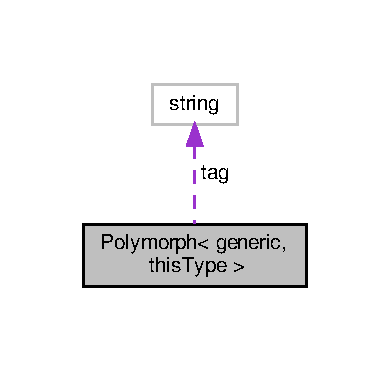
\includegraphics[width=187pt]{structPolymorph__coll__graph}
\end{center}
\end{figure}
\subsection*{Public Types}
\begin{DoxyCompactItemize}
\item 
\mbox{\Hypertarget{structPolymorph_a0d3d028703a1f6a992243ec98a1fd329}\label{structPolymorph_a0d3d028703a1f6a992243ec98a1fd329}} 
typedef this\+Type {\bfseries T}
\item 
\mbox{\Hypertarget{structPolymorph_ac1e1e1e20170b395bcd53fa5eb2e029a}\label{structPolymorph_ac1e1e1e20170b395bcd53fa5eb2e029a}} 
typedef generic {\bfseries G}
\item 
\mbox{\Hypertarget{structPolymorph_a0d3d028703a1f6a992243ec98a1fd329}\label{structPolymorph_a0d3d028703a1f6a992243ec98a1fd329}} 
typedef this\+Type {\bfseries T}
\item 
\mbox{\Hypertarget{structPolymorph_ac1e1e1e20170b395bcd53fa5eb2e029a}\label{structPolymorph_ac1e1e1e20170b395bcd53fa5eb2e029a}} 
typedef generic {\bfseries G}
\item 
\mbox{\Hypertarget{structPolymorph_a0d3d028703a1f6a992243ec98a1fd329}\label{structPolymorph_a0d3d028703a1f6a992243ec98a1fd329}} 
typedef this\+Type {\bfseries T}
\item 
\mbox{\Hypertarget{structPolymorph_ac1e1e1e20170b395bcd53fa5eb2e029a}\label{structPolymorph_ac1e1e1e20170b395bcd53fa5eb2e029a}} 
typedef generic {\bfseries G}
\end{DoxyCompactItemize}
\subsection*{Public Member Functions}
\begin{DoxyCompactItemize}
\item 
\mbox{\Hypertarget{structPolymorph_a112a9ce47d21c4d945b603481f04436a}\label{structPolymorph_a112a9ce47d21c4d945b603481f04436a}} 
{\bfseries Polymorph} (std\+::string t)
\item 
\mbox{\Hypertarget{structPolymorph_a7d44a14d2b725880a416a359de263813}\label{structPolymorph_a7d44a14d2b725880a416a359de263813}} 
void {\bfseries set\+New\+Type} (G $\ast$\&element)
\item 
\mbox{\Hypertarget{structPolymorph_a112a9ce47d21c4d945b603481f04436a}\label{structPolymorph_a112a9ce47d21c4d945b603481f04436a}} 
{\bfseries Polymorph} (std\+::string t)
\item 
\mbox{\Hypertarget{structPolymorph_a7d44a14d2b725880a416a359de263813}\label{structPolymorph_a7d44a14d2b725880a416a359de263813}} 
void {\bfseries set\+New\+Type} (G $\ast$\&element)
\item 
\mbox{\Hypertarget{structPolymorph_a112a9ce47d21c4d945b603481f04436a}\label{structPolymorph_a112a9ce47d21c4d945b603481f04436a}} 
{\bfseries Polymorph} (std\+::string t)
\item 
\mbox{\Hypertarget{structPolymorph_a7d44a14d2b725880a416a359de263813}\label{structPolymorph_a7d44a14d2b725880a416a359de263813}} 
void {\bfseries set\+New\+Type} (G $\ast$\&element)
\end{DoxyCompactItemize}
\subsection*{Public Attributes}
\begin{DoxyCompactItemize}
\item 
\mbox{\Hypertarget{structPolymorph_a1e47664581636ee02b594126d5a6d70c}\label{structPolymorph_a1e47664581636ee02b594126d5a6d70c}} 
std\+::string {\bfseries tag}
\end{DoxyCompactItemize}


\subsection{Detailed Description}
\subsubsection*{template$<$typename generic, typename this\+Type$>$\newline
struct Polymorph$<$ generic, this\+Type $>$}

This structure is for grouping information necessary for parsing out polymorphic objects from an X\+ML. This takes two template types, one for the base class, and one for the inheriting class. The constructor takes in a string which is used as a tag for finding values in the X\+ML 

The documentation for this struct was generated from the following file\+:\begin{DoxyCompactItemize}
\item 
/home/behnam/\+C\+U\+D\+A-\/\+U\+R\+B/src/util/Parse\+Interface.\+h\end{DoxyCompactItemize}

\hypertarget{classRectangularBuilding}{}\section{Rectangular\+Building Class Reference}
\label{classRectangularBuilding}\index{Rectangular\+Building@{Rectangular\+Building}}


Inheritance diagram for Rectangular\+Building\+:
\nopagebreak
\begin{figure}[H]
\begin{center}
\leavevmode
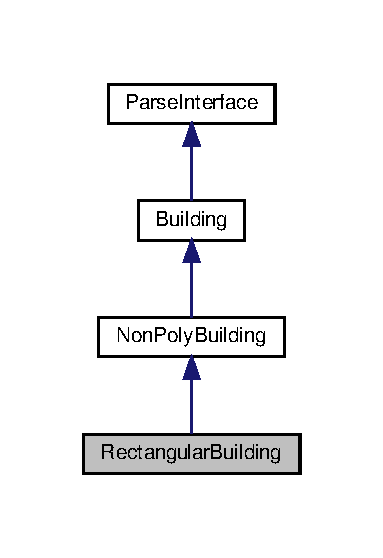
\includegraphics[width=184pt]{classRectangularBuilding__inherit__graph}
\end{center}
\end{figure}


Collaboration diagram for Rectangular\+Building\+:
\nopagebreak
\begin{figure}[H]
\begin{center}
\leavevmode
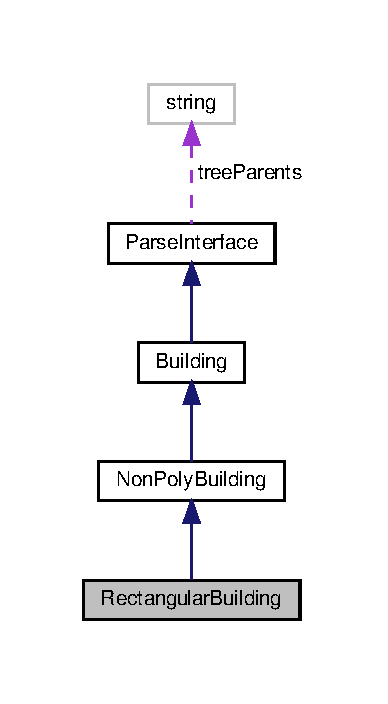
\includegraphics[width=186pt]{classRectangularBuilding__coll__graph}
\end{center}
\end{figure}
\subsection*{Public Member Functions}
\begin{DoxyCompactItemize}
\item 
\mbox{\Hypertarget{classRectangularBuilding_a5106fdd27a6eb098386f608e6eaf3135}\label{classRectangularBuilding_a5106fdd27a6eb098386f608e6eaf3135}} 
{\bfseries Rectangular\+Building} (float xfo, float yfo, float bh, float dx, float dy, float dz)
\item 
virtual void \hyperlink{classRectangularBuilding_adbc6b832c817fc06f9bc2e51561a7e81}{parse\+Values} ()
\item 
void \hyperlink{classRectangularBuilding_af690323c42b943b9a72ce6857b5e9ca0}{set\+Boundaries} (float dx, float dy, float dz, int nx, int ny, int nz, float $\ast$zm, float $\ast$e, float $\ast$f, float $\ast$g, float $\ast$h, float $\ast$m, float $\ast$n, int $\ast$icellflag)
\item 
void \hyperlink{classRectangularBuilding_ae2e0b496b0adf1b3e6961a42043f22c8}{set\+Cells} (int nx, int ny, int nz, int $\ast$icellflag, int $\ast$ibldflag, int ibuild)
\end{DoxyCompactItemize}
\subsection*{Additional Inherited Members}


\subsection{Member Function Documentation}
\mbox{\Hypertarget{classRectangularBuilding_adbc6b832c817fc06f9bc2e51561a7e81}\label{classRectangularBuilding_adbc6b832c817fc06f9bc2e51561a7e81}} 
\index{Rectangular\+Building@{Rectangular\+Building}!parse\+Values@{parse\+Values}}
\index{parse\+Values@{parse\+Values}!Rectangular\+Building@{Rectangular\+Building}}
\subsubsection{\texorpdfstring{parse\+Values()}{parseValues()}}
{\footnotesize\ttfamily virtual void Rectangular\+Building\+::parse\+Values (\begin{DoxyParamCaption}{ }\end{DoxyParamCaption})\hspace{0.3cm}{\ttfamily [inline]}, {\ttfamily [virtual]}}

Virtual function This is where we select what values we want to parse out of the xml file by calling the parseX functions above. 

Implements \hyperlink{classNonPolyBuilding_ace133756e0233d75b434fec5273b4414}{Non\+Poly\+Building}.

\mbox{\Hypertarget{classRectangularBuilding_af690323c42b943b9a72ce6857b5e9ca0}\label{classRectangularBuilding_af690323c42b943b9a72ce6857b5e9ca0}} 
\index{Rectangular\+Building@{Rectangular\+Building}!set\+Boundaries@{set\+Boundaries}}
\index{set\+Boundaries@{set\+Boundaries}!Rectangular\+Building@{Rectangular\+Building}}
\subsubsection{\texorpdfstring{set\+Boundaries()}{setBoundaries()}}
{\footnotesize\ttfamily void Rectangular\+Building\+::set\+Boundaries (\begin{DoxyParamCaption}\item[{float}]{dx,  }\item[{float}]{dy,  }\item[{float}]{dz,  }\item[{int}]{nx,  }\item[{int}]{ny,  }\item[{int}]{nz,  }\item[{float $\ast$}]{zm,  }\item[{float $\ast$}]{e,  }\item[{float $\ast$}]{f,  }\item[{float $\ast$}]{g,  }\item[{float $\ast$}]{h,  }\item[{float $\ast$}]{m,  }\item[{float $\ast$}]{n,  }\item[{int $\ast$}]{icellflag }\end{DoxyParamCaption})\hspace{0.3cm}{\ttfamily [inline]}}

Total number of cell-\/centered values in domain

Total number of face-\/centered values in domain

defining building and cut-\/cell indices

defining cells cut by building

Set cell index flag to cut-\/cell

defining building solid cells

Set cell index flag to building

defining ground solid cells

number of intersection points in each face of the cell

cut-\/cell index

intersection points hard-\/coded

area fraction coeeficient

calculate area fraction coeeficient for each face of the cut-\/cell

Assign solver coefficients

Wall bellow

Wall above

Wall in back

Wall in front

Wall on right

Wall on left \mbox{\Hypertarget{classRectangularBuilding_ae2e0b496b0adf1b3e6961a42043f22c8}\label{classRectangularBuilding_ae2e0b496b0adf1b3e6961a42043f22c8}} 
\index{Rectangular\+Building@{Rectangular\+Building}!set\+Cells@{set\+Cells}}
\index{set\+Cells@{set\+Cells}!Rectangular\+Building@{Rectangular\+Building}}
\subsubsection{\texorpdfstring{set\+Cells()}{setCells()}}
{\footnotesize\ttfamily void Rectangular\+Building\+::set\+Cells (\begin{DoxyParamCaption}\item[{int}]{nx,  }\item[{int}]{ny,  }\item[{int}]{nz,  }\item[{int $\ast$}]{icellflag,  }\item[{int $\ast$}]{ibldflag,  }\item[{int}]{ibuild }\end{DoxyParamCaption})\hspace{0.3cm}{\ttfamily [inline]}}

Lineralized index for cell centered values

Set cell index flag to cut-\/cell

Lineralized index for cell centered values

Set cell index flag to building 

The documentation for this class was generated from the following file\+:\begin{DoxyCompactItemize}
\item 
/home/behnam/\+C\+U\+D\+A-\/\+U\+R\+B/src/Rectangular\+Building.\+h\end{DoxyCompactItemize}

\hypertarget{classRoot}{}\section{Root Class Reference}
\label{classRoot}\index{Root@{Root}}


Inheritance diagram for Root\+:
\nopagebreak
\begin{figure}[H]
\begin{center}
\leavevmode
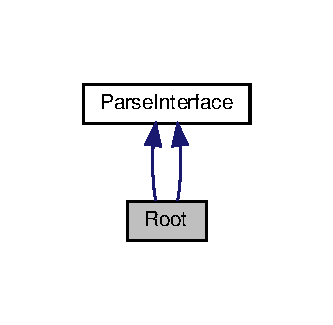
\includegraphics[width=160pt]{classRoot__inherit__graph}
\end{center}
\end{figure}


Collaboration diagram for Root\+:
\nopagebreak
\begin{figure}[H]
\begin{center}
\leavevmode
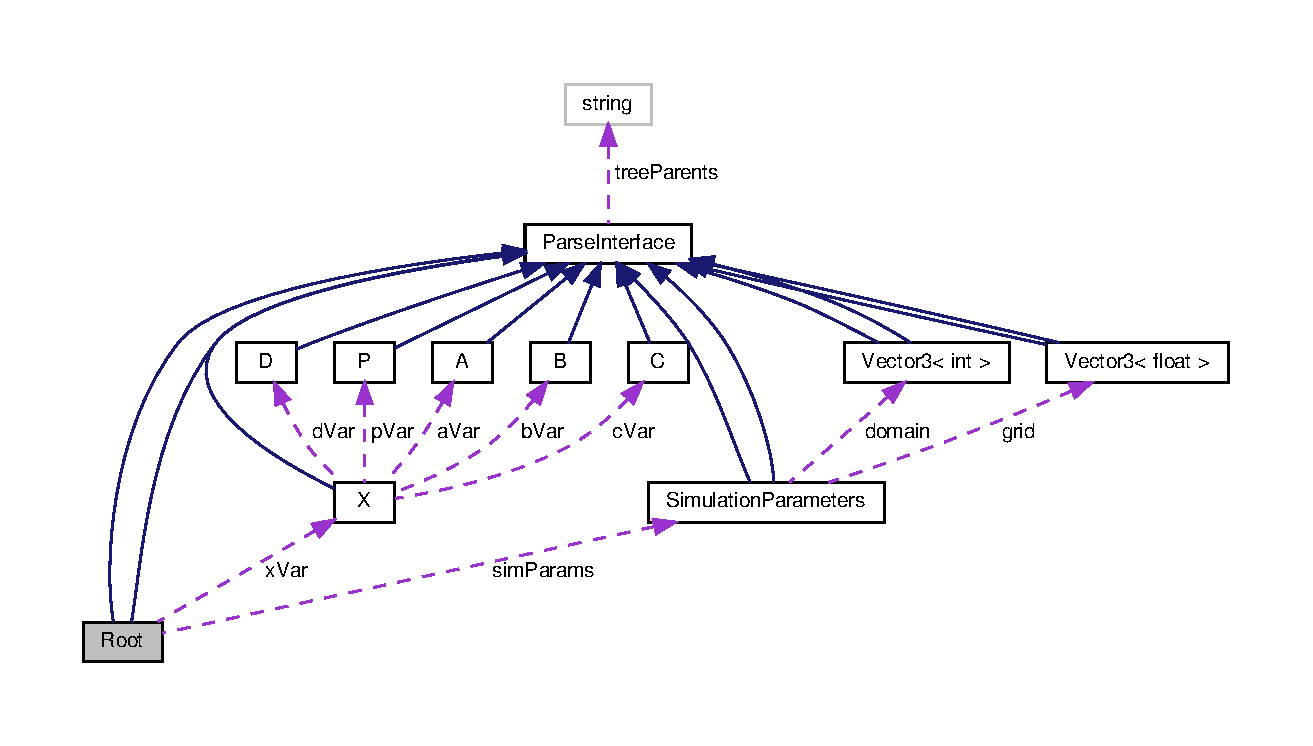
\includegraphics[width=350pt]{classRoot__coll__graph}
\end{center}
\end{figure}
\subsection*{Public Member Functions}
\begin{DoxyCompactItemize}
\item 
void \hyperlink{classRoot_ade0eb65da55fa8c045a76bcf1fb16009}{parse\+Values} ()
\item 
void \hyperlink{classRoot_ade0eb65da55fa8c045a76bcf1fb16009}{parse\+Values} ()
\end{DoxyCompactItemize}
\subsection*{Public Attributes}
\begin{DoxyCompactItemize}
\item 
\mbox{\Hypertarget{classRoot_aa61fa8f78e32674c07681894d1dd3a12}\label{classRoot_aa61fa8f78e32674c07681894d1dd3a12}} 
\hyperlink{classX}{X} $\ast$ {\bfseries x\+Var}
\item 
\mbox{\Hypertarget{classRoot_a9234ed2debae0233778343218393f9b2}\label{classRoot_a9234ed2debae0233778343218393f9b2}} 
\hyperlink{classSimulationParameters}{Simulation\+Parameters} $\ast$ {\bfseries sim\+Params}
\end{DoxyCompactItemize}
\subsection*{Additional Inherited Members}


\subsection{Member Function Documentation}
\mbox{\Hypertarget{classRoot_ade0eb65da55fa8c045a76bcf1fb16009}\label{classRoot_ade0eb65da55fa8c045a76bcf1fb16009}} 
\index{Root@{Root}!parse\+Values@{parse\+Values}}
\index{parse\+Values@{parse\+Values}!Root@{Root}}
\subsubsection{\texorpdfstring{parse\+Values()}{parseValues()}\hspace{0.1cm}{\footnotesize\ttfamily [1/2]}}
{\footnotesize\ttfamily void Root\+::parse\+Values (\begin{DoxyParamCaption}{ }\end{DoxyParamCaption})\hspace{0.3cm}{\ttfamily [inline]}, {\ttfamily [virtual]}}

Virtual function This is where we select what values we want to parse out of the xml file by calling the parseX functions above. 

Implements \hyperlink{classParseInterface_afca32108192ba0997c9e5a78189b0cbc}{Parse\+Interface}.

\mbox{\Hypertarget{classRoot_ade0eb65da55fa8c045a76bcf1fb16009}\label{classRoot_ade0eb65da55fa8c045a76bcf1fb16009}} 
\index{Root@{Root}!parse\+Values@{parse\+Values}}
\index{parse\+Values@{parse\+Values}!Root@{Root}}
\subsubsection{\texorpdfstring{parse\+Values()}{parseValues()}\hspace{0.1cm}{\footnotesize\ttfamily [2/2]}}
{\footnotesize\ttfamily void Root\+::parse\+Values (\begin{DoxyParamCaption}{ }\end{DoxyParamCaption})\hspace{0.3cm}{\ttfamily [inline]}, {\ttfamily [virtual]}}

Virtual function This is where we select what values we want to parse out of the xml file by calling the parseX functions above. 

Implements \hyperlink{classParseInterface_afca32108192ba0997c9e5a78189b0cbc}{Parse\+Interface}.



The documentation for this class was generated from the following file\+:\begin{DoxyCompactItemize}
\item 
/home/behnam/\+C\+U\+D\+A-\/\+U\+R\+B/xml\+Testing/Root.\+h\end{DoxyCompactItemize}

\hypertarget{classSensor}{}\section{Sensor Class Reference}
\label{classSensor}\index{Sensor@{Sensor}}


Inheritance diagram for Sensor\+:
\nopagebreak
\begin{figure}[H]
\begin{center}
\leavevmode
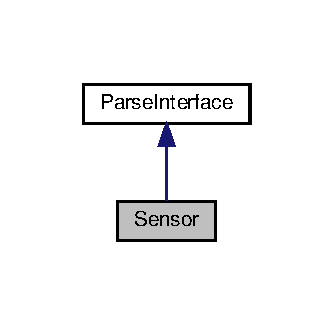
\includegraphics[width=160pt]{classSensor__inherit__graph}
\end{center}
\end{figure}


Collaboration diagram for Sensor\+:
\nopagebreak
\begin{figure}[H]
\begin{center}
\leavevmode
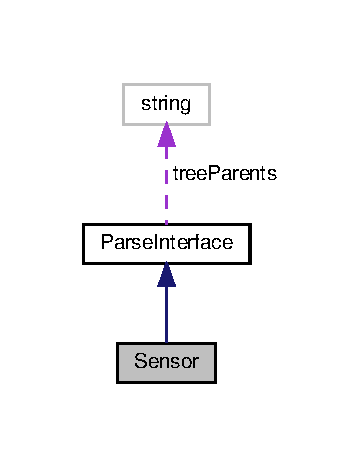
\includegraphics[width=174pt]{classSensor__coll__graph}
\end{center}
\end{figure}
\subsection*{Public Member Functions}
\begin{DoxyCompactItemize}
\item 
virtual void \hyperlink{classSensor_a570a911466a9fd98894f7c2f2abaf103}{parse\+Values} ()
\end{DoxyCompactItemize}
\subsection*{Public Attributes}
\begin{DoxyCompactItemize}
\item 
\mbox{\Hypertarget{classSensor_a828c198acfd09e73bccf793b42298f3c}\label{classSensor_a828c198acfd09e73bccf793b42298f3c}} 
int {\bfseries site\+\_\+blayer\+\_\+flag}
\item 
\mbox{\Hypertarget{classSensor_a7e026ca937dc83f3787d47bda5a1da88}\label{classSensor_a7e026ca937dc83f3787d47bda5a1da88}} 
float {\bfseries site\+\_\+one\+\_\+overL}
\item 
\mbox{\Hypertarget{classSensor_a9e5d9067d8fbce64ebef4b7f296e2cd2}\label{classSensor_a9e5d9067d8fbce64ebef4b7f296e2cd2}} 
float {\bfseries site\+\_\+xcoord}
\item 
\mbox{\Hypertarget{classSensor_af04a68f318fa7a67350eb16ae1ae9a20}\label{classSensor_af04a68f318fa7a67350eb16ae1ae9a20}} 
float {\bfseries site\+\_\+ycoord}
\item 
\mbox{\Hypertarget{classSensor_a230269e79efba1abea972937db7e9154}\label{classSensor_a230269e79efba1abea972937db7e9154}} 
float {\bfseries site\+\_\+wind\+\_\+dir}
\item 
\mbox{\Hypertarget{classSensor_afa438ddacfd4d2335d8cad89153da94a}\label{classSensor_afa438ddacfd4d2335d8cad89153da94a}} 
float {\bfseries site\+\_\+z0}
\item 
\mbox{\Hypertarget{classSensor_ae620715b6b61af219845bf586d4be6ef}\label{classSensor_ae620715b6b61af219845bf586d4be6ef}} 
float {\bfseries site\+\_\+z\+\_\+ref}
\item 
\mbox{\Hypertarget{classSensor_a74b406df28d5e1153cc63b591e6ed8e7}\label{classSensor_a74b406df28d5e1153cc63b591e6ed8e7}} 
float {\bfseries site\+\_\+\+U\+\_\+ref}
\end{DoxyCompactItemize}
\subsection*{Additional Inherited Members}


\subsection{Member Function Documentation}
\mbox{\Hypertarget{classSensor_a570a911466a9fd98894f7c2f2abaf103}\label{classSensor_a570a911466a9fd98894f7c2f2abaf103}} 
\index{Sensor@{Sensor}!parse\+Values@{parse\+Values}}
\index{parse\+Values@{parse\+Values}!Sensor@{Sensor}}
\subsubsection{\texorpdfstring{parse\+Values()}{parseValues()}}
{\footnotesize\ttfamily virtual void Sensor\+::parse\+Values (\begin{DoxyParamCaption}{ }\end{DoxyParamCaption})\hspace{0.3cm}{\ttfamily [inline]}, {\ttfamily [virtual]}}

Virtual function This is where we select what values we want to parse out of the xml file by calling the parseX functions above. 

Implements \hyperlink{classParseInterface_afca32108192ba0997c9e5a78189b0cbc}{Parse\+Interface}.



The documentation for this class was generated from the following file\+:\begin{DoxyCompactItemize}
\item 
/home/behnam/\+C\+U\+D\+A-\/\+U\+R\+B/src/Sensor.\+h\end{DoxyCompactItemize}

\hypertarget{classSimulationParameters}{}\section{Simulation\+Parameters Class Reference}
\label{classSimulationParameters}\index{Simulation\+Parameters@{Simulation\+Parameters}}


Inheritance diagram for Simulation\+Parameters\+:
\nopagebreak
\begin{figure}[H]
\begin{center}
\leavevmode
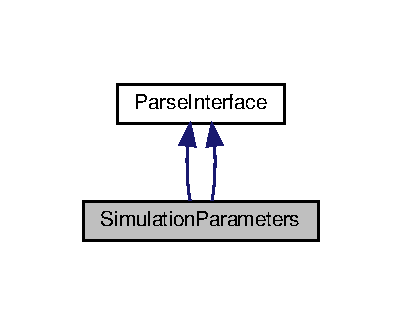
\includegraphics[width=193pt]{classSimulationParameters__inherit__graph}
\end{center}
\end{figure}


Collaboration diagram for Simulation\+Parameters\+:
\nopagebreak
\begin{figure}[H]
\begin{center}
\leavevmode
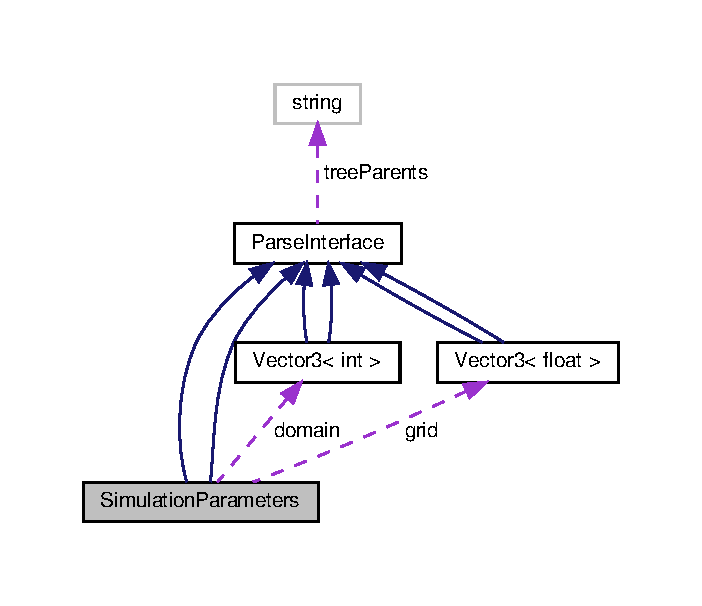
\includegraphics[width=337pt]{classSimulationParameters__coll__graph}
\end{center}
\end{figure}
\subsection*{Public Member Functions}
\begin{DoxyCompactItemize}
\item 
virtual void \hyperlink{classSimulationParameters_a306c6d373794f5186beec9026f56845c}{parse\+Values} ()
\item 
virtual void \hyperlink{classSimulationParameters_a306c6d373794f5186beec9026f56845c}{parse\+Values} ()
\end{DoxyCompactItemize}
\subsection*{Public Attributes}
\begin{DoxyCompactItemize}
\item 
\mbox{\Hypertarget{classSimulationParameters_a35f2a333d5d019425a16579a34dd1956}\label{classSimulationParameters_a35f2a333d5d019425a16579a34dd1956}} 
\hyperlink{classVector3}{Vector3}$<$ int $>$ $\ast$ {\bfseries domain}
\item 
\mbox{\Hypertarget{classSimulationParameters_acc14170c2c36cafb307be92674b1cc39}\label{classSimulationParameters_acc14170c2c36cafb307be92674b1cc39}} 
\hyperlink{classVector3}{Vector3}$<$ float $>$ $\ast$ {\bfseries grid}
\item 
\mbox{\Hypertarget{classSimulationParameters_a9502bf08efbca3b43d2c1a1ec3ceb80b}\label{classSimulationParameters_a9502bf08efbca3b43d2c1a1ec3ceb80b}} 
int {\bfseries vertical\+Stretching}
\item 
\mbox{\Hypertarget{classSimulationParameters_a54499bd3028a6488dbfc59b0d6471444}\label{classSimulationParameters_a54499bd3028a6488dbfc59b0d6471444}} 
int {\bfseries total\+Time\+Increments}
\item 
\mbox{\Hypertarget{classSimulationParameters_a2d4701335d74b394a7a25b86371f8337}\label{classSimulationParameters_a2d4701335d74b394a7a25b86371f8337}} 
int {\bfseries U\+T\+C\+Conversion}
\item 
\mbox{\Hypertarget{classSimulationParameters_ae96bebaef08a0234f1e37617dd204a7e}\label{classSimulationParameters_ae96bebaef08a0234f1e37617dd204a7e}} 
float {\bfseries Epoch}
\item 
\mbox{\Hypertarget{classSimulationParameters_a938d73fe33bd42d8c180775e4a52bf9e}\label{classSimulationParameters_a938d73fe33bd42d8c180775e4a52bf9e}} 
int {\bfseries rooftop\+Flag}
\item 
\mbox{\Hypertarget{classSimulationParameters_a99eca86110cced2344b7732e973eb00f}\label{classSimulationParameters_a99eca86110cced2344b7732e973eb00f}} 
int {\bfseries upwind\+Cavity\+Flag}
\item 
\mbox{\Hypertarget{classSimulationParameters_ac4058de8aafc45132ba44bb8dcde837d}\label{classSimulationParameters_ac4058de8aafc45132ba44bb8dcde837d}} 
int {\bfseries street\+Canyon\+Flag}
\item 
\mbox{\Hypertarget{classSimulationParameters_a068cb2cac14b6a4f55a79e6632402386}\label{classSimulationParameters_a068cb2cac14b6a4f55a79e6632402386}} 
int {\bfseries street\+Intersection\+Flag}
\item 
\mbox{\Hypertarget{classSimulationParameters_a58062697b8cac9513d96ae2d57d876fb}\label{classSimulationParameters_a58062697b8cac9513d96ae2d57d876fb}} 
int {\bfseries wake\+Flag}
\item 
\mbox{\Hypertarget{classSimulationParameters_aefeb040f366e72cc8ed36f64e21aa0f5}\label{classSimulationParameters_aefeb040f366e72cc8ed36f64e21aa0f5}} 
int {\bfseries sidewall\+Flag}
\item 
\mbox{\Hypertarget{classSimulationParameters_a91db3728301ea103b267a56f80e5b499}\label{classSimulationParameters_a91db3728301ea103b267a56f80e5b499}} 
int {\bfseries max\+Iterations}
\item 
\mbox{\Hypertarget{classSimulationParameters_a483bbd3e82383e19813534e809d483d3}\label{classSimulationParameters_a483bbd3e82383e19813534e809d483d3}} 
int {\bfseries residual\+Reduction}
\item 
\mbox{\Hypertarget{classSimulationParameters_af8404a5cd90e708ac5d38b1866bb455b}\label{classSimulationParameters_af8404a5cd90e708ac5d38b1866bb455b}} 
float {\bfseries domain\+Rotation}
\item 
\mbox{\Hypertarget{classSimulationParameters_a592d32d60df729d28118cc71512d4b3d}\label{classSimulationParameters_a592d32d60df729d28118cc71512d4b3d}} 
int {\bfseries U\+T\+MX}
\item 
\mbox{\Hypertarget{classSimulationParameters_a98f6060af3b91e179c18f1c1effdb522}\label{classSimulationParameters_a98f6060af3b91e179c18f1c1effdb522}} 
int {\bfseries U\+T\+MY}
\item 
\mbox{\Hypertarget{classSimulationParameters_a53fa9d9457e6bc6b8f6a343da584b665}\label{classSimulationParameters_a53fa9d9457e6bc6b8f6a343da584b665}} 
int {\bfseries U\+T\+M\+Zone}
\item 
\mbox{\Hypertarget{classSimulationParameters_a063c83eedfbd7402d7dfab1e5881df66}\label{classSimulationParameters_a063c83eedfbd7402d7dfab1e5881df66}} 
int {\bfseries U\+T\+M\+Zone\+Letter}
\item 
\mbox{\Hypertarget{classSimulationParameters_a1b963497ee10962f6a5528f1a940f7fe}\label{classSimulationParameters_a1b963497ee10962f6a5528f1a940f7fe}} 
std\+::vector$<$ float $>$ {\bfseries dz\+Array}
\end{DoxyCompactItemize}
\subsection*{Additional Inherited Members}


\subsection{Member Function Documentation}
\mbox{\Hypertarget{classSimulationParameters_a306c6d373794f5186beec9026f56845c}\label{classSimulationParameters_a306c6d373794f5186beec9026f56845c}} 
\index{Simulation\+Parameters@{Simulation\+Parameters}!parse\+Values@{parse\+Values}}
\index{parse\+Values@{parse\+Values}!Simulation\+Parameters@{Simulation\+Parameters}}
\subsubsection{\texorpdfstring{parse\+Values()}{parseValues()}\hspace{0.1cm}{\footnotesize\ttfamily [1/2]}}
{\footnotesize\ttfamily virtual void Simulation\+Parameters\+::parse\+Values (\begin{DoxyParamCaption}{ }\end{DoxyParamCaption})\hspace{0.3cm}{\ttfamily [inline]}, {\ttfamily [virtual]}}

Virtual function This is where we select what values we want to parse out of the xml file by calling the parseX functions above. 

Implements \hyperlink{classParseInterface_afca32108192ba0997c9e5a78189b0cbc}{Parse\+Interface}.

\mbox{\Hypertarget{classSimulationParameters_a306c6d373794f5186beec9026f56845c}\label{classSimulationParameters_a306c6d373794f5186beec9026f56845c}} 
\index{Simulation\+Parameters@{Simulation\+Parameters}!parse\+Values@{parse\+Values}}
\index{parse\+Values@{parse\+Values}!Simulation\+Parameters@{Simulation\+Parameters}}
\subsubsection{\texorpdfstring{parse\+Values()}{parseValues()}\hspace{0.1cm}{\footnotesize\ttfamily [2/2]}}
{\footnotesize\ttfamily virtual void Simulation\+Parameters\+::parse\+Values (\begin{DoxyParamCaption}{ }\end{DoxyParamCaption})\hspace{0.3cm}{\ttfamily [inline]}, {\ttfamily [virtual]}}

Virtual function This is where we select what values we want to parse out of the xml file by calling the parseX functions above. 

Implements \hyperlink{classParseInterface_afca32108192ba0997c9e5a78189b0cbc}{Parse\+Interface}.



The documentation for this class was generated from the following file\+:\begin{DoxyCompactItemize}
\item 
/home/behnam/\+C\+U\+D\+A-\/\+U\+R\+B/src/Simulation\+Parameters.\+h\end{DoxyCompactItemize}

\hypertarget{classSolver}{}\section{Solver Class Reference}
\label{classSolver}\index{Solver@{Solver}}


{\ttfamily \#include $<$Solver.\+h$>$}



Inheritance diagram for Solver\+:
\nopagebreak
\begin{figure}[H]
\begin{center}
\leavevmode
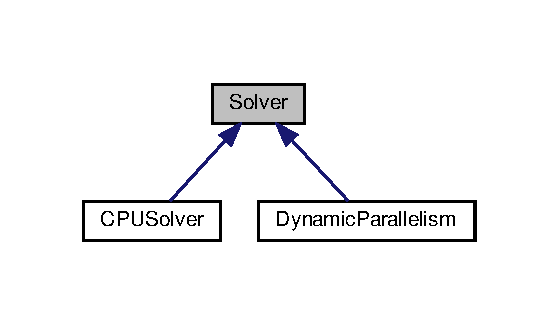
\includegraphics[width=268pt]{classSolver__inherit__graph}
\end{center}
\end{figure}


Collaboration diagram for Solver\+:
\nopagebreak
\begin{figure}[H]
\begin{center}
\leavevmode
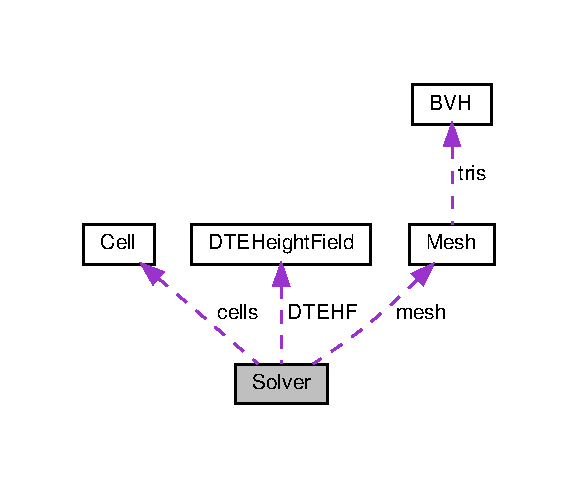
\includegraphics[width=278pt]{classSolver__coll__graph}
\end{center}
\end{figure}
\subsection*{Public Member Functions}
\begin{DoxyCompactItemize}
\item 
\hyperlink{classSolver_a0df0752d39f016c7dc636d8c46274218}{Solver} (\hyperlink{classURBInputData}{U\+R\+B\+Input\+Data} $\ast$U\+ID, \hyperlink{classDTEHeightField}{D\+T\+E\+Height\+Field} $\ast$D\+T\+E\+HF)
\item 
\mbox{\Hypertarget{classSolver_ad004f38b8aff33fa13a8971f87f7816e}\label{classSolver_ad004f38b8aff33fa13a8971f87f7816e}} 
virtual void {\bfseries solve} (\hyperlink{classNetCDFData}{Net\+C\+D\+F\+Data} $\ast$netcdf\+Dat, bool solve\+Wind)=0
\item 
void \hyperlink{classSolver_a66fa054cbf52fd6c184386fe11f9cadf}{define\+Walls} (int $\ast$i\+Cell\+Flag, float $\ast$n, float $\ast$m, float $\ast$f, float $\ast$\hyperlink{classSolver_ab65a76ec3befd44f11e817fdef8f47a6}{e}, float $\ast$h, float $\ast$g)
\item 
\mbox{\Hypertarget{classSolver_af815849a5dda94feb2a5a0e5afa3e5a2}\label{classSolver_af815849a5dda94feb2a5a0e5afa3e5a2}} 
void {\bfseries up\+Wind} (\hyperlink{classBuilding}{Building} $\ast$build, int $\ast$i\+Cell\+Flag, double $\ast$\hyperlink{classSolver_aaf60f18219d1d08959b9a6fa209d5e17}{u0}, double $\ast$v0, double $\ast$w0, float $\ast$z, float $\ast$zm)
\item 
\mbox{\Hypertarget{classSolver_aa74c027e6f75376d459cecbfd71dbc2f}\label{classSolver_aa74c027e6f75376d459cecbfd71dbc2f}} 
void {\bfseries relief\+Wake} (\hyperlink{classNonPolyBuilding}{Non\+Poly\+Building} $\ast$build, float $\ast$\hyperlink{classSolver_aaf60f18219d1d08959b9a6fa209d5e17}{u0}, float $\ast$v0)
\end{DoxyCompactItemize}
\subsection*{Protected Member Functions}
\begin{DoxyCompactItemize}
\item 
\mbox{\Hypertarget{classSolver_a4380db2e63e45a27b1cae8d9558f004d}\label{classSolver_a4380db2e63e45a27b1cae8d9558f004d}} 
void {\bfseries print\+Progress} (float percentage)
\end{DoxyCompactItemize}
\subsection*{Protected Attributes}
\begin{DoxyCompactItemize}
\item 
\mbox{\Hypertarget{classSolver_aae65c28682a9953c5164cd8c6da3d69c}\label{classSolver_aae65c28682a9953c5164cd8c6da3d69c}} 
int {\bfseries nx}
\item 
\mbox{\Hypertarget{classSolver_a1f154e748c539e4cfcee150c7e155daf}\label{classSolver_a1f154e748c539e4cfcee150c7e155daf}} 
int {\bfseries ny}
\item 
int \hyperlink{classSolver_a4312c5a1ff7a5eba3eb8d7ef3fed0190}{nz}
\item 
\mbox{\Hypertarget{classSolver_a4a3e239b59c3822b17edae555b7683d7}\label{classSolver_a4a3e239b59c3822b17edae555b7683d7}} 
float {\bfseries dx}
\item 
\mbox{\Hypertarget{classSolver_a137aa51312a07b0ce69959dccc4ab7b6}\label{classSolver_a137aa51312a07b0ce69959dccc4ab7b6}} 
float {\bfseries dy}
\item 
float \hyperlink{classSolver_aed4366cb221b3429a878cb39a06b0ef4}{dz}
\item 
float \hyperlink{classSolver_acca22a72409a3ccff8662d0000358512}{dxy}
\item 
\mbox{\Hypertarget{classSolver_a83c7c4b749580980db91770e88b2fcf5}\label{classSolver_a83c7c4b749580980db91770e88b2fcf5}} 
std\+::vector$<$ float $>$ {\bfseries dz\+Array}
\item 
\mbox{\Hypertarget{classSolver_a4cc407bf68dc76310521a7b347e39dc0}\label{classSolver_a4cc407bf68dc76310521a7b347e39dc0}} 
std\+::vector$<$ float $>$ {\bfseries zm}
\item 
\mbox{\Hypertarget{classSolver_ad06fb03e479e8c41b1960f21e510c0d0}\label{classSolver_ad06fb03e479e8c41b1960f21e510c0d0}} 
std\+::vector$<$ float $>$ {\bfseries x}
\item 
\mbox{\Hypertarget{classSolver_aa70241bd5d16502b7becb591dc141ec3}\label{classSolver_aa70241bd5d16502b7becb591dc141ec3}} 
std\+::vector$<$ float $>$ {\bfseries y}
\item 
\mbox{\Hypertarget{classSolver_a179243358326a5c867706192597b30f3}\label{classSolver_a179243358326a5c867706192597b30f3}} 
std\+::vector$<$ float $>$ {\bfseries z}
\item 
int \hyperlink{classSolver_aa42a6832b9dd82be64b07071135b69e8}{itermax}
\item 
int \hyperlink{classSolver_a0edd9bd90200b40133cc007c9f9600bb}{num\+\_\+sites}
\item 
std\+::vector$<$ int $>$ \hyperlink{classSolver_ad28319be4f9915bec3840aadd083c2ae}{site\+\_\+blayer\+\_\+flag}
\item 
std\+::vector$<$ float $>$ \hyperlink{classSolver_ad5f6e755ca6e125ae1499afe1930dfcf}{site\+\_\+one\+\_\+overL}
\item 
std\+::vector$<$ float $>$ \hyperlink{classSolver_a431d4f3051f3c29aabccb5e539e91f4d}{site\+\_\+xcoord}
\item 
std\+::vector$<$ float $>$ \hyperlink{classSolver_a00a819ad1ff7e520b23488a25f43d729}{site\+\_\+ycoord}
\item 
std\+::vector$<$ float $>$ \hyperlink{classSolver_a8c9d9b52656069625d10ba854680f118}{site\+\_\+wind\+\_\+dir}
\item 
std\+::vector$<$ float $>$ \hyperlink{classSolver_a7ca18ea25f9117d2c43f7ea7cf1569e6}{site\+\_\+z0}
\item 
std\+::vector$<$ float $>$ \hyperlink{classSolver_a838b82880aa58582918678eb7b969938}{site\+\_\+z\+\_\+ref}
\item 
std\+::vector$<$ float $>$ \hyperlink{classSolver_adae403dd4db1cf42265cfd74f3ff9452}{site\+\_\+\+U\+\_\+ref}
\item 
\mbox{\Hypertarget{classSolver_ab65a76ec3befd44f11e817fdef8f47a6}\label{classSolver_ab65a76ec3befd44f11e817fdef8f47a6}} 
std\+::vector$<$ float $>$ \hyperlink{classSolver_ab65a76ec3befd44f11e817fdef8f47a6}{e}
\begin{DoxyCompactList}\small\item\em Declare coefficients for S\+OR solver. \end{DoxyCompactList}\item 
\mbox{\Hypertarget{classSolver_ab54b33f50a45b825f4539384f35f61d9}\label{classSolver_ab54b33f50a45b825f4539384f35f61d9}} 
std\+::vector$<$ float $>$ {\bfseries f}
\item 
\mbox{\Hypertarget{classSolver_a26c3952745b8244e167a6b92e7a4a3c3}\label{classSolver_a26c3952745b8244e167a6b92e7a4a3c3}} 
std\+::vector$<$ float $>$ {\bfseries g}
\item 
\mbox{\Hypertarget{classSolver_a17a3e816297c81a3d4a7af3820884774}\label{classSolver_a17a3e816297c81a3d4a7af3820884774}} 
std\+::vector$<$ float $>$ {\bfseries h}
\item 
\mbox{\Hypertarget{classSolver_ae5e24f7a9bdda4c664244cb11316feef}\label{classSolver_ae5e24f7a9bdda4c664244cb11316feef}} 
std\+::vector$<$ float $>$ {\bfseries m}
\item 
\mbox{\Hypertarget{classSolver_a53c23907e08c2ccdffbd9001b16a72e2}\label{classSolver_a53c23907e08c2ccdffbd9001b16a72e2}} 
std\+::vector$<$ float $>$ {\bfseries n}
\item 
\mbox{\Hypertarget{classSolver_aaf60f18219d1d08959b9a6fa209d5e17}\label{classSolver_aaf60f18219d1d08959b9a6fa209d5e17}} 
std\+::vector$<$ double $>$ \hyperlink{classSolver_aaf60f18219d1d08959b9a6fa209d5e17}{u0}
\begin{DoxyCompactList}\small\item\em Declaration of initial wind components (u0,v0,w0) \end{DoxyCompactList}\item 
\mbox{\Hypertarget{classSolver_ac5900dc7c2afdaaea09fbadb1e415276}\label{classSolver_ac5900dc7c2afdaaea09fbadb1e415276}} 
std\+::vector$<$ double $>$ {\bfseries v0}
\item 
\mbox{\Hypertarget{classSolver_afcf2572409568d3056b396a4b3ceae54}\label{classSolver_afcf2572409568d3056b396a4b3ceae54}} 
std\+::vector$<$ double $>$ {\bfseries w0}
\item 
std\+::vector$<$ double $>$ \hyperlink{classSolver_aaca74be9e1a11be0c7a480c4202670e7}{R}
\item 
\mbox{\Hypertarget{classSolver_a4ef34a205c0f10ac6aebe746865c5560}\label{classSolver_a4ef34a205c0f10ac6aebe746865c5560}} 
std\+::vector$<$ double $>$ \hyperlink{classSolver_a4ef34a205c0f10ac6aebe746865c5560}{u}
\begin{DoxyCompactList}\small\item\em Declaration of final velocity field components (u,v,w) \end{DoxyCompactList}\item 
\mbox{\Hypertarget{classSolver_ae0521e44d6759661ee87b8cad4d8880c}\label{classSolver_ae0521e44d6759661ee87b8cad4d8880c}} 
std\+::vector$<$ double $>$ {\bfseries v}
\item 
\mbox{\Hypertarget{classSolver_afab3c620a5ee2755f725347a834d8689}\label{classSolver_afab3c620a5ee2755f725347a834d8689}} 
std\+::vector$<$ double $>$ {\bfseries w}
\item 
\mbox{\Hypertarget{classSolver_a7cbf1a351c061c4d33e977ae95e246ef}\label{classSolver_a7cbf1a351c061c4d33e977ae95e246ef}} 
std\+::vector$<$ double $>$ \hyperlink{classSolver_a7cbf1a351c061c4d33e977ae95e246ef}{lambda}
\begin{DoxyCompactList}\small\item\em Declaration of Lagrange multipliers. \end{DoxyCompactList}\item 
\mbox{\Hypertarget{classSolver_a479deb1cb4d561d0389fc9d14aa0fc0d}\label{classSolver_a479deb1cb4d561d0389fc9d14aa0fc0d}} 
std\+::vector$<$ double $>$ {\bfseries lambda\+\_\+old}
\item 
\mbox{\Hypertarget{classSolver_af7773bf4c9fce880f071bd47ba2bcf28}\label{classSolver_af7773bf4c9fce880f071bd47ba2bcf28}} 
std\+::vector$<$ int $>$ {\bfseries icellflag}
\item 
\mbox{\Hypertarget{classSolver_a3c7a2b93b76bc0c219740988e8f0bbe3}\label{classSolver_a3c7a2b93b76bc0c219740988e8f0bbe3}} 
float \hyperlink{classSolver_a3c7a2b93b76bc0c219740988e8f0bbe3}{max\+\_\+velmag}
\begin{DoxyCompactList}\small\item\em \hyperlink{classCell}{Cell} index flag (0 = building, 1 = fluid) \end{DoxyCompactList}\item 
\mbox{\Hypertarget{classSolver_a560d2a46322206e831c0395f3933f1b0}\label{classSolver_a560d2a46322206e831c0395f3933f1b0}} 
std\+::vector$<$ \hyperlink{classBuilding}{Building} $\ast$ $>$ {\bfseries buildings}
\item 
\mbox{\Hypertarget{classSolver_a9b516765134fb4193329639761924cf7}\label{classSolver_a9b516765134fb4193329639761924cf7}} 
\hyperlink{classMesh}{Mesh} $\ast$ {\bfseries mesh}
\item 
int \hyperlink{classSolver_ada5e48b402bea1092dc90d2fa7d374e9}{rooftop\+Flag}
\item 
int \hyperlink{classSolver_a597d486a292558f5f55db306eeec42d1}{upwind\+Cavity\+Flag}
\item 
int \hyperlink{classSolver_af05b7600810c10dbf97b926bd67b71da}{street\+Canyon\+Flag}
\item 
int \hyperlink{classSolver_ad30bcedb245dc79e937cbf7776fc27d7}{street\+Intersection\+Flag}
\item 
int \hyperlink{classSolver_a5de7954b3723e984ef9c4963dfedcb04}{wake\+Flag}
\item 
int \hyperlink{classSolver_a243552b62125c493cd0f08f3bbfe3723}{sidewall\+Flag}
\item 
\mbox{\Hypertarget{classSolver_a21a65352d2b9fe246309a54a1fb916c0}\label{classSolver_a21a65352d2b9fe246309a54a1fb916c0}} 
\hyperlink{classCell}{Cell} $\ast$ {\bfseries cells}
\item 
\mbox{\Hypertarget{classSolver_a0a19a30f249bc14ce15915c2cb533f7f}\label{classSolver_a0a19a30f249bc14ce15915c2cb533f7f}} 
\hyperlink{classDTEHeightField}{D\+T\+E\+Height\+Field} $\ast$ {\bfseries D\+T\+E\+HF}
\item 
\mbox{\Hypertarget{classSolver_a65a58db8e3b6ff0938f297d959298441}\label{classSolver_a65a58db8e3b6ff0938f297d959298441}} 
float {\bfseries z0}
\item 
const int \hyperlink{classSolver_a1dba41a0d2c04b18cf121e2730a5d2f0}{alpha1} = 1
\item 
const int \hyperlink{classSolver_ac6cd00ae8ed99b0375a15fd0973d674b}{alpha2} = 1
\item 
\mbox{\Hypertarget{classSolver_af870716dd37bbf5710fde9c9da2c450a}\label{classSolver_af870716dd37bbf5710fde9c9da2c450a}} 
const float {\bfseries eta} = pow(\hyperlink{classSolver_a1dba41a0d2c04b18cf121e2730a5d2f0}{alpha1}/\hyperlink{classSolver_ac6cd00ae8ed99b0375a15fd0973d674b}{alpha2}, 2.\+0)
\item 
\mbox{\Hypertarget{classSolver_a5744d5828cc41b1981141d780c30b1c4}\label{classSolver_a5744d5828cc41b1981141d780c30b1c4}} 
const float {\bfseries A} = pow(dx/dy, 2.\+0)
\item 
\mbox{\Hypertarget{classSolver_a0f0aa4fa9d7a1a92453db21b17ad73db}\label{classSolver_a0f0aa4fa9d7a1a92453db21b17ad73db}} 
const float {\bfseries B} = eta$\ast$pow(dx/\hyperlink{classSolver_aed4366cb221b3429a878cb39a06b0ef4}{dz}, 2.\+0)
\item 
const float \hyperlink{classSolver_aa97117b666a33e9a70963f0da7fbbcd5}{tol} = 1e-\/9
\item 
const float \hyperlink{classSolver_a5b7c9bb1344ba12a12fbf1820d2b1711}{omega} = 1.\+78
\item 
\mbox{\Hypertarget{classSolver_ac27a8d6209b24e812b6b17e7f51676eb}\label{classSolver_ac27a8d6209b24e812b6b17e7f51676eb}} 
const float {\bfseries pi} = 4.\+0f $\ast$ atan(1.\+0)
\item 
long \hyperlink{classSolver_a6d8fd890a91082577b9aab319ffe705b}{numcell\+\_\+cent}
\item 
long \hyperlink{classSolver_a2da3e1b65b167e21ba94610c3c2a8b9e}{numface\+\_\+cent}
\item 
int \hyperlink{classSolver_a6600e00574807ef15d5089110a9d05d0}{icell\+\_\+face}
\item 
int \hyperlink{classSolver_a87eb89d205a491f3c6536163eeac9e3a}{icell\+\_\+cent}
\item 
\mbox{\Hypertarget{classSolver_ac6207cbb3da30048b6b7da0467371141}\label{classSolver_ac6207cbb3da30048b6b7da0467371141}} 
float $\ast$ {\bfseries d\+\_\+e}
\item 
\mbox{\Hypertarget{classSolver_a5591981427d26e6d923b0ac12d333d64}\label{classSolver_a5591981427d26e6d923b0ac12d333d64}} 
float $\ast$ {\bfseries d\+\_\+f}
\item 
\mbox{\Hypertarget{classSolver_a270fdfdaa3e0c252d4c1e84c6f2bef50}\label{classSolver_a270fdfdaa3e0c252d4c1e84c6f2bef50}} 
float $\ast$ {\bfseries d\+\_\+g}
\item 
\mbox{\Hypertarget{classSolver_ae708f693b743b5939f88a9624063d39b}\label{classSolver_ae708f693b743b5939f88a9624063d39b}} 
float $\ast$ {\bfseries d\+\_\+h}
\item 
\mbox{\Hypertarget{classSolver_ab3729adae1ab25ee5fe1265100ea7225}\label{classSolver_ab3729adae1ab25ee5fe1265100ea7225}} 
float $\ast$ {\bfseries d\+\_\+m}
\item 
\mbox{\Hypertarget{classSolver_add6e093a1b6b6b8c00b934415dc7074b}\label{classSolver_add6e093a1b6b6b8c00b934415dc7074b}} 
float $\ast$ {\bfseries d\+\_\+n}
\item 
\mbox{\Hypertarget{classSolver_ac9743d00efa4366b6a1c6a5b2f0538bf}\label{classSolver_ac9743d00efa4366b6a1c6a5b2f0538bf}} 
double $\ast$ {\bfseries d\+\_\+R}
\item 
\mbox{\Hypertarget{classSolver_a30c2fca173a23bd9808246601720d01e}\label{classSolver_a30c2fca173a23bd9808246601720d01e}} 
double $\ast$ \hyperlink{classSolver_a30c2fca173a23bd9808246601720d01e}{d\+\_\+lambda}
\begin{DoxyCompactList}\small\item\em \begin{quote}
Divergence of initial velocity field \end{quote}
\end{DoxyCompactList}\item 
\mbox{\Hypertarget{classSolver_a91977bd785a8bf99c5cf19f108c6b146}\label{classSolver_a91977bd785a8bf99c5cf19f108c6b146}} 
double $\ast$ {\bfseries d\+\_\+lambda\+\_\+old}
\end{DoxyCompactItemize}


\subsection{Detailed Description}
This class declares and defines variables required for both solvers 

\subsection{Constructor \& Destructor Documentation}
\mbox{\Hypertarget{classSolver_a0df0752d39f016c7dc636d8c46274218}\label{classSolver_a0df0752d39f016c7dc636d8c46274218}} 
\index{Solver@{Solver}!Solver@{Solver}}
\index{Solver@{Solver}!Solver@{Solver}}
\subsubsection{\texorpdfstring{Solver()}{Solver()}}
{\footnotesize\ttfamily Solver\+::\+Solver (\begin{DoxyParamCaption}\item[{\hyperlink{classURBInputData}{U\+R\+B\+Input\+Data} $\ast$}]{U\+ID,  }\item[{\hyperlink{classDTEHeightField}{D\+T\+E\+Height\+Field} $\ast$}]{D\+T\+E\+HF }\end{DoxyParamCaption})}

$<$ number of cells in x-\/direction

$<$ number of cells in y-\/direction

$<$ number of cells in z-\/direction

+1 for Staggered grid

+1 for Staggered grid

+2 for staggered grid and ghost cell

$<$ Grid resolution in x-\/direction

$<$ Grid resolution in y-\/direction

$<$ Grid resolution in z-\/direction

$<$ Total number of cell-\/centered values in domain

$<$ Total number of face-\/centered values in domain

$<$ Location of face centers in x-\/dir

$<$ Location of face centers in y-\/dir 

\subsection{Member Function Documentation}
\mbox{\Hypertarget{classSolver_a66fa054cbf52fd6c184386fe11f9cadf}\label{classSolver_a66fa054cbf52fd6c184386fe11f9cadf}} 
\index{Solver@{Solver}!define\+Walls@{define\+Walls}}
\index{define\+Walls@{define\+Walls}!Solver@{Solver}}
\subsubsection{\texorpdfstring{define\+Walls()}{defineWalls()}}
{\footnotesize\ttfamily void Solver\+::define\+Walls (\begin{DoxyParamCaption}\item[{int $\ast$}]{i\+Cell\+Flag,  }\item[{float $\ast$}]{n,  }\item[{float $\ast$}]{m,  }\item[{float $\ast$}]{f,  }\item[{float $\ast$}]{e,  }\item[{float $\ast$}]{h,  }\item[{float $\ast$}]{g }\end{DoxyParamCaption})}

Lineralized index for cell centered values

Wall bellow

Wall above

Wall in back

Wall in front

Wall on right

Wall on left

New boundary condition implementation

Lineralized index for cell centered values 

\subsection{Member Data Documentation}
\mbox{\Hypertarget{classSolver_a1dba41a0d2c04b18cf121e2730a5d2f0}\label{classSolver_a1dba41a0d2c04b18cf121e2730a5d2f0}} 
\index{Solver@{Solver}!alpha1@{alpha1}}
\index{alpha1@{alpha1}!Solver@{Solver}}
\subsubsection{\texorpdfstring{alpha1}{alpha1}}
{\footnotesize\ttfamily const int Solver\+::alpha1 = 1\hspace{0.3cm}{\ttfamily [protected]}}

Gaussian precision moduli \mbox{\Hypertarget{classSolver_ac6cd00ae8ed99b0375a15fd0973d674b}\label{classSolver_ac6cd00ae8ed99b0375a15fd0973d674b}} 
\index{Solver@{Solver}!alpha2@{alpha2}}
\index{alpha2@{alpha2}!Solver@{Solver}}
\subsubsection{\texorpdfstring{alpha2}{alpha2}}
{\footnotesize\ttfamily const int Solver\+::alpha2 = 1\hspace{0.3cm}{\ttfamily [protected]}}

Gaussian precision moduli \mbox{\Hypertarget{classSolver_acca22a72409a3ccff8662d0000358512}\label{classSolver_acca22a72409a3ccff8662d0000358512}} 
\index{Solver@{Solver}!dxy@{dxy}}
\index{dxy@{dxy}!Solver@{Solver}}
\subsubsection{\texorpdfstring{dxy}{dxy}}
{\footnotesize\ttfamily float Solver\+::dxy\hspace{0.3cm}{\ttfamily [protected]}}

Minimum value between dx and dy \mbox{\Hypertarget{classSolver_aed4366cb221b3429a878cb39a06b0ef4}\label{classSolver_aed4366cb221b3429a878cb39a06b0ef4}} 
\index{Solver@{Solver}!dz@{dz}}
\index{dz@{dz}!Solver@{Solver}}
\subsubsection{\texorpdfstring{dz}{dz}}
{\footnotesize\ttfamily float Solver\+::dz\hspace{0.3cm}{\ttfamily [protected]}}

Grid resolution \mbox{\Hypertarget{classSolver_a87eb89d205a491f3c6536163eeac9e3a}\label{classSolver_a87eb89d205a491f3c6536163eeac9e3a}} 
\index{Solver@{Solver}!icell\+\_\+cent@{icell\+\_\+cent}}
\index{icell\+\_\+cent@{icell\+\_\+cent}!Solver@{Solver}}
\subsubsection{\texorpdfstring{icell\+\_\+cent}{icell\_cent}}
{\footnotesize\ttfamily int Solver\+::icell\+\_\+cent\hspace{0.3cm}{\ttfamily [protected]}}

cell-\/center index \mbox{\Hypertarget{classSolver_a6600e00574807ef15d5089110a9d05d0}\label{classSolver_a6600e00574807ef15d5089110a9d05d0}} 
\index{Solver@{Solver}!icell\+\_\+face@{icell\+\_\+face}}
\index{icell\+\_\+face@{icell\+\_\+face}!Solver@{Solver}}
\subsubsection{\texorpdfstring{icell\+\_\+face}{icell\_face}}
{\footnotesize\ttfamily int Solver\+::icell\+\_\+face\hspace{0.3cm}{\ttfamily [protected]}}

cell-\/face index \mbox{\Hypertarget{classSolver_aa42a6832b9dd82be64b07071135b69e8}\label{classSolver_aa42a6832b9dd82be64b07071135b69e8}} 
\index{Solver@{Solver}!itermax@{itermax}}
\index{itermax@{itermax}!Solver@{Solver}}
\subsubsection{\texorpdfstring{itermax}{itermax}}
{\footnotesize\ttfamily int Solver\+::itermax\hspace{0.3cm}{\ttfamily [protected]}}

Maximum number of iterations \mbox{\Hypertarget{classSolver_a0edd9bd90200b40133cc007c9f9600bb}\label{classSolver_a0edd9bd90200b40133cc007c9f9600bb}} 
\index{Solver@{Solver}!num\+\_\+sites@{num\+\_\+sites}}
\index{num\+\_\+sites@{num\+\_\+sites}!Solver@{Solver}}
\subsubsection{\texorpdfstring{num\+\_\+sites}{num\_sites}}
{\footnotesize\ttfamily int Solver\+::num\+\_\+sites\hspace{0.3cm}{\ttfamily [protected]}}

number of data entry sites \mbox{\Hypertarget{classSolver_a6d8fd890a91082577b9aab319ffe705b}\label{classSolver_a6d8fd890a91082577b9aab319ffe705b}} 
\index{Solver@{Solver}!numcell\+\_\+cent@{numcell\+\_\+cent}}
\index{numcell\+\_\+cent@{numcell\+\_\+cent}!Solver@{Solver}}
\subsubsection{\texorpdfstring{numcell\+\_\+cent}{numcell\_cent}}
{\footnotesize\ttfamily long Solver\+::numcell\+\_\+cent\hspace{0.3cm}{\ttfamily [protected]}}

Total number of cell-\/centered values in domain \mbox{\Hypertarget{classSolver_a2da3e1b65b167e21ba94610c3c2a8b9e}\label{classSolver_a2da3e1b65b167e21ba94610c3c2a8b9e}} 
\index{Solver@{Solver}!numface\+\_\+cent@{numface\+\_\+cent}}
\index{numface\+\_\+cent@{numface\+\_\+cent}!Solver@{Solver}}
\subsubsection{\texorpdfstring{numface\+\_\+cent}{numface\_cent}}
{\footnotesize\ttfamily long Solver\+::numface\+\_\+cent\hspace{0.3cm}{\ttfamily [protected]}}

Total number of face-\/centered values in domain \mbox{\Hypertarget{classSolver_a4312c5a1ff7a5eba3eb8d7ef3fed0190}\label{classSolver_a4312c5a1ff7a5eba3eb8d7ef3fed0190}} 
\index{Solver@{Solver}!nz@{nz}}
\index{nz@{nz}!Solver@{Solver}}
\subsubsection{\texorpdfstring{nz}{nz}}
{\footnotesize\ttfamily int Solver\+::nz\hspace{0.3cm}{\ttfamily [protected]}}

number of cells \mbox{\Hypertarget{classSolver_a5b7c9bb1344ba12a12fbf1820d2b1711}\label{classSolver_a5b7c9bb1344ba12a12fbf1820d2b1711}} 
\index{Solver@{Solver}!omega@{omega}}
\index{omega@{omega}!Solver@{Solver}}
\subsubsection{\texorpdfstring{omega}{omega}}
{\footnotesize\ttfamily const float Solver\+::omega = 1.\+78\hspace{0.3cm}{\ttfamily [protected]}}

Over-\/relaxation factor \mbox{\Hypertarget{classSolver_aaca74be9e1a11be0c7a480c4202670e7}\label{classSolver_aaca74be9e1a11be0c7a480c4202670e7}} 
\index{Solver@{Solver}!R@{R}}
\index{R@{R}!Solver@{Solver}}
\subsubsection{\texorpdfstring{R}{R}}
{\footnotesize\ttfamily std\+::vector$<$double$>$ Solver\+::R\hspace{0.3cm}{\ttfamily [protected]}}

Divergence of initial velocity field \mbox{\Hypertarget{classSolver_ada5e48b402bea1092dc90d2fa7d374e9}\label{classSolver_ada5e48b402bea1092dc90d2fa7d374e9}} 
\index{Solver@{Solver}!rooftop\+Flag@{rooftop\+Flag}}
\index{rooftop\+Flag@{rooftop\+Flag}!Solver@{Solver}}
\subsubsection{\texorpdfstring{rooftop\+Flag}{rooftopFlag}}
{\footnotesize\ttfamily int Solver\+::rooftop\+Flag\hspace{0.3cm}{\ttfamily [protected]}}

Rooftop flag \mbox{\Hypertarget{classSolver_a243552b62125c493cd0f08f3bbfe3723}\label{classSolver_a243552b62125c493cd0f08f3bbfe3723}} 
\index{Solver@{Solver}!sidewall\+Flag@{sidewall\+Flag}}
\index{sidewall\+Flag@{sidewall\+Flag}!Solver@{Solver}}
\subsubsection{\texorpdfstring{sidewall\+Flag}{sidewallFlag}}
{\footnotesize\ttfamily int Solver\+::sidewall\+Flag\hspace{0.3cm}{\ttfamily [protected]}}

Sidewall flag \mbox{\Hypertarget{classSolver_ad28319be4f9915bec3840aadd083c2ae}\label{classSolver_ad28319be4f9915bec3840aadd083c2ae}} 
\index{Solver@{Solver}!site\+\_\+blayer\+\_\+flag@{site\+\_\+blayer\+\_\+flag}}
\index{site\+\_\+blayer\+\_\+flag@{site\+\_\+blayer\+\_\+flag}!Solver@{Solver}}
\subsubsection{\texorpdfstring{site\+\_\+blayer\+\_\+flag}{site\_blayer\_flag}}
{\footnotesize\ttfamily std\+::vector$<$int$>$ Solver\+::site\+\_\+blayer\+\_\+flag\hspace{0.3cm}{\ttfamily [protected]}}

site boundary layer flag \mbox{\Hypertarget{classSolver_ad5f6e755ca6e125ae1499afe1930dfcf}\label{classSolver_ad5f6e755ca6e125ae1499afe1930dfcf}} 
\index{Solver@{Solver}!site\+\_\+one\+\_\+overL@{site\+\_\+one\+\_\+overL}}
\index{site\+\_\+one\+\_\+overL@{site\+\_\+one\+\_\+overL}!Solver@{Solver}}
\subsubsection{\texorpdfstring{site\+\_\+one\+\_\+overL}{site\_one\_overL}}
{\footnotesize\ttfamily std\+::vector$<$float$>$ Solver\+::site\+\_\+one\+\_\+overL\hspace{0.3cm}{\ttfamily [protected]}}

Reciprocal Monin-\/\+Obukhov length (1/m) \mbox{\Hypertarget{classSolver_adae403dd4db1cf42265cfd74f3ff9452}\label{classSolver_adae403dd4db1cf42265cfd74f3ff9452}} 
\index{Solver@{Solver}!site\+\_\+\+U\+\_\+ref@{site\+\_\+\+U\+\_\+ref}}
\index{site\+\_\+\+U\+\_\+ref@{site\+\_\+\+U\+\_\+ref}!Solver@{Solver}}
\subsubsection{\texorpdfstring{site\+\_\+\+U\+\_\+ref}{site\_U\_ref}}
{\footnotesize\ttfamily std\+::vector$<$float$>$ Solver\+::site\+\_\+\+U\+\_\+ref\hspace{0.3cm}{\ttfamily [protected]}}

site measured velocity \mbox{\Hypertarget{classSolver_a8c9d9b52656069625d10ba854680f118}\label{classSolver_a8c9d9b52656069625d10ba854680f118}} 
\index{Solver@{Solver}!site\+\_\+wind\+\_\+dir@{site\+\_\+wind\+\_\+dir}}
\index{site\+\_\+wind\+\_\+dir@{site\+\_\+wind\+\_\+dir}!Solver@{Solver}}
\subsubsection{\texorpdfstring{site\+\_\+wind\+\_\+dir}{site\_wind\_dir}}
{\footnotesize\ttfamily std\+::vector$<$float$>$ Solver\+::site\+\_\+wind\+\_\+dir\hspace{0.3cm}{\ttfamily [protected]}}

site wind wind direction \mbox{\Hypertarget{classSolver_a431d4f3051f3c29aabccb5e539e91f4d}\label{classSolver_a431d4f3051f3c29aabccb5e539e91f4d}} 
\index{Solver@{Solver}!site\+\_\+xcoord@{site\+\_\+xcoord}}
\index{site\+\_\+xcoord@{site\+\_\+xcoord}!Solver@{Solver}}
\subsubsection{\texorpdfstring{site\+\_\+xcoord}{site\_xcoord}}
{\footnotesize\ttfamily std\+::vector$<$float$>$ Solver\+::site\+\_\+xcoord\hspace{0.3cm}{\ttfamily [protected]}}

location of the measuring site in x-\/direction \mbox{\Hypertarget{classSolver_a00a819ad1ff7e520b23488a25f43d729}\label{classSolver_a00a819ad1ff7e520b23488a25f43d729}} 
\index{Solver@{Solver}!site\+\_\+ycoord@{site\+\_\+ycoord}}
\index{site\+\_\+ycoord@{site\+\_\+ycoord}!Solver@{Solver}}
\subsubsection{\texorpdfstring{site\+\_\+ycoord}{site\_ycoord}}
{\footnotesize\ttfamily std\+::vector$<$float$>$ Solver\+::site\+\_\+ycoord\hspace{0.3cm}{\ttfamily [protected]}}

location of the measuring site in y-\/direction \mbox{\Hypertarget{classSolver_a7ca18ea25f9117d2c43f7ea7cf1569e6}\label{classSolver_a7ca18ea25f9117d2c43f7ea7cf1569e6}} 
\index{Solver@{Solver}!site\+\_\+z0@{site\+\_\+z0}}
\index{site\+\_\+z0@{site\+\_\+z0}!Solver@{Solver}}
\subsubsection{\texorpdfstring{site\+\_\+z0}{site\_z0}}
{\footnotesize\ttfamily std\+::vector$<$float$>$ Solver\+::site\+\_\+z0\hspace{0.3cm}{\ttfamily [protected]}}

site surface roughness \mbox{\Hypertarget{classSolver_a838b82880aa58582918678eb7b969938}\label{classSolver_a838b82880aa58582918678eb7b969938}} 
\index{Solver@{Solver}!site\+\_\+z\+\_\+ref@{site\+\_\+z\+\_\+ref}}
\index{site\+\_\+z\+\_\+ref@{site\+\_\+z\+\_\+ref}!Solver@{Solver}}
\subsubsection{\texorpdfstring{site\+\_\+z\+\_\+ref}{site\_z\_ref}}
{\footnotesize\ttfamily std\+::vector$<$float$>$ Solver\+::site\+\_\+z\+\_\+ref\hspace{0.3cm}{\ttfamily [protected]}}

measuring sensor height \mbox{\Hypertarget{classSolver_af05b7600810c10dbf97b926bd67b71da}\label{classSolver_af05b7600810c10dbf97b926bd67b71da}} 
\index{Solver@{Solver}!street\+Canyon\+Flag@{street\+Canyon\+Flag}}
\index{street\+Canyon\+Flag@{street\+Canyon\+Flag}!Solver@{Solver}}
\subsubsection{\texorpdfstring{street\+Canyon\+Flag}{streetCanyonFlag}}
{\footnotesize\ttfamily int Solver\+::street\+Canyon\+Flag\hspace{0.3cm}{\ttfamily [protected]}}

Street canyon flag \mbox{\Hypertarget{classSolver_ad30bcedb245dc79e937cbf7776fc27d7}\label{classSolver_ad30bcedb245dc79e937cbf7776fc27d7}} 
\index{Solver@{Solver}!street\+Intersection\+Flag@{street\+Intersection\+Flag}}
\index{street\+Intersection\+Flag@{street\+Intersection\+Flag}!Solver@{Solver}}
\subsubsection{\texorpdfstring{street\+Intersection\+Flag}{streetIntersectionFlag}}
{\footnotesize\ttfamily int Solver\+::street\+Intersection\+Flag\hspace{0.3cm}{\ttfamily [protected]}}

Street intersection flag \mbox{\Hypertarget{classSolver_aa97117b666a33e9a70963f0da7fbbcd5}\label{classSolver_aa97117b666a33e9a70963f0da7fbbcd5}} 
\index{Solver@{Solver}!tol@{tol}}
\index{tol@{tol}!Solver@{Solver}}
\subsubsection{\texorpdfstring{tol}{tol}}
{\footnotesize\ttfamily const float Solver\+::tol = 1e-\/9\hspace{0.3cm}{\ttfamily [protected]}}

Error tolerance \mbox{\Hypertarget{classSolver_a597d486a292558f5f55db306eeec42d1}\label{classSolver_a597d486a292558f5f55db306eeec42d1}} 
\index{Solver@{Solver}!upwind\+Cavity\+Flag@{upwind\+Cavity\+Flag}}
\index{upwind\+Cavity\+Flag@{upwind\+Cavity\+Flag}!Solver@{Solver}}
\subsubsection{\texorpdfstring{upwind\+Cavity\+Flag}{upwindCavityFlag}}
{\footnotesize\ttfamily int Solver\+::upwind\+Cavity\+Flag\hspace{0.3cm}{\ttfamily [protected]}}

Upwind cavity flag \mbox{\Hypertarget{classSolver_a5de7954b3723e984ef9c4963dfedcb04}\label{classSolver_a5de7954b3723e984ef9c4963dfedcb04}} 
\index{Solver@{Solver}!wake\+Flag@{wake\+Flag}}
\index{wake\+Flag@{wake\+Flag}!Solver@{Solver}}
\subsubsection{\texorpdfstring{wake\+Flag}{wakeFlag}}
{\footnotesize\ttfamily int Solver\+::wake\+Flag\hspace{0.3cm}{\ttfamily [protected]}}

Wake flag 

The documentation for this class was generated from the following files\+:\begin{DoxyCompactItemize}
\item 
/home/behnam/\+C\+U\+D\+A-\/\+U\+R\+B/src/Solver.\+h\item 
/home/behnam/\+C\+U\+D\+A-\/\+U\+R\+B/src/Solver.\+cpp\end{DoxyCompactItemize}

\hypertarget{classTerrain}{}\section{Terrain Class Reference}
\label{classTerrain}\index{Terrain@{Terrain}}


Inheritance diagram for Terrain\+:
\nopagebreak
\begin{figure}[H]
\begin{center}
\leavevmode
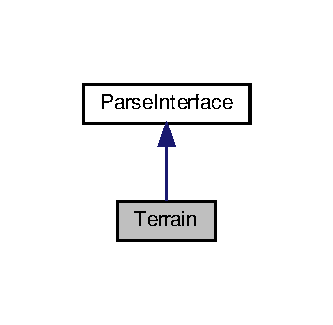
\includegraphics[width=160pt]{classTerrain__inherit__graph}
\end{center}
\end{figure}


Collaboration diagram for Terrain\+:
\nopagebreak
\begin{figure}[H]
\begin{center}
\leavevmode
\includegraphics[width=174pt]{classTerrain__coll__graph}
\end{center}
\end{figure}
\subsection*{Public Member Functions}
\begin{DoxyCompactItemize}
\item 
virtual void \hyperlink{classTerrain_a4258f6f5195a3be6c7afa3e4f03bd227}{parse\+Values} ()
\end{DoxyCompactItemize}
\subsection*{Public Attributes}
\begin{DoxyCompactItemize}
\item 
\mbox{\Hypertarget{classTerrain_a3b009bdeb1860fd2a88ed060cf0ac32b}\label{classTerrain_a3b009bdeb1860fd2a88ed060cf0ac32b}} 
std\+::vector$<$ \hyperlink{classTriangle}{Triangle} $\ast$ $>$ {\bfseries tris}
\end{DoxyCompactItemize}
\subsection*{Additional Inherited Members}


\subsection{Member Function Documentation}
\mbox{\Hypertarget{classTerrain_a4258f6f5195a3be6c7afa3e4f03bd227}\label{classTerrain_a4258f6f5195a3be6c7afa3e4f03bd227}} 
\index{Terrain@{Terrain}!parse\+Values@{parse\+Values}}
\index{parse\+Values@{parse\+Values}!Terrain@{Terrain}}
\subsubsection{\texorpdfstring{parse\+Values()}{parseValues()}}
{\footnotesize\ttfamily virtual void Terrain\+::parse\+Values (\begin{DoxyParamCaption}{ }\end{DoxyParamCaption})\hspace{0.3cm}{\ttfamily [inline]}, {\ttfamily [virtual]}}

Virtual function This is where we select what values we want to parse out of the xml file by calling the parseX functions above. 

Implements \hyperlink{classParseInterface_afca32108192ba0997c9e5a78189b0cbc}{Parse\+Interface}.



The documentation for this class was generated from the following file\+:\begin{DoxyCompactItemize}
\item 
/home/behnam/\+C\+U\+D\+A-\/\+U\+R\+B/src/Terrain.\+h\end{DoxyCompactItemize}

\hypertarget{classtest__DTEHeightField}{}\section{test\+\_\+\+D\+T\+E\+Height\+Field Class Reference}
\label{classtest__DTEHeightField}\index{test\+\_\+\+D\+T\+E\+Height\+Field@{test\+\_\+\+D\+T\+E\+Height\+Field}}
\subsection*{Public Member Functions}
\begin{DoxyCompactItemize}
\item 
\mbox{\Hypertarget{classtest__DTEHeightField_a833fda69bccf37e1e72e8d0d4cd21a89}\label{classtest__DTEHeightField_a833fda69bccf37e1e72e8d0d4cd21a89}} 
std\+::string {\bfseries main\+Test} ()
\item 
\mbox{\Hypertarget{classtest__DTEHeightField_a2a200d1cb0f75d748074b4c753b7ff3a}\label{classtest__DTEHeightField_a2a200d1cb0f75d748074b4c753b7ff3a}} 
std\+::string {\bfseries test\+Cut\+Cells} ()
\end{DoxyCompactItemize}


The documentation for this class was generated from the following files\+:\begin{DoxyCompactItemize}
\item 
/home/behnam/\+C\+U\+D\+A-\/\+U\+R\+B/src/unit\+Tests/test\+\_\+\+D\+T\+E\+Height\+Field.\+h\item 
/home/behnam/\+C\+U\+D\+A-\/\+U\+R\+B/src/unit\+Tests/test\+\_\+\+D\+T\+E\+Height\+Field.\+cpp\end{DoxyCompactItemize}

\hypertarget{classTriangle}{}\section{Triangle Class Reference}
\label{classTriangle}\index{Triangle@{Triangle}}


Inheritance diagram for Triangle\+:
\nopagebreak
\begin{figure}[H]
\begin{center}
\leavevmode
\includegraphics[width=160pt]{classTriangle__inherit__graph}
\end{center}
\end{figure}


Collaboration diagram for Triangle\+:
\nopagebreak
\begin{figure}[H]
\begin{center}
\leavevmode
\includegraphics[width=216pt]{classTriangle__coll__graph}
\end{center}
\end{figure}
\subsection*{Public Member Functions}
\begin{DoxyCompactItemize}
\item 
\mbox{\Hypertarget{classTriangle_afe6d79db021d85e6c800bc257132a9cb}\label{classTriangle_afe6d79db021d85e6c800bc257132a9cb}} 
{\bfseries Triangle} (\hyperlink{classVector3}{Vector3}$<$ float $>$ aN, \hyperlink{classVector3}{Vector3}$<$ float $>$ bN, \hyperlink{classVector3}{Vector3}$<$ float $>$ cN)
\item 
\mbox{\Hypertarget{classTriangle_a6d1204422918a61ef68fbf93cdb7fd31}\label{classTriangle_a6d1204422918a61ef68fbf93cdb7fd31}} 
float {\bfseries get\+Height\+To} (float x, float y)
\item 
\mbox{\Hypertarget{classTriangle_aaa409363ad45dbdd0348330224e971fd}\label{classTriangle_aaa409363ad45dbdd0348330224e971fd}} 
void {\bfseries get\+Boundaries} (float \&xmin, float \&xmax, float \&ymin, float \&ymax, float \&zmin, float \&zmax)
\item 
virtual void \hyperlink{classTriangle_a3b08ac99b202202bf7dbf2504da91ba1}{parse\+Values} ()
\end{DoxyCompactItemize}
\subsection*{Public Attributes}
\begin{DoxyCompactItemize}
\item 
\mbox{\Hypertarget{classTriangle_af7e91a067d28a51126e5263a5473971c}\label{classTriangle_af7e91a067d28a51126e5263a5473971c}} 
\hyperlink{classVector3}{Vector3}$<$ float $>$ $\ast$ {\bfseries a}
\item 
\mbox{\Hypertarget{classTriangle_a2bd3d9b2b01c58e95009dbbffedd2ac3}\label{classTriangle_a2bd3d9b2b01c58e95009dbbffedd2ac3}} 
\hyperlink{classVector3}{Vector3}$<$ float $>$ $\ast$ {\bfseries b}
\item 
\mbox{\Hypertarget{classTriangle_a9a9b205e19002c2142e706595913d1f5}\label{classTriangle_a9a9b205e19002c2142e706595913d1f5}} 
\hyperlink{classVector3}{Vector3}$<$ float $>$ $\ast$ {\bfseries c}
\end{DoxyCompactItemize}
\subsection*{Additional Inherited Members}


\subsection{Member Function Documentation}
\mbox{\Hypertarget{classTriangle_a3b08ac99b202202bf7dbf2504da91ba1}\label{classTriangle_a3b08ac99b202202bf7dbf2504da91ba1}} 
\index{Triangle@{Triangle}!parse\+Values@{parse\+Values}}
\index{parse\+Values@{parse\+Values}!Triangle@{Triangle}}
\subsubsection{\texorpdfstring{parse\+Values()}{parseValues()}}
{\footnotesize\ttfamily void Triangle\+::parse\+Values (\begin{DoxyParamCaption}{ }\end{DoxyParamCaption})\hspace{0.3cm}{\ttfamily [virtual]}}

Virtual function This is where we select what values we want to parse out of the xml file by calling the parseX functions above. 

Implements \hyperlink{classParseInterface_afca32108192ba0997c9e5a78189b0cbc}{Parse\+Interface}.



The documentation for this class was generated from the following files\+:\begin{DoxyCompactItemize}
\item 
/home/behnam/\+C\+U\+D\+A-\/\+U\+R\+B/src/Triangle.\+h\item 
/home/behnam/\+C\+U\+D\+A-\/\+U\+R\+B/src/Triangle.\+cpp\end{DoxyCompactItemize}

\hypertarget{classURBArgs}{}\section{U\+R\+B\+Args Class Reference}
\label{classURBArgs}\index{U\+R\+B\+Args@{U\+R\+B\+Args}}


Inheritance diagram for U\+R\+B\+Args\+:
\nopagebreak
\begin{figure}[H]
\begin{center}
\leavevmode
\includegraphics[width=172pt]{classURBArgs__inherit__graph}
\end{center}
\end{figure}


Collaboration diagram for U\+R\+B\+Args\+:
\nopagebreak
\begin{figure}[H]
\begin{center}
\leavevmode
\includegraphics[width=251pt]{classURBArgs__coll__graph}
\end{center}
\end{figure}
\subsection*{Public Member Functions}
\begin{DoxyCompactItemize}
\item 
\mbox{\Hypertarget{classURBArgs_a28039b5ab7401450959678c0a3689906}\label{classURBArgs_a28039b5ab7401450959678c0a3689906}} 
void {\bfseries process\+Arguments} (int argc, char $\ast$argv\mbox{[}$\,$\mbox{]})
\end{DoxyCompactItemize}
\subsection*{Public Attributes}
\begin{DoxyCompactItemize}
\item 
\mbox{\Hypertarget{classURBArgs_a7cec6e6267db1c1b5e923e0840f8bf9a}\label{classURBArgs_a7cec6e6267db1c1b5e923e0840f8bf9a}} 
bool {\bfseries verbose}
\item 
\mbox{\Hypertarget{classURBArgs_a2177c089cfb7963f56b14a763f288160}\label{classURBArgs_a2177c089cfb7963f56b14a763f288160}} 
std\+::string {\bfseries quic\+File} = \char`\"{}\char`\"{}
\item 
\mbox{\Hypertarget{classURBArgs_a7e9de53f20f697bf70524f6a7919ab77}\label{classURBArgs_a7e9de53f20f697bf70524f6a7919ab77}} 
std\+::string {\bfseries net\+C\+D\+F\+File} = \char`\"{}\char`\"{}
\item 
\mbox{\Hypertarget{classURBArgs_ab0f1e79a05e844622fd958420f4ed695}\label{classURBArgs_ab0f1e79a05e844622fd958420f4ed695}} 
std\+::string {\bfseries dem\+File} = \char`\"{}\char`\"{}
\item 
\mbox{\Hypertarget{classURBArgs_aa0fa7ab88f36fabed3d10b00a0cd66c9}\label{classURBArgs_aa0fa7ab88f36fabed3d10b00a0cd66c9}} 
bool {\bfseries cell\+Face}
\item 
\mbox{\Hypertarget{classURBArgs_a99598c002614de789d1e4ba21c5503ce}\label{classURBArgs_a99598c002614de789d1e4ba21c5503ce}} 
bool {\bfseries i\+Cell\+Out}
\item 
\mbox{\Hypertarget{classURBArgs_a51621034c772ef079865052bc7f8031f}\label{classURBArgs_a51621034c772ef079865052bc7f8031f}} 
bool {\bfseries terrain\+Out}
\item 
\mbox{\Hypertarget{classURBArgs_afeabfb9e13f5eb219cf2ef4d0e1b091a}\label{classURBArgs_afeabfb9e13f5eb219cf2ef4d0e1b091a}} 
bool {\bfseries solve\+Wind}
\item 
\mbox{\Hypertarget{classURBArgs_a2e78abe9008d2d774b577b95c7b99354}\label{classURBArgs_a2e78abe9008d2d774b577b95c7b99354}} 
int {\bfseries solve\+Type}
\end{DoxyCompactItemize}
\subsection*{Additional Inherited Members}


The documentation for this class was generated from the following files\+:\begin{DoxyCompactItemize}
\item 
/home/behnam/\+C\+U\+D\+A-\/\+U\+R\+B/src/handle\+U\+R\+B\+Args.\+h\item 
/home/behnam/\+C\+U\+D\+A-\/\+U\+R\+B/src/handle\+U\+R\+B\+Args.\+cpp\end{DoxyCompactItemize}

\hypertarget{classURBInputData}{}\section{U\+R\+B\+Input\+Data Class Reference}
\label{classURBInputData}\index{U\+R\+B\+Input\+Data@{U\+R\+B\+Input\+Data}}


Inheritance diagram for U\+R\+B\+Input\+Data\+:
\nopagebreak
\begin{figure}[H]
\begin{center}
\leavevmode
\includegraphics[width=161pt]{classURBInputData__inherit__graph}
\end{center}
\end{figure}


Collaboration diagram for U\+R\+B\+Input\+Data\+:
\nopagebreak
\begin{figure}[H]
\begin{center}
\leavevmode
\includegraphics[width=350pt]{classURBInputData__coll__graph}
\end{center}
\end{figure}
\subsection*{Public Member Functions}
\begin{DoxyCompactItemize}
\item 
virtual void \hyperlink{classURBInputData_a3fea38ec8d574eb8e5c9ee5f1ad53636}{parse\+Values} ()
\end{DoxyCompactItemize}
\subsection*{Public Attributes}
\begin{DoxyCompactItemize}
\item 
\mbox{\Hypertarget{classURBInputData_acf42beaabf93d0d6fd3b0837848bf159}\label{classURBInputData_acf42beaabf93d0d6fd3b0837848bf159}} 
\hyperlink{classSimulationParameters}{Simulation\+Parameters} $\ast$ {\bfseries sim\+Params}
\item 
\mbox{\Hypertarget{classURBInputData_a33d069c2768f3aa4611418882b89cae2}\label{classURBInputData_a33d069c2768f3aa4611418882b89cae2}} 
\hyperlink{classFileOptions}{File\+Options} $\ast$ {\bfseries file\+Options}
\item 
\mbox{\Hypertarget{classURBInputData_a25b7c100a2265dd5d2bb8212a35d4e5b}\label{classURBInputData_a25b7c100a2265dd5d2bb8212a35d4e5b}} 
\hyperlink{classMetParams}{Met\+Params} $\ast$ {\bfseries met\+Params}
\item 
\mbox{\Hypertarget{classURBInputData_abe9776ac2268dc4783e29e90e9c70ff3}\label{classURBInputData_abe9776ac2268dc4783e29e90e9c70ff3}} 
\hyperlink{classBuildings}{Buildings} $\ast$ {\bfseries buildings}
\end{DoxyCompactItemize}
\subsection*{Additional Inherited Members}


\subsection{Member Function Documentation}
\mbox{\Hypertarget{classURBInputData_a3fea38ec8d574eb8e5c9ee5f1ad53636}\label{classURBInputData_a3fea38ec8d574eb8e5c9ee5f1ad53636}} 
\index{U\+R\+B\+Input\+Data@{U\+R\+B\+Input\+Data}!parse\+Values@{parse\+Values}}
\index{parse\+Values@{parse\+Values}!U\+R\+B\+Input\+Data@{U\+R\+B\+Input\+Data}}
\subsubsection{\texorpdfstring{parse\+Values()}{parseValues()}}
{\footnotesize\ttfamily void U\+R\+B\+Input\+Data\+::parse\+Values (\begin{DoxyParamCaption}{ }\end{DoxyParamCaption})\hspace{0.3cm}{\ttfamily [inline]}, {\ttfamily [virtual]}}

Virtual function This is where we select what values we want to parse out of the xml file by calling the parseX functions above. 

Implements \hyperlink{classParseInterface_afca32108192ba0997c9e5a78189b0cbc}{Parse\+Interface}.



The documentation for this class was generated from the following files\+:\begin{DoxyCompactItemize}
\item 
/home/behnam/\+C\+U\+D\+A-\/\+U\+R\+B/src/U\+R\+B\+Input\+Data.\+h\item 
/home/behnam/\+C\+U\+D\+A-\/\+U\+R\+B/src/U\+R\+B\+Input\+Data.\+cpp\end{DoxyCompactItemize}

\hypertarget{classVector3}{}\section{Vector3$<$ T $>$ Class Template Reference}
\label{classVector3}\index{Vector3$<$ T $>$@{Vector3$<$ T $>$}}


Inheritance diagram for Vector3$<$ T $>$\+:
\nopagebreak
\begin{figure}[H]
\begin{center}
\leavevmode
\includegraphics[width=160pt]{classVector3__inherit__graph}
\end{center}
\end{figure}


Collaboration diagram for Vector3$<$ T $>$\+:
\nopagebreak
\begin{figure}[H]
\begin{center}
\leavevmode
\includegraphics[width=174pt]{classVector3__coll__graph}
\end{center}
\end{figure}
\subsection*{Public Member Functions}
\begin{DoxyCompactItemize}
\item 
\mbox{\Hypertarget{classVector3_a4f08341de72b29b98df76f81eaf6d4f0}\label{classVector3_a4f08341de72b29b98df76f81eaf6d4f0}} 
{\footnotesize template$<$typename X $>$ }\\{\bfseries Vector3} (const \hyperlink{classX}{X} a, const \hyperlink{classX}{X} b, const \hyperlink{classX}{X} c)
\item 
virtual void \hyperlink{classVector3_a15a1271a3ba4497ca95cc4dd66481f9e}{parse\+Values} ()
\item 
\mbox{\Hypertarget{classVector3_a9833b43da58a55b3d466c576be10bad5}\label{classVector3_a9833b43da58a55b3d466c576be10bad5}} 
T \& {\bfseries operator\mbox{[}$\,$\mbox{]}} (const int i)
\item 
\mbox{\Hypertarget{classVector3_a2a17ca1fc283c97c240b5fabcf1de375}\label{classVector3_a2a17ca1fc283c97c240b5fabcf1de375}} 
bool {\bfseries operator==} (\hyperlink{classVector3}{Vector3}$<$ T $>$ \&v)
\item 
virtual void \hyperlink{classVector3_a15a1271a3ba4497ca95cc4dd66481f9e}{parse\+Values} ()
\item 
\mbox{\Hypertarget{classVector3_a6fd34fef8f2a085889138fbb9e437f4d}\label{classVector3_a6fd34fef8f2a085889138fbb9e437f4d}} 
int \& {\bfseries operator\mbox{[}$\,$\mbox{]}} (const int i)
\end{DoxyCompactItemize}
\subsection*{Protected Attributes}
\begin{DoxyCompactItemize}
\item 
\mbox{\Hypertarget{classVector3_a9ca9d69851a096e97b03ee62a7fbbb99}\label{classVector3_a9ca9d69851a096e97b03ee62a7fbbb99}} 
std\+::vector$<$ T $>$ {\bfseries values}
\end{DoxyCompactItemize}
\subsection*{Additional Inherited Members}


\subsection{Member Function Documentation}
\mbox{\Hypertarget{classVector3_a15a1271a3ba4497ca95cc4dd66481f9e}\label{classVector3_a15a1271a3ba4497ca95cc4dd66481f9e}} 
\index{Vector3@{Vector3}!parse\+Values@{parse\+Values}}
\index{parse\+Values@{parse\+Values}!Vector3@{Vector3}}
\subsubsection{\texorpdfstring{parse\+Values()}{parseValues()}\hspace{0.1cm}{\footnotesize\ttfamily [1/2]}}
{\footnotesize\ttfamily template$<$class T$>$ \\
virtual void \hyperlink{classVector3}{Vector3}$<$ T $>$\+::parse\+Values (\begin{DoxyParamCaption}{ }\end{DoxyParamCaption})\hspace{0.3cm}{\ttfamily [inline]}, {\ttfamily [virtual]}}

Virtual function This is where we select what values we want to parse out of the xml file by calling the parseX functions above. 

Implements \hyperlink{classParseInterface_afca32108192ba0997c9e5a78189b0cbc}{Parse\+Interface}.

\mbox{\Hypertarget{classVector3_a15a1271a3ba4497ca95cc4dd66481f9e}\label{classVector3_a15a1271a3ba4497ca95cc4dd66481f9e}} 
\index{Vector3@{Vector3}!parse\+Values@{parse\+Values}}
\index{parse\+Values@{parse\+Values}!Vector3@{Vector3}}
\subsubsection{\texorpdfstring{parse\+Values()}{parseValues()}\hspace{0.1cm}{\footnotesize\ttfamily [2/2]}}
{\footnotesize\ttfamily template$<$class T$>$ \\
virtual void \hyperlink{classVector3}{Vector3}$<$ T $>$\+::parse\+Values (\begin{DoxyParamCaption}{ }\end{DoxyParamCaption})\hspace{0.3cm}{\ttfamily [inline]}, {\ttfamily [virtual]}}

Virtual function This is where we select what values we want to parse out of the xml file by calling the parseX functions above. 

Implements \hyperlink{classParseInterface_afca32108192ba0997c9e5a78189b0cbc}{Parse\+Interface}.



The documentation for this class was generated from the following file\+:\begin{DoxyCompactItemize}
\item 
/home/behnam/\+C\+U\+D\+A-\/\+U\+R\+B/src/Vector3.\+h\end{DoxyCompactItemize}

\hypertarget{classX}{}\section{X Class Reference}
\label{classX}\index{X@{X}}


Inheritance diagram for X\+:
\nopagebreak
\begin{figure}[H]
\begin{center}
\leavevmode
\includegraphics[width=160pt]{classX__inherit__graph}
\end{center}
\end{figure}


Collaboration diagram for X\+:
\nopagebreak
\begin{figure}[H]
\begin{center}
\leavevmode
\includegraphics[width=311pt]{classX__coll__graph}
\end{center}
\end{figure}
\subsection*{Public Member Functions}
\begin{DoxyCompactItemize}
\item 
void \hyperlink{classX_a0d0aabf7efbe8356894613e58b736216}{parse\+Values} ()
\end{DoxyCompactItemize}
\subsection*{Public Attributes}
\begin{DoxyCompactItemize}
\item 
\mbox{\Hypertarget{classX_a2370d2f6fd5440bf742ac758d329ae53}\label{classX_a2370d2f6fd5440bf742ac758d329ae53}} 
\hyperlink{classA}{A} $\ast$ {\bfseries a\+Var}
\item 
\mbox{\Hypertarget{classX_afa6720354fe2a87c02283955f9054157}\label{classX_afa6720354fe2a87c02283955f9054157}} 
\hyperlink{classB}{B} $\ast$ {\bfseries b\+Var}
\item 
\mbox{\Hypertarget{classX_a462350abfcbb7aa3411cc323ca69ff3d}\label{classX_a462350abfcbb7aa3411cc323ca69ff3d}} 
\hyperlink{classC}{C} $\ast$ {\bfseries c\+Var}
\item 
\mbox{\Hypertarget{classX_a9054178c4e8bd30504714f4464796557}\label{classX_a9054178c4e8bd30504714f4464796557}} 
\hyperlink{classD}{D} $\ast$ {\bfseries d\+Var}
\item 
\mbox{\Hypertarget{classX_aae69f92ec873d2f4325cb38bf1560608}\label{classX_aae69f92ec873d2f4325cb38bf1560608}} 
\hyperlink{classP}{P} $\ast$ {\bfseries p\+Var}
\item 
\mbox{\Hypertarget{classX_a129a83c087a5e9dc2895ebf74bd2d39d}\label{classX_a129a83c087a5e9dc2895ebf74bd2d39d}} 
int {\bfseries x}
\end{DoxyCompactItemize}
\subsection*{Additional Inherited Members}


\subsection{Member Function Documentation}
\mbox{\Hypertarget{classX_a0d0aabf7efbe8356894613e58b736216}\label{classX_a0d0aabf7efbe8356894613e58b736216}} 
\index{X@{X}!parse\+Values@{parse\+Values}}
\index{parse\+Values@{parse\+Values}!X@{X}}
\subsubsection{\texorpdfstring{parse\+Values()}{parseValues()}}
{\footnotesize\ttfamily void X\+::parse\+Values (\begin{DoxyParamCaption}{ }\end{DoxyParamCaption})\hspace{0.3cm}{\ttfamily [inline]}, {\ttfamily [virtual]}}

Virtual function This is where we select what values we want to parse out of the xml file by calling the parseX functions above. 

Implements \hyperlink{classParseInterface_afca32108192ba0997c9e5a78189b0cbc}{Parse\+Interface}.



The documentation for this class was generated from the following file\+:\begin{DoxyCompactItemize}
\item 
/home/behnam/\+C\+U\+D\+A-\/\+U\+R\+B/xml\+Testing/X.\+h\end{DoxyCompactItemize}

%--- End generated contents ---

% Index
\backmatter
\newpage
\phantomsection
\clearemptydoublepage
\addcontentsline{toc}{chapter}{Index}
\printindex

\end{document}
